%%%%%%%%%%%%%%%%%%%%%%%%%%%%%%%%%%%%%%%%%%%%%%%%%%%
%
%  New template code for TAMU Theses and Dissertations starting Spring 2018.  
%
%
%  Author: Sean Zachary Roberson
%  Version 3.17.09
%  Last Updated: 9/21/2017
%
%%%%%%%%%%%%%%%%%%%%%%%%%%%%%%%%%%%%%%%%%%%%%%%%%%%

% NOTE: THE ONLY MAJOR CHANGE IS IN THE RELAXATION
% OF MARGIN REQUIREMENTS. THIS TEMPLATE IS THE MOST
% CURRENT. SEE THE FILES README.TXT AND NEWCHANGES.TXT
% FOR MORE INFORMATION.

\documentclass[12pt]{report}

\usepackage{tamuconfig}
\usepackage{booktabs}
% Most of the packages that set the default settings
% for the document have moved to the style file
% tamuconfig.sty. This includes

%These next lines change the font. Fixes for certain
%fonts will be implemented in a future release.

%Comment this line if you do not wish to use Times
%New Roman. The font used will then be the LaTeX
%default of Computer Modern.
\usepackage{times}
%\usepackage{cmbright}
\usepackage[T1]{fontenc}

% For natbib-style references, uncomment this.
%\usepackage{natbib}

%This package allows for the use of graphics in the
%document.
\usepackage{graphicx}

%If you have JPEG format images, add .jpg as an
%allowed file extension below. Same for Bitmaps (.bmp).
\DeclareGraphicsExtensions{.png}

%It is best practice to keep all your pictures in
%one folder inside the main directory in which your
%TeX file is kept. Here the folder is named "graphic."
%Replace the name here with your folder's name, if needed.
%The period is needed due to relative referencing.
\graphicspath{ {./graphic/} }

% For quick document navigation.
\usepackage[hidelinks]{hyperref}

%%%%%%%%%%%%%%%%%%%%%%%%%%%%%%%%%%%%%%%%%%%%%%%%%%%%%%%%%
%Please place all your personal packages here. Check to
%see if the packages you wish to use are not already
%declared above. Placing all your personal packages
%here allows me to determine if there are any package
%issues in compilation, as well as any conflicts
%that may arise by the order of loading.
%--Sean Zachary Roberson
%%%%%%%%%%%%%%%%%%%%%%%%%%%%%%%%%%%%%%%%%%%%%%%%%%%%%%%%%
%%%%%%%%%%%%%%%%%%%%%%%%%%%%%%%%%%%%%%%%%%%%%%%%%%%%%%%%%
%Begin student defined packages.
%%%%%%%%%%%%%%%%%%%%%%%%%%%%%%%%%%%%%%%%%%%%%%%%%%%%%%%%%


%%%%%%%%%%%%%%%%%%%%%%%%%%%%%%%%%%%%%%%%%%%%%%%%%%%%%%%%%
%End student defined packages.
%%%%%%%%%%%%%%%%%%%%%%%%%%%%%%%%%%%%%%%%%%%%%%%%%%%%%%%%%

% End preamble. Document begins below.

\begin{document}

%The title of your document goes here.
%Spacing may need to be adjusted if your title is long
%and pushes the copyright off the page.
\renewcommand{\tamumanuscripttitle}{Radio Altimeter Tolerance of Wireless Avionics Intra-Communications Systems}

%Type only Thesis, Dissertation, or Record of Study.
\renewcommand{\tamupapertype}{Thesis}

%Your full name goes here, as it is in university records. Check your student record on Howdy if there is any mismatch.
\renewcommand{\tamufullname}{Joshua Thomas Ruff}

%The degree title goes here. See the OGAPS site for more info.
\renewcommand{\tamudegree}{Master of Science}
\renewcommand{\tamuchairone}{Gregory H. Huff}


% Uncomment out the next line if you have co-chairs.  You will also need to edit the titlepage.tex file.
\newcommand{\tamuchairtwo}{Jean-Francois Chamberland}
\renewcommand{\tamumemberone}{Robert D. Nevels}
\newcommand{\tamumembertwo}{Darren Hartl}
%\newcommand{\tamumemberthree}{Committee Member 3}
\renewcommand{\tamudepthead}{Miroslav M. Begovic}

%Type only May, August, or December.
\renewcommand{\tamugradmonth}{May}
\renewcommand{\tamugradyear}{2019}
%Your department name goes here.
\renewcommand{\tamudepartment}{Electrical Engineering}


%%%%%%%%%%%%%%%%%%%%%%%%%%%%%%%%%%%%%%%%%%%%%%%%%%%
%
%  New template code for TAMU Theses and Dissertations starting Fall 2016.  
%
%
%  Author: Sean Zachary Roberson
%  Version 3.17.09
%  Last Updated: 9/21/2017
%
%%%%%%%%%%%%%%%%%%%%%%%%%%%%%%%%%%%%%%%%%%%%%%%%%%%

%%%%%%%%%%%%%%%%%%%%%%%%%%%%%% 
%% TITLE PAGE
%% The values get updated automatically.  Please do not make changes to this file other than adding/deleting committee members where necessary.
%%%%%%%%%%%%%%%%%%%%%%%%%%%%%%

\providecommand{\tabularnewline}{\\}



\begin{titlepage}
\begin{center}
\MakeUppercase{\tamumanuscripttitle}
\vspace{4em}

A \tamupapertype

by

\MakeUppercase{\tamufullname}

\vspace{4em}

\begin{singlespace}

Submitted to the Office of Graduate and Professional Studies of \\
Texas A\&M University \\

in partial fulfillment of the requirements for the degree of \\
\end{singlespace}

\MakeUppercase{\tamudegree}
\par\end{center}
\vspace{2em}
\begin{singlespace}
\begin{tabular}{ll}
 & \tabularnewline
& \cr
% If you have Co-Chairs comment out the 'Chair of Committee' line below and uncomment the 'Co-Chairs of Committee' line.
Chair of Committee, & \tamuchairone\tabularnewline
%Co-Chairs of Committee, & \tamuchairone\tabularnewline & \tamuchairtwo\tabularnewline
Committee Members, & \tamumemberone\tabularnewline
 & \tamumembertwo\tabularnewline
 & \tamumemberthree\tabularnewline
Head of Department, & \tamudepthead\tabularnewline

\end{tabular}
\end{singlespace}
\vspace{3em}

\begin{center}
\tamugradmonth \hspace{2pt} \tamugradyear

\vspace{3em}

Major Subject: \tamudepartment \par
\vspace{3em}
Copyright \tamugradyear \hspace{.5em}\tamufullname 
\par\end{center}
\end{titlepage}
\pagebreak{}




 % This is simply a file that formats and adds your titlepage, please do not edit this unless you have a specific need. .
%%%%%%%%%%%%%%%%%%%%%%%%%%%%%%%%%%%%%%%%%%%%%%%%%%%
%
%  New template code for TAMU Theses and Dissertations starting Fall 2016.  
%
%
%  Author: Sean Zachary Roberson
%  Version 3.17.09
%  Last Updated: 9/21/2017
%
%%%%%%%%%%%%%%%%%%%%%%%%%%%%%%%%%%%%%%%%%%%%%%%%%%%
%%%%%%%%%%%%%%%%%%%%%%%%%%%%%%%%%%%%%%%%%%%%%%%%%%%%%%%%%%%%%%%%%%%%%
%%                           ABSTRACT 
%%%%%%%%%%%%%%%%%%%%%%%%%%%%%%%%%%%%%%%%%%%%%%%%%%%%%%%%%%%%%%%%%%%%%

\chapter*{ABSTRACT}
\addcontentsline{toc}{chapter}{ABSTRACT} % Needs to be set to part, so the TOC doesnt add 'CHAPTER ' prefix in the TOC.

\pagestyle{plain} % No headers, just page numbers
\pagenumbering{roman} % Roman numerals
\setcounter{page}{2}

\indent This is the first numbered page, lower case Roman numberal (ii). Page numbers are outside the prescribed margins, at the bottom of the page and centered; everything else is inside the margins.No bold on this page (Exception: heading ABSTRACT is bold if major headings are bold. \emph{This \LaTeX ~ template applies to this exception}).

Text begins two double spaces below the major heading. Recommended length of text is no more than 350 words. Vertical spacing is double spaced or space-and-a-half. (\emph{This \LaTeX ~ template applies double space for this ABSTRACT.}) The same margin settings and text alignment are followed else where in this thesis. There should be no numbered references or formal citations in ABSTRACT.

The content of this ABSTRACT provides a complete, succinct snapshot of the research, addressing the purpose, methods, results, and conclusions of the research. As a result, it should stand alone without any formal citations or references to chapters/sections of the work. To accomodate with a variety of online database, images or complex equations should also be avoided.

The next pages are Dedication, Acknowledgments, Contributors and Funding Sources, and Nomenclature. Of these, Contributors and Funding Sources is required. The rest are optional.


 

\pagebreak{}

%%%%%%%%%%%%%%%%%%%%%%%%%%%%%%%%%%%%%%%%%%%%%%%%%%%%
%
%  New template code for TAMU Theses and Dissertations starting Fall 2016.  
%
%
%  Author: Sean Zachary Roberson
%  Version 3.17.09
%  Last Updated: 9/21/2017
%
%%%%%%%%%%%%%%%%%%%%%%%%%%%%%%%%%%%%%%%%%%%%%%%%%%%

%%%%%%%%%%%%%%%%%%%%%%%%%%%%%%%%%%%%%%%%%%%%%%%%%%%%%%%%%%%%%%%%%%%%%%
%%                           DEDICATION
%%%%%%%%%%%%%%%%%%%%%%%%%%%%%%%%%%%%%%%%%%%%%%%%%%%%%%%%%%%%%%%%%%%%%
\chapter*{DEDICATION}
\addcontentsline{toc}{chapter}{DEDICATION}  % Needs to be set to part, so the TOC doesnt add 'CHAPTER ' prefix in the TOC.



\begin{center}
\vspace*{\fill}
To my mother, my father, my grandfather, and my grandmother. To see what happens with multiple lines, I extend this next part into a second line.
\vspace*{\fill}
\end{center}

\pagebreak{}

%%%%%%%%%%%%%%%%%%%%%%%%%%%%%%%%%%%%%%%%%%%%%%%%%%%
%
%  New template code for TAMU Theses and Dissertations starting Fall 2016.  
%
%
%  Author: Sean Zachary Roberson
%  Version 3.17.09
%  Last Updated: 9/21/2017
%
%%%%%%%%%%%%%%%%%%%%%%%%%%%%%%%%%%%%%%%%%%%%%%%%%%%


%%%%%%%%%%%%%%%%%%%%%%%%%%%%%%%%%%%%%%%%%%%%%%%%%%%%%%%%%%%%%%%%%%%%%%
%%                           ACKNOWLEDGMENTS
%%%%%%%%%%%%%%%%%%%%%%%%%%%%%%%%%%%%%%%%%%%%%%%%%%%%%%%%%%%%%%%%%%%%%
\chapter*{ACKNOWLEDGMENTS}
\addcontentsline{toc}{chapter}{ACKNOWLEDGMENTS}  % Needs to be set to part, so the TOC doesnt add 'CHAPTER ' prefix in the TOC.


\indent I would like to thank my advisor, Dr. Huff, for giving me the opportunity to work in his lab throughout undergraduate and graduate school. Under his mentorship, my interest in electromagnetics developed into a passion which has driven my career. I would also like to thank Dr. Chamberland, who provided advice and professional guidance as I navigated undergraduate research and graduate school. Additionally, I would like to thank Dr. Fred Fisher and Dr. Dave Redman for their support over the years, especially through the transition period which followed Dr. Huff's move. Without them I could not have graduated when I did. Finally, I would like to thank my parents for their constant love and support while I attended graduate school. 

\pagebreak{}
%%%%%%%%%%%%%%%%%%%%%%%%%%%%%%%%%%%%%%%%%%%%%%%%%%%
%
%  New template code for TAMU Theses and Dissertations starting Fall 2016.  
%
%
%  Author: Sean Zachary Roberson
%  Version 3.17.09
%  Last Updated: 9/21/2017
%
%%%%%%%%%%%%%%%%%%%%%%%%%%%%%%%%%%%%%%%%%%%%%%%%%%%


%%%%%%%%%%%%%%%%%%%%%%%%%%%%%%%%%%%%%%%%%%%%%%%%%%%%%%%%%%%%%%%%%%%%%%
%%             CONTRIBUTORS AND FUNDING SOURCES
%%%%%%%%%%%%%%%%%%%%%%%%%%%%%%%%%%%%%%%%%%%%%%%%%%%%%%%%%%%%%%%%%%%%%
\chapter*{CONTRIBUTORS AND FUNDING SOURCES}
\addcontentsline{toc}{chapter}{CONTRIBUTORS AND FUNDING SOURCES}  % Needs to be set to part, so the TOC doesn't add 'CHAPTER ' prefix in the TOC.

This work was sponsored by the Aerospace Vehicles Systems Institute (AVSI) through Authorization for Expenditure 76s1 (AFE 76s1). Project members contributed funding, equipment, and expertise without which the project would not have been completed. Project members included Honeywell*, Rockwell Collins*, Thales*, Garmin*, Airbus, Boeing, Embraer, Lufthansa, UTC, Zodiac, NASA, FAA, IATA. Starred project members contributed widely used commercial radio altimeters for testing.  

Thomas Meyerhoff from Airbus contributed the worst case landing scenario analysis covered in Section~\ref{subsub:worst_case}, and the summary of initial testing results shown in Figure~\ref{fig:initial_summary}. Dr. Chadi Geha provided the concept for the modified altimeter test setup shown in Figure~\ref{fig:Modified}. All other work presented in this thesis was conducted by the author. 

\pagebreak{}
%%%%%%%%%%%%%%%%%%%%%%%%%%%%%%%%%%%%%%%%%%%%%%%%%%%%
%
%  New template code for TAMU Theses and Dissertations starting Fall 2016.  
%
%
%  Author: Sean Zachary Roberson
%  Version 3.17.09
%  Last Updated: 9/21/2017
%
%%%%%%%%%%%%%%%%%%%%%%%%%%%%%%%%%%%%%%%%%%%%%%%%%%%

%%%%%%%%%%%%%%%%%%%%%%%%%%%%%%%%%%%%%%%%%%%%%%%%%%%%%%%%%%%%%%%%%%%%%%
%%                           NOMENCLATURE
%%%%%%%%%%%%%%%%%%%%%%%%%%%%%%%%%%%%%%%%%%%%%%%%%%%%%%%%%%%%%%%%%%%%%

\chapter*{NOMENCLATURE}
\addcontentsline{toc}{chapter}{NOMENCLATURE}  % Needs to be set to part, so the TOC doesnt add 'CHAPTER ' prefix in the TOC.

%A note about aligning: These entries will align
%themselves according to the ampersand (&).
%No extra spaces are needed, as seen in some of
%the entries below.

%Example of the longtable environment.
\hspace*{-1.25in}
\vspace{12pt}
\begin{spacing}{1.0}
	\begin{longtable}[htbp]{@{}p{0.35\textwidth} p{0.62\textwidth}@{}}
	   % \begin{tabular}{@{}p{0.33\textwidth} p{0.62\textwidth}@{}}
		OGAPS	&	Office of Graduate and Professional Studies at Texas A\&M University\\	[2ex]
		B/CS		&	Bryan and College Station\\	[2ex] %[2ex] provides double space between each row
		TAMU			&	Texas A\&M University\\	[2ex]
		SDCC & San Diego Comic-Con\\ [2ex]
		EVIL & Every Villain is Lemons\\ [2ex]
		EPCC & Educator Preparation and Certification Center at Texas A\&M University - San Antonio\\ [2ex]
		FFT & Fast Fourier Transform\\ [2ex]
		ARIMA & Autoregressive Integrated Moving Average\\ [2ex]
		SSD & Solid State Drive\\ [2ex]
		HDD & Hard Disk Drive\\ [2ex]
		O\&M & Eller Oceanography and Meteorology Building\\ [2ex]
		DOS & Disk Operating System\\ [2ex]
		HDMI & High Definition Multimedia Interface\\ [2ex]
		$L^1$ & Space of absolutely Lebesgue integrable functions; i.e., $\int |f| < \infty$\\ [2ex]
		$L^2$ & Space of square-Lebesgue-integrable functions, i.e., $\int |f|^2 < \infty$\\ [2ex]
		$PC(S)$ & Space of piecewise-continuous functions on $S$\\ [2ex]
		GNU & GNU is Not Unix\\ [2ex]
		GUI & Graphical User Interface\\ [2ex]
		PID & Principal Integral Domain\\ [2ex]
		MIP & Mixed Integer Program\\ [2ex]
		LP & Linear Program\\ [2ex]
		%XXXXXXXX		&	This is an optional page. Random word to test how long the sentence can be? This is just for test purpose. The current setting aims to align left/right margin same as all other pages.\\	[2ex]
	   % \end{tabular}%
	\end{longtable}
\end{spacing}

\pagebreak{}

%%%%%%%%%%%%%%%%%%%%%%%%%%%%%%%%%%%%%%%%%%%%%%%%%%%
%
%  New template code for TAMU Theses and Dissertations starting Fall 2016.  
%
%
%  Author: Sean Zachary Roberson
%  Version 3.17.09
%  Last Updated: 9/21/2017
%
%%%%%%%%%%%%%%%%%%%%%%%%%%%%%%%%%%%%%%%%%%%%%%%%%%%
%%%%%%%%%%%%%%%%%%%%%%%%%%%%%%%%%%%%%%%%%%%%%%%%%%%%%%%%%%%%%%%%%%%%%%
%%       TABLE OF CONTENTS
%%%%%%%%%%%%%%%%%%%%%%%%%%%%%%%%%%%%%%%%%%%%%%%%%%%%%%%%%%%%%%%%%%%%%
% single-space sections in Table of Contents  - commented in version 1.7
%\renewcommand{\cftsecafterpnum}{\vskip0.5\baselineskip}
%\renewcommand{\cftsubsecafterpnum}{\vskip0.5\baselineskip}
%\renewcommand{\cftsubsubsecafterpnum}{\vskip0.5\baselineskip}
%%%%%%%%%%%%%%%%%%%%%%%%%%%%%%%%%%%%%%%%%%%%%%%%%%%

\phantomsection
\addcontentsline{toc}{chapter}{TABLE OF CONTENTS}  

\begin{singlespace}
\renewcommand\contentsname{\normalfont} {\centerline{TABLE OF CONTENTS}}

\setcounter{tocdepth}{4} % This puts \subsubsection[]{×} in your List of Tables.  The default is 3.


%%%%%%%%%%%%%  Adds Page above the page number in TOC
\setlength{\cftaftertoctitleskip}{1em}
\renewcommand{\cftaftertoctitle}{%
\hfill{\normalfont {Page}\par}}


\tableofcontents

%\addtocontents{toc}{\protect\afterpage{~\hfill\normalfont{Page}\par\medskip}}
\end{singlespace}

\pagebreak{}

%%%%%%%%%%%%%%%%%%%%%%%%%%%%%%%%%%%%%%%%%%%%%%%%%%%%%%%%%%%%%%%%%%%%%%
%%                           LIST OF FIGURES
%%%%%%%%%%%%%%%%%%%%%%%%%%%%%%%%%%%%%%%%%%%%%%%%%%%%%%%%%%%%%%%%%%%%%

\phantomsection
\addcontentsline{toc}{chapter}{LIST OF FIGURES}  

\renewcommand{\cftloftitlefont}{\center\normalfont\MakeUppercase}

\setlength{\cftbeforeloftitleskip}{-12pt} %% Positions the LOF title vertically to match the chapter titles
\renewcommand{\cftafterloftitleskip}{12pt}


\renewcommand{\cftafterloftitle}{%
\\[4em]\mbox{}\hspace{2pt}FIGURE\hfill{\normalfont Page}\vskip\baselineskip}

\begingroup


\begin{center}
\begin{singlespace}
%% These values make the lof table entries appear double spaced between.
\setlength{\cftbeforechapskip}{0.4cm}
\setlength{\cftbeforesecskip}{0.30cm}
\setlength{\cftbeforesubsecskip}{0.30cm}
\setlength{\cftbeforefigskip}{0.4cm}
\setlength{\cftbeforetabskip}{0.4cm}

% Provided by Andy Philips.
% needed to make chapter gaps look no different than sections:
% \addtocontents{lof}{\protect\renewcommand*\protect\addvspace[1]{}}

% Philips' document had 30 figures. Is there a maximum number of figures
% that changes the spacing to non-uniform, i.e., not double-spaced
% between all entries?

\listoffigures

\end{singlespace}
\end{center}

\pagebreak{}


%%%%%%%%%%%%%%%%%%%%%%%%%%%%%%%%%%%%%%%%%%%%%%%%%%%%%%%%%%%%%%%%%%%%%%
%%                           LIST OF TABLES
%%%%%%%%%%%%%%%%%%%%%%%%%%%%%%%%%%%%%%%%%%%%%%%%%%%%%%%%%%%%%%%%%%%%%%
%
\phantomsection
\addcontentsline{toc}{chapter}{LIST OF TABLES}  

\renewcommand{\cftlottitlefont}{\center\normalfont\MakeUppercase}

\setlength{\cftbeforelottitleskip}{-12pt} %% Positions the LOT title vertically to match the chapter titles

%Note that the similar parameter in the LOF is 12pt; this
%is intentional to make the spacing between the headers
%and the first entry look consistent.
\renewcommand{\cftafterlottitleskip}{1pt}


\renewcommand{\cftafterlottitle}{%
\\[4em]\mbox{}\hspace{2pt}TABLE\hfill{\normalfont Page}\vskip\baselineskip}

\begin{center}
\begin{singlespace}

%% These values make the lot table entries appear double spaced between.
\setlength{\cftbeforechapskip}{0.4cm}
\setlength{\cftbeforesecskip}{0.30cm}
\setlength{\cftbeforesubsecskip}{0.30cm}
\setlength{\cftbeforefigskip}{0.4cm}
\setlength{\cftbeforetabskip}{0.4cm}

\listoftables 

\end{singlespace}
\end{center}
\endgroup
\pagebreak{}  % Need this for the pagenumbering to be correct.   % This is simply a file that formats and adds your toc, lof, and lot, please do not edit this unless you have a specific need.

%%%%%%%%%%%%%%%%%%%%%%%%%%%%%%%%%%%%%%%%%%%%%%%%%%%
%
%  New template code for TAMU Theses and Dissertations starting Fall 2016.  
%
%
%  Author: Sean Zachary Roberson
%  Version 3.17.09
%  Last Updated: 9/21/2017
%
%%%%%%%%%%%%%%%%%%%%%%%%%%%%%%%%%%%%%%%%%%%%%%%%%%%

%%%%%%%%%%%%%%%%%%%%%%%%%%%%%%%%%%%%%%%%%%%%%%%%%%%%%%%%%%%%%%%%%%%%%%
%%                           SECTION I
%%%%%%%%%%%%%%%%%%%%%%%%%%%%%%%%%%%%%%%%%%%%%%%%%%%%%%%%%%%%%%%%%%%%%


\pagestyle{plain} % No headers, just page numbers
\pagenumbering{arabic} % Arabic numerals
\setcounter{page}{1}


\chapter{\uppercase {Introduction}}


\section{Motivation}

Over the past two decades, wireless digital communication systems have become ubiquitous in the public life. As the technologies have become more proven, a broad range of players in the aerospace industry developed a significant interest in deploying these systems to electronics on airplanes. Specifically, these companies are interested in radiocommunication between devices on a single aircraft related to the regularity and safety of flight, rather than communications outside an aircraft or for passenger entertainment~\cite{redman_waic_2011}. 

Avionics manufacturers are interested in the development, sale and deployment of sensors and devices in areas on a plane that were difficult or impossible to reach with wireless systems.  Examples might include placing sensors to monitor a landing gear or internal to an engine, where rotating parts make monitoring difficult~\cite{redman_waic_2011}. Airframers, Aircraft OEMs and Airlines all have a vested interest in any development which could reduce the amount of copper wiring on planes, thus reducing weight and fuel costs~\cite{canaday_war_2017}. Regulators are interested in wireless avionics systems from a safety perspective. Critical avionics systems have redundant paths wired in in case of failure, and some or all of these redundancies may eventually be replaced  with wireless ones~\cite{canaday_war_2017}~\cite{redman_waic_2011}. This type of dissimilar redundancy is always appealing from a safety perspective. The classic example of an engine fire which destroys the physical connection to a controller (and so can't be shut off) demonstrates the utility of a wireless backup~\cite{redman_waic_2011}.

\section{History} 

With these diverse motivations spanning across the industry, various aerospace companies sponsored a series of working groups to implement wireless communications systems on aircraft. This systems used in this class of applications were alternatively called Wireless Sensing Networks (WSN's) in early literature, and Wireless Avionics Intra-Communications (WAIC) systems later on. WAIC related projects were sponsored and conducted through the Aerospace Vehicle Systems Institute (AVSI), which also directed this project. AVSI projects are funded through independent grants known as Authorizations For Expenditure (AFEs)

Three AVSI projects directly relate to WAIC: AFE 56, AFE 73, and AFE 76. AFE 56 studied the feasibility of potential WAIC systems  and investigated the suitability of various bands to WAIC applications. AFE 73 took the analysis done by AFE 56 and used the work to advocate to regulators for spectrum allocation for WAIC. 

\section{Project Goals}
This work was funded through AVSI and managed under AFE 76. Project members include but are not limited to Airbus, Boeing, Honeywell, NASA, Rockwell Collins, Thales, and Garmin. All members contributed funding, technical, and material support to this project. The goal of this project are to perform a band sharing study for WAIC with radio altimeters, to develop a prototype for WAIC systems, and develop the regulatory documentation necessary for the certification of WAIC systems. 

The technical challenges in this project directly result from both the technical studies and the inherently political interactions with regulators performed under its predecessors. Because of this, a brief summary of the work done by the two preceding AVSI projects will be presented here, emphasizing the portions of each most relevant to this study. 

\section{WAIC Feasibility Study}
The WAIC Feasibility study was conducted through AFE 56, and the results of this study were published in~\cite{ferrell_feasibility_2007}. The report is summarized here for background with significant focus placed on the search for a suitable WAIC band. 

AFE 56 had three primary goals~\cite{ferrell_feasibility_2007}: 

\begin{itemize}
\item ''Identify, Characterize and prioritize the most significant obstacles currently impeding widespread use of wireless communication in flight-critical functions''

\item ''Evaluate the current aircraft RF certification process and suggest possible modifications or changes''

\item ''Identify the most promising avenues to certify reliable and robust wireless intra-aircraft data transmission''
\end{itemize}

Toward these ends, investigations were performed into the certification process, suitable spectrum bands, and security concerns related to the implementation of WAIC systems. 

\subsection{Certification}
Any device on an aircraft must go through a regulatory certification process, which functions as a way for regulatory bodies to declare the aircraft airworthy~\cite{ferrell_feasibility_2007}. Both civilian and military aircraft are subjected to various certification processes~\cite{ferrell_feasibility_2007}. The AFE 56 working group surveyed the various standards imposed by the DoD, FAA, and ICAO (International Civil Aviation Organization), as well as international treaties governing the aviation industry. The committee took an in depth look at the flight clearance process in use at various agencies~\cite{ferrell_feasibility_2007}. 

The AFE 56 working group then looked at the specific challenges brought to the forefront by wireless systems. The primary concerns for potential WAIC  systems involved the sharing of spectrum with other legal occupants of the band,  as well as intentional and unintentional interferers~\cite{ferrell_feasibility_2007}. It was determined that a certification process for WAIC systems would need to account for and provide mitigation strategies for each of these various potential interferers to pass certification. Information security would also need to be guaranteed for critical systems. These considerations would drive the band selection process for WAIC~\cite{ferrell_feasibility_2007}. 

\subsection{The Search for a Suitable WAIC Band}
Prior to beginning the search for a suitable band, members of the project management committee held discussions with the FCC to gain insight on the regulator's perspective on allocations for potential WAIC systems. Firstly, FCC staff reccommended AVSI pursue an international spectrum allocation before focusing on domestic rule-making. Secondly, the FCC placed significant emphasis on the importance of  ''picking a winner'' as quickly as possible in the frequency selection process . This recommendation was made in light of experience with previous international radio projects, and drove AVSI to consider only bands already allocated to aviation interests~\cite{ferrell_feasibility_2007}.    
 
Initially, the committee considered the Industrial, Scientific, and Medical, or ISM bands. ISM bands are subjected to limited regulations, and were quickly eliminated from consideration for WAIC devices. A wide variety of commercial devices already occupy this band, and these devices are allowed to radiate at relatively high powers. Because of the high operating powers, users are afforded no regulatory protection from hamful interference, a condition which would be unacceptable for the safety focused aerospace industry. For this reason the 915 MHz, 2.4 GHz, 5.8 GHz, 24 GHz, and 61 GHz bands were eliminated from consideration for WAIC devices~\cite{ferrell_feasibility_2007}. 


To find a suitable alternative, the committee stepped through both the US and international tables of frequency allocations. The committee rated alternatives according to two goals. The first was electromagnetic compatibility with wireless sensor applications. The second goal was that a suitable band already be allocated or have potential to be allocated in a manner compatible with WAIC desired properties~\cite{ferrell_feasibility_2007}. 

A series of criteria were used to rate the suitability of potential alternatives. A band already primarily allocated to an aeronautical service was considered beneficial from the political perspective of spectrum allocations. Benign co-primary users were considered essential. The less sensitive other occupants are to the minimal level of interference from on-aircraft wireless systems, the better. Bands which possessed common allocations across international regions were also considered beneficial, to ease the process of getting approval for WAIC use of the band~\cite{ferrell_feasibility_2007}. 

The committee consdered isolation from ISM and unlicensed allotments critical to a WAIC allocation. The relatively uncontrolled emitters in these bands constituded a significant threat to on aircraft wireless even in adjacent bands. Additionally, terrestrial point to point systems introduce the possibility of impinging extremely high radiated power levels onto aircraft that pass through their links, which made isolation from these systems desirable. Although this risk is limited to low altitudes, the committee considered it a significant safety hazard that could be avoided with the choice of band. A final consideration for allocations was isolation from Satellite (Earth to Space) allocations. Similar to the terrestrial point to point systems, up-link sites require significant RF power to maintain, and therefore created a similar safety hazard~\cite{ferrell_feasibility_2007}. 

\subsection{Candidate Bands}
Next, the AFE 56 committee performed a review of major candidate bands for WAIC systems. The committee provided a synopsis of relevant characteristics of each candidate band. AVSI performed this process with a goal of helping future working groups to prioritize future efforts at reserving spectrum allocation. Table~\ref{tab:Candidates} shows a list of bands researched by the committee, their allocation at the time of the project, and a letter rating showing their suitability according to the criteria listed above. 

% Please add the following required packages to your document preamble:
% \usepackage{booktabs}
\begin{table}[]
\centering
\begin{tabular}{@{}clc@{}}
\toprule
Band              & Existing Allocation at Time of AFE56                    & Committee Rating \\ \midrule
4.200 - 4.400 GHz & Exlcusively to Radio Altimeters                            & C                \\
4.800 - 4.940 GHz & Federal FIXED and MOBILE Services                          & A                \\
5.030 - 5.091 GHz & Microwave Landing System (MLS)                             & C                \\
5.091 - 5.150 GHz & MLS "Expansion Band"                                       & B                \\
5.150 - 5.250 GHz & Unused Radionavigation, Satellite Uplink Co-Primary        & B-               \\
5.350 - 5.460 GHz & Weather, Airborne, and Terrestrial Military Radars         & C                \\
8.750 - 8.850 GHz & Civilian Doppler and Fixed Military Radars                 & C                \\
13.25 - 13.40 GHz & Civilian Doppler Radars                                    & B                \\
15.40 - 15.43 GHz & Aeronautical Radionavigation, bordered by Satellite Uplink & C                \\
15.63 - 15.70 GHz & Aeronautical Radionavigation, bordered by Satellite Uplink & C                \\
36.00 - 37.00 GHz & Earth Exploration and Space Research Satellites            & B                \\
66.00 - 71.00 GHz & Mostly Federal Secure Short Range Communication Links             & B                \\
76.00 - 77.50 GHz & Beginning Use for Radar Sensors for Vehicles               & B                \\ \bottomrule
\end{tabular}
\caption{Major Candidate Bands Researched by AFE 56}
\label{tab:Candidates}
\end{table}


% Temporarily removed list of candidate bands

%\subsubsection{4.200 - 4.400 GHz}
%At the time of AFE56, the 4.2-4.4 GHz band was exclusively allocated to radio altimeters~\cite{ferrell_feasibility_2007}. The committee found that technical hurdles in this band consisted primarily of coexisting with radio altimetry services. This coexistence could be accomplished through isolation (altimeter pulse signals do not occupy the full band, so a WAIC system could occupy the band edges)~\cite{ferrell_feasibility_2007}. Despite this possibility, the committee anticipated proof of noninterference would be a significant hurldle for WAIC systems to overcome during the certification process. Proof of benign levels of interference would likely have to come in both theoretical forms and in the form of testing of a candidate WAIC system with real altimeter systems~\cite{ferrell_feasibility_2007}. These regulatory hurdles made the 4.200 - 4.400 GHz band relatively unattractive from the perspective of AFE 56. However, since the band was exclusively occupied by aeronautical services, it remained under consideration~\cite{ferrell_feasibility_2007}. 

%\subsubsection {4.800 - 4.940 GHz}
%The 4.800-4.940 band contained allocations for federal FIXED and MOBILE Services as well as a secondary allocation for radio astronomy. The committee recommended potentially avoiding the 4.825-4.835 portion of the band to avoid conflict with radio astronomy interests. If potential conflicts with radio astronomy could be mitigated, this was considered an attractive band for a potential avionics allocation~\cite{ferrell_feasibility_2007}.

%\subsubsection{5.030-5.091 GHz}
%The 5 GHz band contained an exclisve allocation to aviation, however the the Microwave Landing System (MLS)~\cite{ferrell_feasibility_2007}. If it weren't for the presence of this critical system, the band would be an attractive candidate for WAIC. While the committe found band sharing workarounds technically feasible, the critical nature of MLS made regulatory and certification barriers an excessive burden on any WAIC implementation. Because of this, the AFE56 working group rated 5.030-5.091 GHz as relatively unattractive for a WAIC allocation~\cite{ferrell_feasibility_2007}. 

%\subsubsection{5.091-5.150 GHz Band} 
%Like the previous band, this band contained primary allocations to aviation interests for the MLS. Unlike the previous band, the comittee found the band had seen almost no use by MLS~\cite{ferrell_feasibility_2007}. Because the primary users have made little use of the band, the allocation was been modified to temporarily allow primary usage by Earth to space uplink site services~\cite{ferrell_feasibility_2007}. Since isolation from these services was specifically listed as a criteria for candidate bands, this was considered a major drawback. AFE 56 was uncertain whether MLS would expand into this band or uplink sites would see continued usage past 2018, and the variety of interests in this band combined to create a potentially difficult situation to negotiate when petitioning ICAO for allocation~\cite{ferrell_feasibility_2007}. 

%\subsubsection{5.150 - 5.250 GHz}
%Similar to the MLS expansion band, this band has primry allocation to the Aeronautical radionavigation services which have never been used to date~\cite{ferrell_feasibility_2007}. Fixed satellite uplink services and international mobile users had co-primary allocation. While sharing the band with uplink services contradicts one of the criteria listed for ideal candidate WAIC bands, the AFE 56 working group felt that a band sharing program limiting the satellite services to a sub-band could be feasible~\cite{ferrell_feasibility_2007}. 


%\subsubsection{5.350 - 5.460 GHz}
%AFE 56 found that this band was allocated to a range of co-primary services. They found this band hosted weather radar systems, airborn radar systems operated by the U.S. military, terrestrial military radar systems, and ship born radar systems~\cite{ferrell_feasibility_2007}. Satellite and Space Research users gained access to this band relatively recently~\cite{ferrell_feasibility_2007}. While technically feasible the range of competing interests on this band made it unnactractive to the AFE 56 committee from the perspective of applying for an allocation. While acquiring a secondary allocation might be possible, fighting the opposition of a broad group of existing interests in this band indicated to the committee that other options might be better~\cite{ferrell_feasibility_2007}. 

%\subsubsection{8.750 - 8.850 GHz}
%Radiolocation and radionavigation services have primary allocations in this band. In the past, this has been used for airborne Doppler radar sensing systems. The AFE 56 working group found this band to be an interesting option because of the decline in use of Doppler-based navigation in present-day aviation. However, in the U.S., doppler based systems also have an allocation to 13.25-13.4 GHz, so regulators have mandated that they must accept any interference from fixed military radar operating in 8.75 - 8.85 GHz. This mandate makes the band less attractive than it otherwise might have been~\cite{ferrell_feasibility_2007}. 

%\subsubsection{13.25 - 13.40 GHz}
%Similar to the pervious band, this band has a primary allocation to radionavigation services. While sattelite and space research users also have allocations to this band, the ITU modified their allocation so that in practice they are secondary to radionavigation services. The attractiveness of this band is similar to the 8.75 GHz band in that the doppler radar navigation systems have declined in use over time. On top of this, the mandate giving preference to military radar systems in the previous band does not exist in th 13.25-13.40 GHz band. The committee found these factors attractive for a potential WAIC service. Existing primary allocation to aviation made this band a potential priority for further investigation~\cite{ferrell_feasibility_2007}.

%\subsubsection{15.40 - 15.43 GHz and 15.63 - 15.70 GHz}
%The project committee looked at these bands together because only 200 MHz separates the two and their allocations are identical. The bands were found to have exclusive allocation to Aeronautical radionavigation. Despite the advantage of a sole aviation allocation, the 200 MHz separating the bands was occupied by Fixed Sattelite Earth to Space uplink services, and fears of interference bleeding over from this service make these bands less viable for WAIC systems~\cite{ferrell_feasibility_2007}. 

%\subsubsection{36.0 - 37.0 GHz}
%The 36-37 GHz band was found to have primary allocations to Earth Exploration and space research sattelite applications, both of which were passive. Fixed and Mobile services also possesed an allocation but the committee found that there was little use by these services. AFE 56 found that the radio astronomy community was conducting studies which would result in regulatory transmitter power limits for Fixed and Mobile users. This transmitter limit was considered beneficial for preventing interference to WAIC systems, and the committee considered this band a reasonable option for potential WAIC systems~\cite{ferrell_feasibility_2007}. 


%\subsubsection{66.0 - 71.0 GHz}
%This band has primary allocations to several different services, and is available for both federal and non-federal governement use. The committee found that the band was in use by the intelligence community for secure, short-range links and the military for intersatellite communication links. This band experiences the absorbtive affects of oxygen which are considered advantageous for systems which only need to work within the confines of a single aircraft. The committee found that this factor especially made the band a candidate for future investigation~\cite{ferrell_feasibility_2007}.

%\subsubsection{76.0 - 77.5 GHz}
 %AFE 56 found that htis band has isolation similar to the previous band, although it is beginning to find use for short range radar sensors for vehichles. The low power and narrow beamwidths of devices in these applications mitigated potential problems associated with band-sharing. The committee found the band worth more consideration~\cite{ferrell_feasibility_2007}. 
 
 
\subsection{Channel Modeling and Security}
Finally, the AFE56 committee surveyed two more obstacles to a finalized WAIC implementation. The committee looked at channel modeling for wireless sensor networks and  gave an overview of security concerns. 

Any implementation of WSN's on aircraft has the potential to be critical to the safety of flight. Because of this, the committee stressed the importance of  developing a validated channel model for the band and air-frames in use. The channel models would allow for the incorporation of the physical propagation characteristics of the wireless signals in various aircraft and, once developed, would improve the reliability of real WAIC designs. Because of this, the committee provided an overview of channel modeling efforts in their report and made recommendations for an approach to channel modeling efforts that might follow a new WAIC allocation~\cite{ferrell_feasibility_2007}. 

Lastly, the committee commissioned a follow up investigation which looked into the security concerns associated with WAIC systems. A report~\cite{tewfik_university_2009} was commissioned through the University of Minnesota, which aimed to analyze the various potential threats to wireless networks on aircraft. Several threat vectors and the mitigation strategies associated with them were considered. The solutions listed were meant to be a high level overview, with an emphasis on the demonstrating that mitigation strategies existed to show  the feasibility of WAIC. However, to acquire certification, each device would have to provide a detailed overview of their specific implementation of mitigation techniques to the relevant certification authority~\cite{tewfik_university_2009}. 

\subsection{Summary and Conclusions}
The AFE 56 project committee performed a feasibility study for wireless sensing network on aircraft. The committee first looked at the existing path to certification for instrumentation, and came to the conclusion that this path would work for WSN's as well, provided that the applicant for certification perform the necessary extra step of explaining to the FAA the added risks of the wireless device and how these risks were mitigated~\cite{ferrell_feasibility_2007}. The committee then performed an in depth survey of potential bands for WSN use, summarizing the desirable characteristics possessed by any candidate band. The committee provided an in depth overview of the pros and cons of each serious candidate for WAIC allocation, a brief summary of which has been included in this report for reference. Finally, the  committee looked at potential channel modeling techniques and security concerns associated with wireless systems on aircraft and outlined how these would need to be addressed for a real WAIC implementation~\cite{tewfik_university_2009}. 

The committee came to the conclusion that although there were numerous hurdles in the way of fully realizing WAIC systems, WAIC systems were feasible and these challenges could be overcome with industry expenditure and effort. The tasks necessary for WAIC implementation were as follows: 
\begin{itemize}
\item Obtain an allocation of for WAIC use
\item Perform band sharing studies for WAIC and incumbent services
\item Develop industry standards for channel modeling of air-frames
\item Develop industry standards for addressing security concerns for wireless networks on aircraft
\item Work with regulators to develop a streamlined certification process for wireless sensing networks based on these standards are developed
\end{itemize}
 
With the feasibility study complete, the AVSI partners moved on to the task of acquiring spectrum for wireless networks on aircraft. 
 
\section{Selecting a Suitable WAIC Band}
The process for obtaining a spectrum allocation through the International Telecommunications Union - Radiocommunications (ITU-R) is nominally an 8 year long process. The first four involved developing frequency spectrum requirements, such as bandwidth and power required, and the justification for those parameters. These requirements are then vetted through various ITU-R subcommittees, and if successful, the process results in an agenda item at a subsequent World Radio Conference.  

The following four years focus on sharing studies for the different bands under consideration. These studies must demonstrate compatibility with existing services in a band and the results must be verified by the ITU-R subcommittees. The documents produced during this process can be used to support a proposal for changes to a spectrum allocation. 

AVSI followed up on the work done in AFE 56 under AFE 73, which initiated the ITU-R process by developing preliminary WAIC operating characteristics. This resulted in the World Radio Conference 2012 (WRC-12) issuing Resolution 423, which awarded WAIC an agenda item at WRC-15~\cite{noauthor_consideration_2012}.

\subsection{Assessment of Bands between 960 MHz and 15.7 GHz}
At WRC-12, the ITU recommended in Resolution 423 that bands from 960 MHz to 15.7 GHz be considered for potential WAIC allocation~\cite{noauthor_consideration_2014}. AVSI eliminated bands below this range because the antenna size requirements were incompatible with WAIC implementation requirements. Bands above this range were to be considered only after all possibilities in this range were exhausted. 

AVSI took all bands with existing allocations to aeronautical mobile or aeronautical radio-navigation services into consideration. Bands in this range that fit this criteria were considered in an initial assessment. The purpose of the initial assessment was to eliminates bands with undue burden of a regulatory or technical nature. Technical burdens could involve an excessive number of necessary band-sharing studies or difficulty of meeting sharing requirements, while regulatory burdens could involve co-occupants of a band outside of the aerospace industry. 

After the initial assessment, the 2.7-2.9 GHz, 4.2-4.4 GHz, and 5.35 - 5.46 GHz bands were considered the three most promising candidates for a potential WAIC Allocation. This recommendation precipitated compatibility studies for these bands. Existing ground based radar systems in the 2.8 and 5.4 GHz bands were found to be incompatible with the requirements for WAIC implementations, which left the 4.3 GHz band as the only viable option. The results of this study were used to develop a proposal for a change in the 4.2-4.4 GHz band allocation, which was submitted at WRC-15~\cite{noauthor_consideration_2014}. 

\subsection{Relevant WRC-15 Allocations}
The 2015 World Radio Conference (WRC-15) made changes to the spectrum allocations in and around the radio altimeter (RA) band~\cite{noauthor_final_2015}. The 4.2-4.4 GHz band received an allocation for WAIC systems pending the experimental verification of compatibility. Additionally, new allocations for 5G systems in the 3.7 GHz (3600-4200 MHz) and 4.5 GHz (4400 - 4900 MHz) bands directly adjacent to the altimeter band would lead to experimental band-sharing studies. 

\section{Overview of Radio Altimeter Functionality}
The allocation of the 4.3 GHz band for WAIC necessitates an experimental study on the effects of interference on radar altimeters. This section provides background information on the functionality of radar altimeters which is relevant to the experimental design and setup.
\subsection{Basic Overview and Applications}
The 4.2-4.4 GHz band was previously allocated exclusively to radio altimeters and transponder systems associated with altimetry. The altimeter functions to actively and continuously provide height measurements of an aircraft above the surface of the Earth~\cite{noauthor_operational_2014}. The highest degree of accuracy is expected in the approach, landing, and climb phases of flight. This accuracy must be maintained through all types of ground reflectivity. The height measured by an altimeter has a variety of uses in safety critical systems. The height functions as an input The Terrain Awareness Warning System, which gives the pilot a  ''Pull Up'' warning at a predetermined unsafe altitude and descent rate. The height from altimeters also functions as input for Collision Avoidance, Weather, Navigation, and Autopilot systems. Radio Altimeters are expected to operate in these functions through the lifetime of the Aircraft they are installed on, which results in Altimeters used in excess of 30 years.

\subsection{Calculating the Height From a Time Delay}
There are two primary types of altimeters in use today. The first are Frequency Modulated Carrier Wave (FMCW) Altimeters~\cite{noauthor_operational_2014}. FMCW altimeters use a transmitter and receiver with separate antennas. The signal from the transmit antenna travels to the ground, is reflected, and returns to the aircraft. Due to the constant propagation speed, the return time of the signal is proportional to the height of the aircraft above the surface. 


\begin{figure}
 \centering
 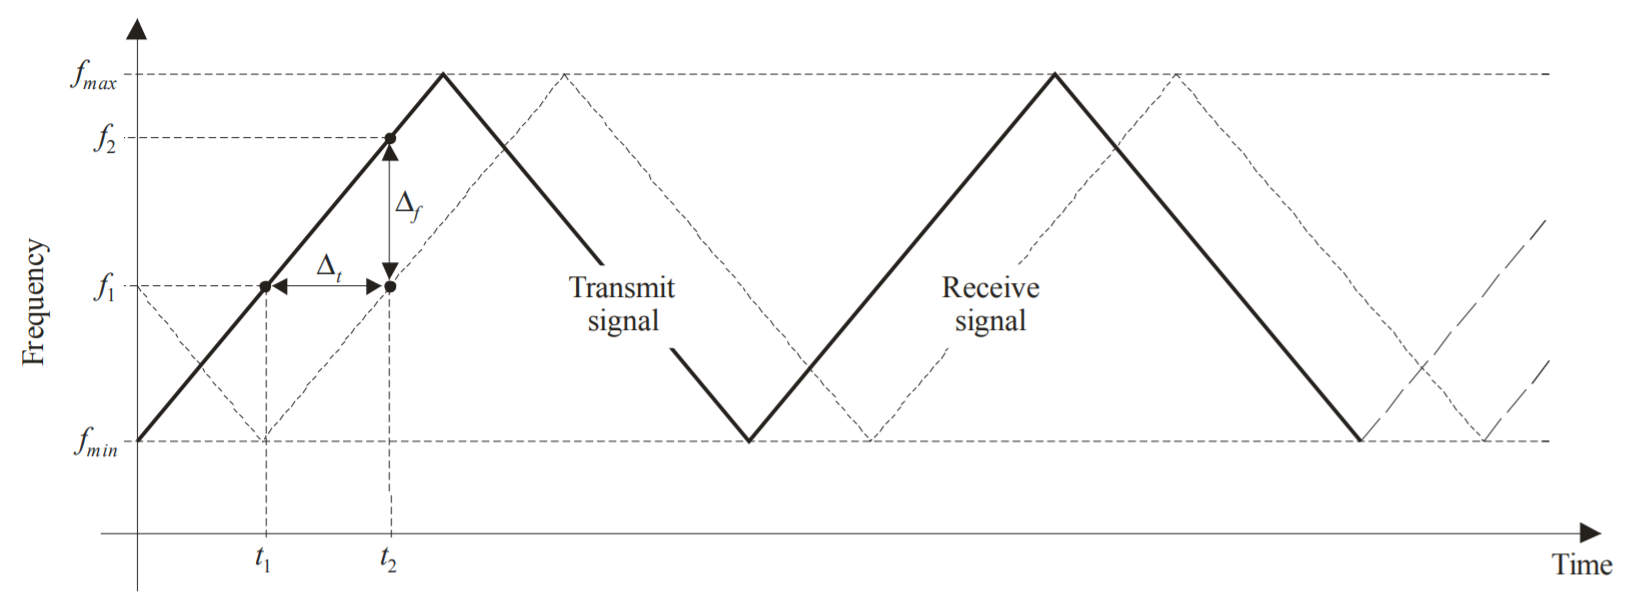
\includegraphics[scale=0.5]{FMCW_Example.PNG}
 \caption{FMCW Waveform from ITU-R M.2059-0 ~\cite{noauthor_operational_2014}}
 \label{fig:FMCW}
\end{figure}
The signal travel time is based on the return of a signal of the same frequency as the transmit signal~\cite{noauthor_operational_2014}. One method for calculating the travel time of a signal involves taking the difference between the frequency of the return signal at the current time and the frequency of the transmit signal at the current time, $\Delta f$. As shown in Figure~\ref{fig:FMCW}, given a constant waveform, the return time of a signal is:

$$\Delta t = \frac{\Delta f}{df/dt}$$

Once $\Delta t$ is calculated, it the height can be determined using the speed of light: 

$$H = \frac{c\Delta t}{2} $$

While not relying on a frequency modulated waveform, pulsed radar altimeters use a series of discrete pulses to track the current height of the aircraft. The $\Delta t$ between two pulses is used to calculate the height in the same manner that an FMCW altimeter does. 

\subsection{Altimeter Signal Processing}
The basic altimeter receiver uses a homodyne detection scheme to extract data from the received waveforms. At an instant in time, the waveform actively being transmitted is sampled and fed into the receiver mixer. All received signals are then down converted to baseband. Newer models apply digital signal processing to the downconverted signal. This is accomplished by applying an FFT to the received signal so that that all processing can be done in the frequency domain. Transformed data is passed to proprietary decision algorithms which perform an altitude estimation. Other altimeters may count the zero crossings of the received signal to determine its frequency~\cite{noauthor_operational_2014}. 

The varying methods of extracting the altitude data make the effects of interference unpredictable. Narrow band signals might cause occasional false readings, while signals spread across the band effectively raise the noise floor of the radar. Digital algorithms which rely on sufficient SNR to function may enter a fail state if the noise floor is raised too much resulting in ``Non Computed Datapoints'' or NCDs~\cite{noauthor_operational_2014}.

\subsection{Radio Altimeter Antennas}
Radio altimeter antennas require a wide half power (3dB) beamwidth to allow the unit to function under all pitch and roll angles performed in flight. The authors of~\cite{noauthor_operational_2014} found no specification for cross pol isolation for altimeter antennas in production, which eliminates a potential method of protecting altimeters from interferers. The authors also found that the necessary orientation of an altimeter antenna toward the ground makes it vulnerable to all posible radiation sources without shielding~\cite{noauthor_operational_2014}.

\subsection{Attenuation of the Altimeter Signal in Free Space}
A signal traveling from Altimeter transmit and back to receive passes through multiple different sources of gain and attenuation. There is attenuation from cable losses, gain from the TX antenna, free space path loss as the signal travels toward the ground, loss from the scattering of the signal by the ground, path loss of the return signal, a gain from the receive antenna, and finally the attenuation from return cable losses. The combination of each of these gains and losses comprises the external loop-loss $L$ for a signal leaving an aircraft. DO-155 operating standard~\cite{noauthor_minimum_1974} defines the loop loss as the ratio of the power received by the RX antenna, $P_R$ to the power sent by the transmit antenna, $P_T$.
$$ L = \frac{P_R}{P_T}$$
The DO-155 standard specifies loop loss for different heights, standardized antennas,  ground scattering environments, and standardized cable attenuations. The standard expands the formula shown here to incorporate these effects~\cite{noauthor_minimum_1974}.
\subsection{Conclusions}
Radio Altimeters are a safety critical system in any aircraft, the output of which is used by other important airborne systems. Altimeters use the time it takes a signal to travel to the ground and back to calculate the height of an aircraft off the ground, and must be able to pick up a return signal which has been attenuated significantly depending on the height. To test radio altimeters in a lab setting, both the time delay and attenuation experienced by a real signal must be simulated. 

%%%%%%%%%%%%%%%%%%%%%%%%%%%%%%%%%%%%%%%%%%%%%%%%%%%
%
%  New template code for TAMU Theses and Dissertations starting Fall 2016.  
%
%
%  Author: Sean Zachary Roberson
%  Version 3.17.09
%  Last Updated: 9/21/2017
%
%%%%%%%%%%%%%%%%%%%%%%%%%%%%%%%%%%%%%%%%%%%%%%%%%%%

%%%%%%%%%%%%%%%%%%%%%%%%%%%%%%%%%%%%%%%%%%%%%%%%%%%%%%%%%%%%%%%%%%%%%%%
%%%                           SECTION II
%%%%%%%%%%%%%%%%%%%%%%%%%%%%%%%%%%%%%%%%%%%%%%%%%%%%%%%%%%%%%%%%%%%%%%


\chapter{METHODS} 
\section{Basic Altimeter Test Bed Setup} \label{sec:Basic}
In addition to laying out performance standards for radar altimeters, the DO-155 standards~\cite{noauthor_minimum_1974} also specify a basic test setup for verifying an altimeter is functioning properly. Figure~\ref{fig:Basic Testbed} shows the diagram of this test setup, which connects the RF terminals of the altimeter to an \textit{altitude simulator} and connects a separate device to read altitude data.  
\begin{figure}[ht]
\centering
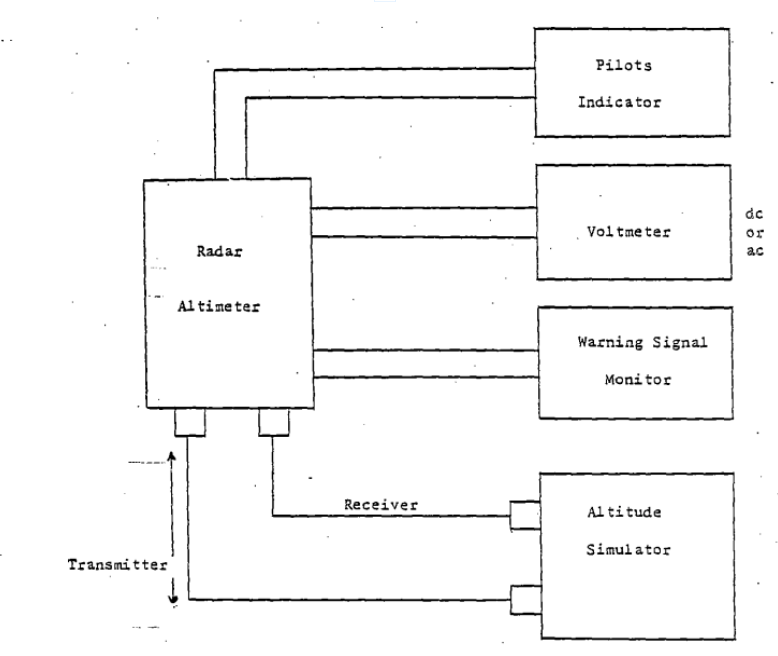
\includegraphics[scale=0.5]{DO-155_Test_Setup.PNG}
\caption{Basic Altimeter Test Setup from DO-155~\cite{noauthor_minimum_1974}}

\label{fig:Basic Testbed}

\end{figure}

The standards elaborated on the necessary characteristics of the most critical part of the testbed, the altitude simulator. The altitude simulator needed to ''consist of variable and fixed RF attenuators''~\cite{noauthor_minimum_1974}  to simulate the loop loss an altimeter experiences aboard an aircraft (see section 1.6.3). The altitude simulator also needed a length of ''coaxial cables or other suitable delays''~\cite{noauthor_minimum_1974}  to simulate the physical time delay experienced by an altimeter signal between the transmitter and receiver (see section 1.6.2). To complete the test setup, the altitude simulator directed the attenuated and delayed RF energy from the transmitter fed back into the receiver. 


Additionally, the standards specified that any test equipment must account for cross coupling between transmitting and receiving antennas. DO-155 emphasized that the altitude simulator should achieve the desired altitude within 1\% and the correct attenuation within 2.5dB~\cite{noauthor_minimum_1974}.

%%%%%%%%%%%%%%%%%%%%%%%%%%%%%%%%%%%%%%%%%%%%%%%%%%%%%%%%%
\section{Modified Altimeter Test Setup} \label{sec:Modified}
AVSI designed a modified version of the altimeter test setup specified by DO-155, shown in Figure~\ref{fig:Modified}. The modifications allow the controlled injection of interference into the line after the altimeter signal passes  through the altitude simulator. 

\begin{figure}[ht]
\centering
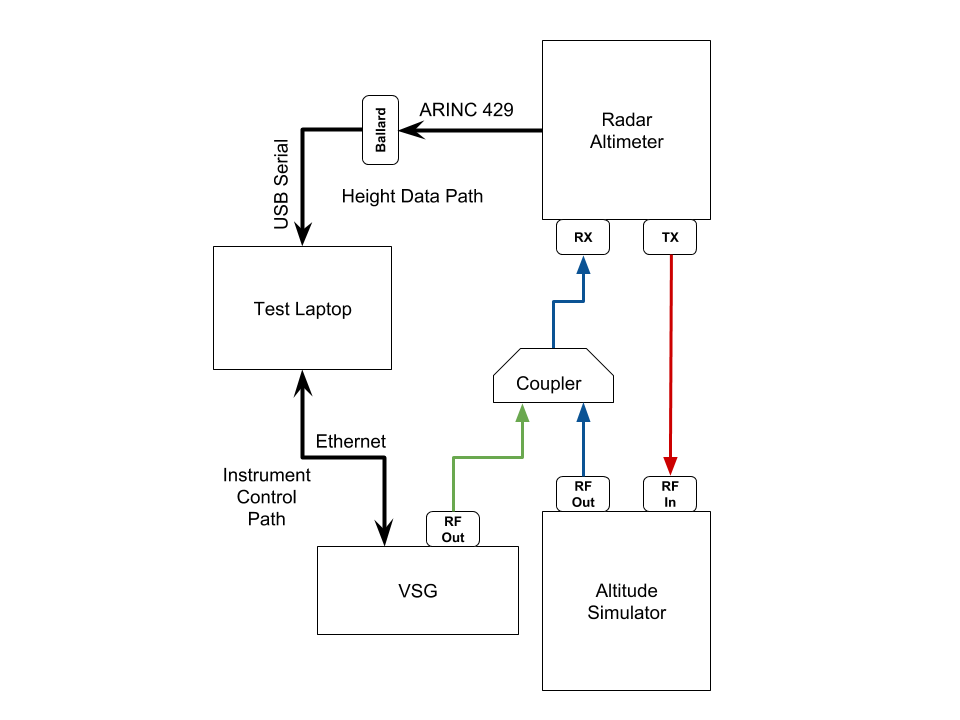
\includegraphics[scale=0.45]{Modified_Test_Setup.png}
\caption{Modified Altimeter Test Setup}

\label{fig:Modified}

\end{figure}
\subsection{Reading the Altimeter Output}\label{sub:reading_out}
The altimeter outputs labeled height data on a standardized ARINC 429 cable configuration. The modified setup uses a Ballard ARINC device to convert the data from ARINC 429 to USB serial format, providing each data point with a time stamp. On the test laptop, Ballard CoPilot software reads the serial data and provides a display which allows the real time monitoring of all altimeter output and labels. 

The labels are critical because some data points may be labeled NCD (No Computed Data) when conditions are insufficient for a reliable height measurement. CoPilot software also allows for the easy export of test data to Microsoft Excel documents for post processing. 
\subsection{Implementing the Altitude Simulator}\label{sub:Implementing}

\begin{figure}[ht]
\centering
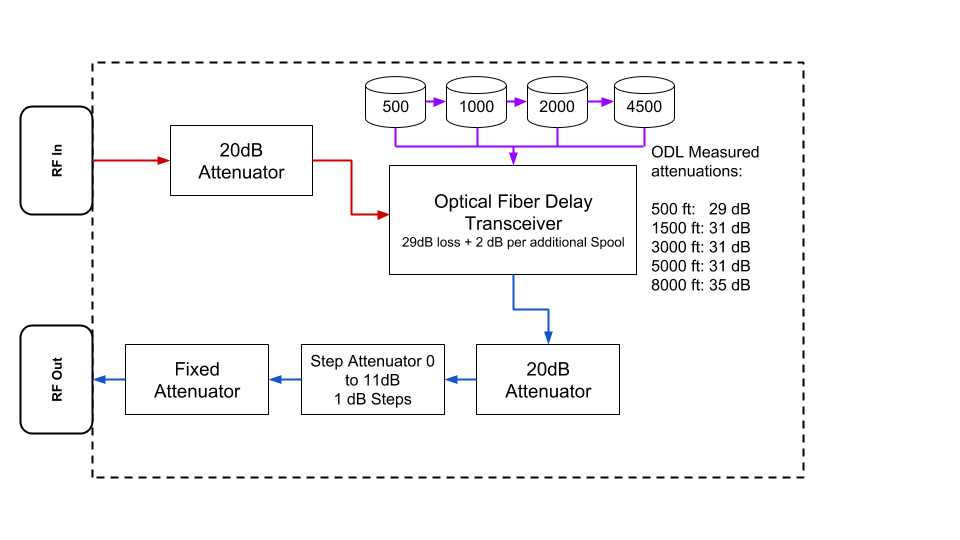
\includegraphics[scale=0.5]{Altitude_Simulator.png}
\caption{Internal Diagram of Altitude Simulator using optical delay line}

\label{fig:Altitude_Simulator}

\end{figure}

\subsubsection{Time Delay}\label{subsub:delay}
Different test altitudes require the use of different methods of delaying the RF energy output by the altimeters. For the initial tests at higher altitudes, spools of fiber optic cables create a time delay as shown in Figure~\ref{fig:Altitude_Simulator}. The RF output from the altimeter transmitter was fed by coax connection to the fiber optic transceiver, which could either pass the signal to a single fiber optic spool or a series of cascaded spools to achieve a desired height. This setup contained optical spools of 500, 1000, 2000, and 4500 feet, each of which could be used individually or in conjunction with any or all of the other spools to implement a delay.

 The optical transceiver and cascaded spools also contribute an attenuation to the loop loss which varies based on the number of spools cascaded. A single spool setup has an attenuation verified experimentally to be 29dB, with an additional 2dB loss added for each additional cascaded spool.

Later tests modified this delay setup to test an altimeter in takeoff and landing scenarios. The much lower height in these scenarios made spools of coax sufficient tor the delay instead of fiber optic cables. Two coax spools provided a height of 40 ft and 95 ft for testing these scenarios, with a 6dB and 36dB attenuation contributed to the loop loss respectively.  

\subsubsection{Achieving Standard Loop Losses}\label{subsub:loss}
DO-155 specifies loop loss for various heights and antenna types. Table~\ref{tab:loop loss} lists the loop loss used for each height in these tests. To achieve the Loop Losses specified by DO-155 standards for each height, the attenuation inherent in the delay method used for each height must be taken into account. 

Once the attenuation from the delay line is subtracted from the loop loss, 10, 20 and 30dB Pasternack fixed attenuators inserted into the setup get within 10dB of the desired loop loss. The first 20dB attenuator is located ahead of the fiber optic transceiver to protect it from damage (see Figure~\ref{fig:Altitude_Simulator}.  Finally, a step attenuator capable of 1 to 11 dB is used to achieve the desired loop loss with a 1 dB precision. 

\begin{table}[]
\centering
\begin{tabular}{|c|c|}
\hline
\textbf{Height} & \textbf{Loop Loss} \\ \hline
40ft            & 76 dB              \\ \hline
95ft            & 84 dB              \\ \hline
500ft           & 100 dB             \\ \hline
1500ft          & 109 dB             \\ \hline
3000ft          & 116 dB             \\ \hline
5000ft          & 120 dB             \\ \hline
8000ft          & 124 dB             \\ \hline
\end{tabular}
\caption{DO-155 Loop Losses}
\label{tab:loop loss}
\end{table}

\subsection{Generating Interference Signals}\label{sub:Generating}
A Rhode and Schwarz SMU200A Vector Signal Generator (VSG) is used to generate simulated WAIC signals of varying modulation types, bandwidths and power levels. The VSG has a SCPI interface which allows an external computer to control any functionality on the instrument through commands sent over either a serial or an Ethernet connection. 
\begin{figure}[ht]
\centering
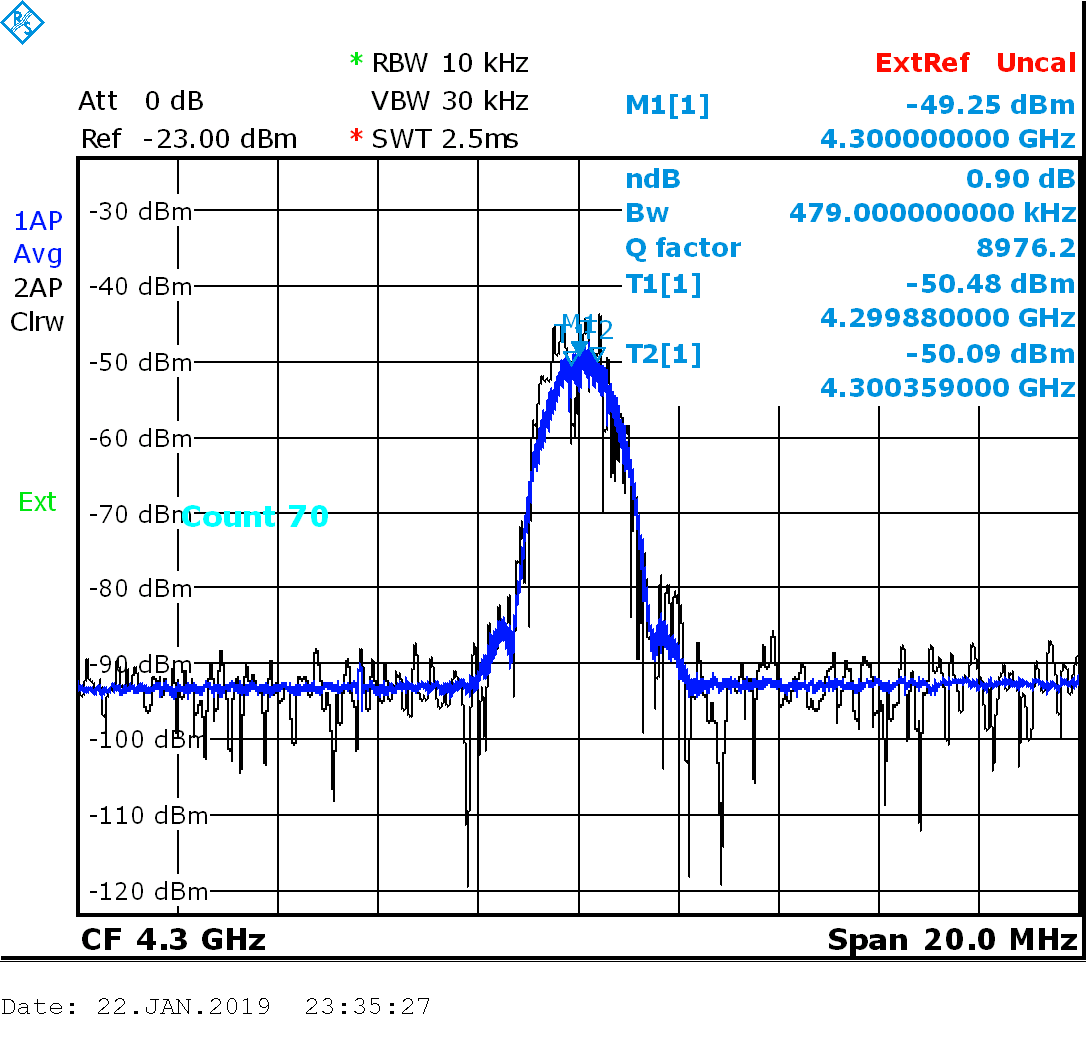
\includegraphics[scale=0.25]{MSK_wvfrm.png}
\caption{MSK Waveform at 4.3 GHz Pictured on a Spectrum Analyzer}

\label{fig:MSK}

\end{figure}

The AFE76 Project Management Committee (PMC) chose the modulation formats to represent candidate WAIC interference. The PMC chose to subject the altimeters to an MSK waveform, as well as OFDM waveforms of varying bandwidths and dual versions of both waveforms. Each waveform used ''junk'' data to modulate the carrier, which consisted of randomly generated ones and zeros with equal probability of either; this closely replicates the performance of an optimized communication system~\cite{unknown}
\subsubsection{MSK Waveform}\label{subsub:MSK}
MSK or Minimum-Shift Keying is a type of modulation format which can be considered as a form of Phase-Shift Keying (PSK) or as a special case of Frequency Shift Keying (FSK)~\cite{proakis_communication_2002}. The frequency separation of an MSK signal, $\Delta f$ is: $$ \Delta f = \frac{1}{2T}$$
and thus it has a modulation index of 1/2. This is ''the minimum frequency separation for orthogonality of the two sinusoids''~\cite{proakis_communication_2002}. An MSK waveform is shown on the spectrum analyzer screen-cap in Figure~\ref{fig:MSK}.

MSK modulation is available natively in the VSG software through the \textit{custom waveform} interface.  The Rhode and Schwarz VSG provides a number of common modulation options in this interface for the user to choose from. This simplifies the waveform generation for this case, as every in-built functionality on the VSG has a SCPI command corresponding to it. 


\subsubsection{OFDM Waveform}\label{subsub:OFDM}

Orthogonal Frequency-Division Multiplexing or OFDM attempts to achieve an efficient, wide-bandwidth communication system by ''dividing the channel bandwidth into equal-bandwidth sub-channels, where the bandwidth of each sub-channel is sufficiently narrow so that the frequency response... of sub-channels are nearly ideal''~\cite{proakis_communication_2002}. An OFDM waveform is shown on the spectrum analyzer screen-cap in Figure~\ref{fig:OFDM}.
\begin{figure}[ht]
\centering
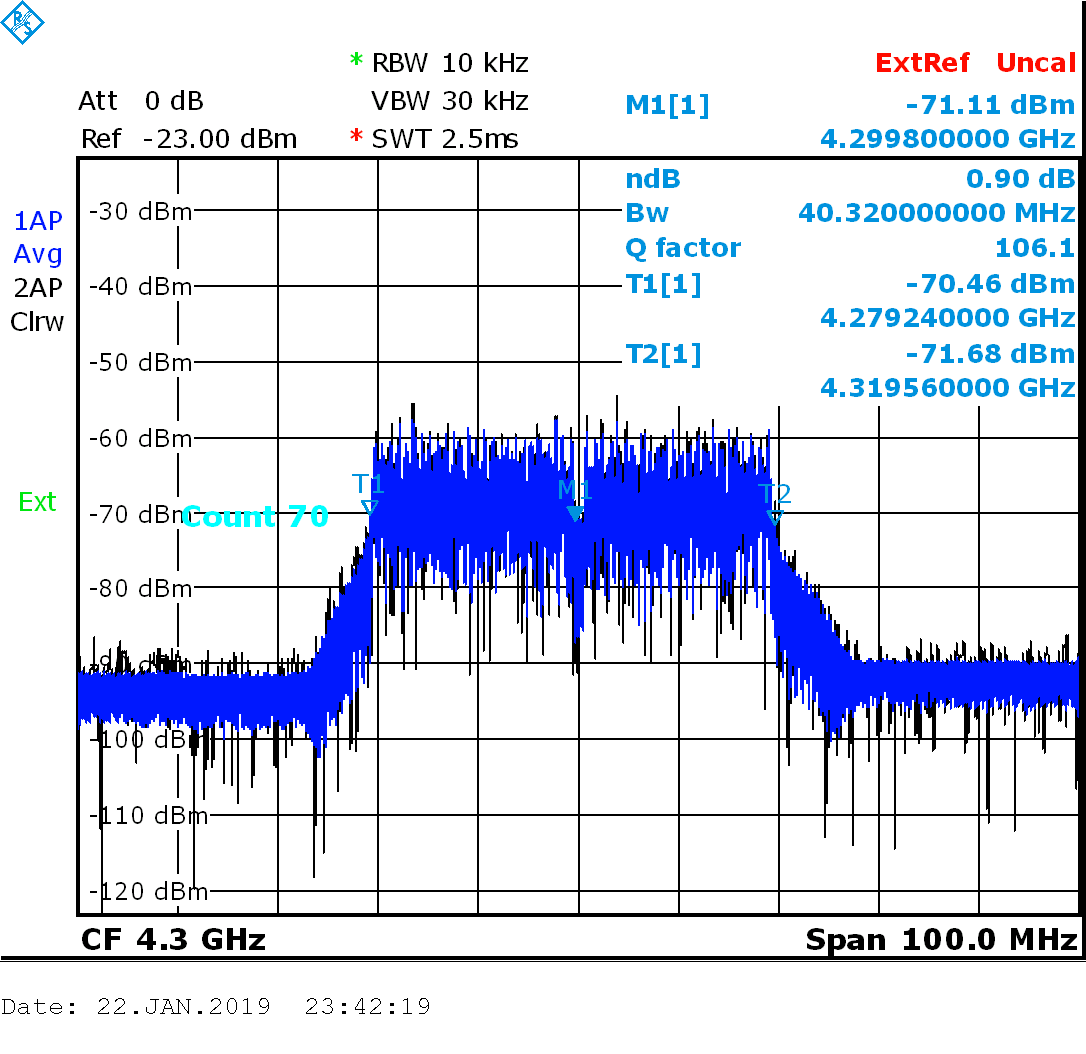
\includegraphics[scale=0.25]{ofdm_wvfrm.png}
\caption{40 MHz OFDM Waveform at 4.3 GHz Pictured on a Spectrum Analyzer}

\label{fig:OFDM}

\end{figure}
One way to view the OFDM waveform is as a series of MSK waveforms spread out orthogonally along a desired bandwidth. From this perspective, MSK can be seen as the minimum bandwidth version of a system based on OFDM, and the altimeter can thus be subjected to wider and wider bandwidth systems to show the response to a greater number of WAIC devices on (or external to) an aircraft. This aspect, as well as the similarity of an OFDM signal to LTE systems made it a very attractive option for testing the impact of WAIC. 

Generating OFDM signals with the VSG was a more involved process than generating MSK, because the functionality for creating OFDM was not available natively in the VSG software. Because of this, OFDM had to be generated through the VSG's \textit{Arbitrary Waveform Generator}. The arbitrary waveform generator enables the VSG to generate any waveform from IQ data stored in a file on the VSG. The SCPI command for generating an arbitrary waveform must include the file path for this IQ data.  

This enabled an OFDM waveform to be specified by a Matlab script which exports raw IQ data, which is then converted to a form readable by the VSG through proprietary Rhode and Schwarz software. The conversion software allowed the user to adjust the clock rate, thus adjusting the bandwidth of the signal used. The bandwidth could then be measured with a spectrum analyzer to verify the process has yielded the expected waveform. The bandwidth of the OFDM waveform was defined as being 6 dB down from the peak envelope power. 


\subsubsection{Dual Waveforms}\label{subsub:Dual}
The VSG allows full control of an RF generator along with two baseband generators. The RF generator gives the user control of RF carrier frequency as well as the output power level of the carrier in dBm. The baseband generators allow the modulation of two potentially unique waveforms onto the carrier wave, with a possible offset frequency from the center. Both dual MSK waveforms and dual OFDM waveforms of bandwidth less than 40 MHz were tested using a +/-20 MHz offset between them. 

Dual waveforms were considered an important option for testing due to a special characteristic of some altimeters at low altitudes. As the plane descends, the sweep rate of an altimeter increases to give more frequent readings at a more safety critical phase of flight. This is done by significantly reducing the $\Delta f$ covered by the altimeter FMCW. The effects of this offset were thus investigated to determine whether WAIC's impact could be minimized at critical altitudes by leaving the center of the band clear. 


%%%%%%%%%%%%%%%%%%%%%%%%%%%%%%%%%%%%%%%%%%%%%%%%%%%%%%%%%
\section{Python Test Software}\label{sec:Python}
Python code written by the author pieces together the various parts of this setup into an integrated test bench. Different Python scripts control the various functions of the test bench. These include:

\begin{itemize}
\item Creating a database to transfer data between different Python Scripts
\item Interface with the VSG to generate interference signals
\item Parse the CoPilot log
\item Mapping time stamped height measurements to time stamped interference signals
\item Plotting and analyzing the results
\end{itemize}

\begin{figure}[ht]
\centering
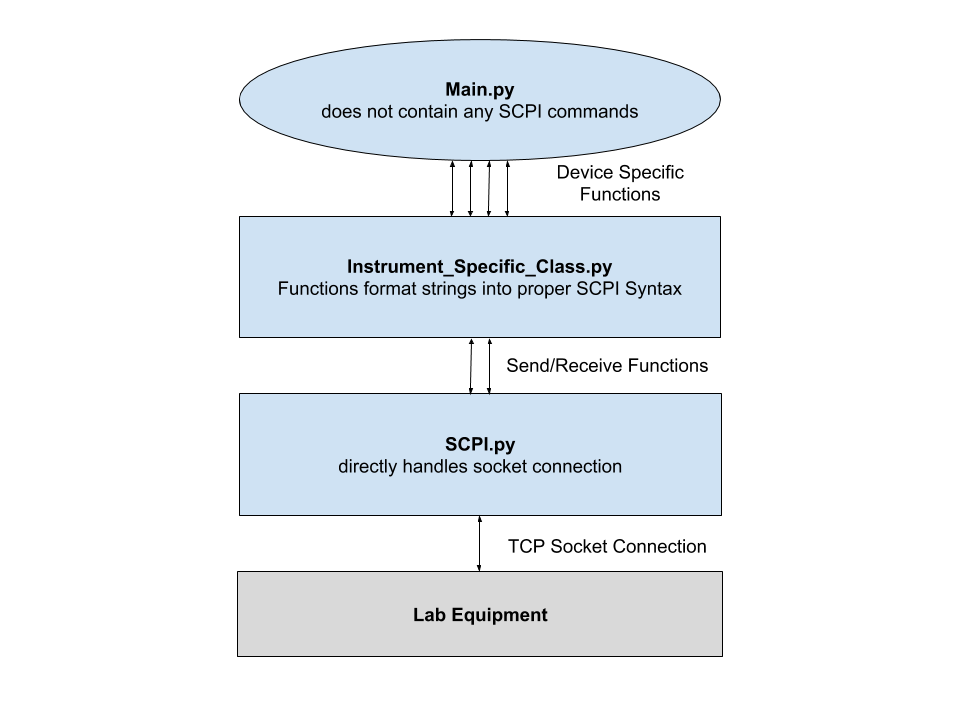
\includegraphics[scale=0.45]{SCPI_Class_Hierarchy.png}
\caption{SCPI Class Hierarchy}

\label{fig:SCPI}

\end{figure}
The software uses Standard Commands for Programmable Instruments or SCPI to control the vector signal generator. In this test bed, the SCPI instructions are processed through an object-oriented hierarchy shown in Figure~\ref{fig:SCPI}. The super-class, $SCPI$ interfaces directly with all lab equipment. The subclass, called \textit{RS\_Signal\_Generator} in this implementation, contains Python functions associated with all instrument specific commands. The helper functions from $SCPI$ send and receive communication with the instrument. Finally, the main loop exists at the highest level, which times the calls of different instrument commands and creates a database to store them. The idea behind this abstraction is to prevent the main loop from dealing with any raw SCPI command syntax-- this should only be handled by one of the instrument classes. 



\subsection{Test Main Loop}\label{sub:mainloop}
The highest level of this design is the test main loop. The test main loop creates the SQLite database which stores all important information for easy transfer between the different python scripts necessary for the test bed. This program also contains variables for various test parameters, which are stored in an SQLite database for easy reference and sometimes directly control the sequence of a test. Finally, this program loops through the sequence interference signals specified by the various test parameters, and sends the commands to the VSG to generate them. The commands sent to the VSG are time stamped as precisely as possible, and recorded in the \textit{Generated Signals} table in the database. 


Certain test parameters are stored for reference or calculation but do not directly affect the sequence of interference signals to be generated. These include the altimeter make and model, the nominal height of the test setup, the loss experienced by interference signals traveling to the altimeter RX, and the loop loss used in the setup. Other parameters directly control the sequence of the test, including interference on and off times, power levels to be used, modulation formats to be tested, and RF carrier frequencies to be used. 

\subsubsection{Nominal Height vs Correct Height}\label{subsub:nominal}
\textit{Nominal height} is the term used to refer to the approximate altitude determined by the experimental test setup. The difference between measured height and the nominal height of the setup varies between the different altimeters, and is primarily a result of different calibration settings for each altimeter. The calibration procedure is an important part of installing an altimeter onto an aircraft. When an aircraft is on the ground, the TX and RX antennas used by the altimeter are naturally several feet off the ground, in line with the airframe. Additionally, there are standardized delays from the altimeter TX port to the TX antenna and from the RX antenna to the RX port. These are known as Aircraft Internal Delays (AIDs). To compensate for the varying heights of airframes, as well as the AID installation, avionics manufacturers developed a calibration procedure so that each altimeter could be programmed upon installation to output an altitude of 0ft when the plane is on the ground. 

Because these tests are only concerned with a differential \textit{height error}, rather than the accuracy of an absolute altitude measurement, \textit{nominal height} is only used to set the loop loss. Instead, the baseline measured height with no interference, or \textit{correct height}, is calculated in post processing as the median altitude over a several minute period when the VSG is in the OFF state before the test begins. Any height error attributable to interference is measured as a distortion from this correct height. Because of this, calibration of each altimeter to the setup is unnecessary. 

\subsubsection{Sequence Control}\label{subsub:sequence}
% This section also needs a plot to show the timed stepping up of interference signals. 
The primary purpose of the test main loop is to subject an altimeter to various modulation formats, gradually stepping up the power of each until the altitude readings from an altimeter are distorted or broken. The main loop determines the type of modulation, power level, and timing, and as each signal is turned on or off by the VSG, stores the parameters for the signal in the \textit{Interference Signals} table for use in post processing, an example of which is shown in Table ~\ref{tab:Interference}. Each unique modulation format and power combination will have two entries in the \textit{Interference Signals} table, corresponding to the RF ON and RF OFF states of the VSG.  
\begin{table}[]
\centering
\begin{tabular}{@{}cccccccc@{}}
\toprule
ID & Altimeter   & Start Time          & End Time            & Modulation &Carrier Freq& Power & RF State \\ \midrule
1  & Alt A & 19:23:06 & 19:23:07 & MSK & 4300  MHz & -10  dBm & OFF      \\
2  & Alt A & 19:23:07 & 19:23:08 & MSK & 4300   MHz & -10 dBm& ON       \\ \bottomrule
\end{tabular}
\caption{Example Interference Signal}
\label{tab:Interference}
\end{table}

A variety of parameters controls the progression of different interference signals. The \textit{interference\_duration} and \textit{signal\_off\_duration}, define the length of time the altimeter will be subjected to a particular interference signal, as well as the length of time the altimeter will have to recover from any error caused by the previous signal. Throughout the main loop, each signal's Start Time and End time is calculated using interference duration variables. 

 A range of RF powers is specified using \textit{power\_min}, \textit{power\_max}, and \textit{power\_step}. For a given modulation format, the main loop iterates through each power level in this range, subjecting the altimeter to this interference power. This allows the user to step through increasing power with as much granularity as is desired for the test


The final variable which is important to the progression of a test is a list called \textit{modulation\_formats}, which contains strings corresponding to the different modulations the VSG will generate. MSK and OFDM signals of varying bandwidths will be listed here. The main loop iterates through each string in this list, passing the string to helper functions. 

The first helper function is a lookup which calls the proper function in the VSG class corresponding to a specific modulation format string. The second helper function gives the option for different modulation formats to be put on different carriers, or a list of different carrier functions. Iterating through different carriers for different modulation formats proved to be a critical functionality in later tests.

\subsubsection{Precision of Timing Commands}\label{subsub:timing}
During initial tests of the main loop, problems occurred which prevented the \textit{interference\_duration} and \textit{signal\_off\_duration} from precisely controlling the duration and recovery time of an interference signal. This section provides an overview of the different timing issues encountered over the course of these tests, as well as the approaches taken to mitigate each issue. 
 
The first and most serious issue encountered while running these tests were termed \textit{hanging delays}. These occurred when the main loop progressed more or less as expected, but the vector signal generator would ''hang'' in its previous state for a significant period of time after the command was sent. 



% Please add the following required packages to your document preamble:
% \usepackage{booktabs}
\begin{table}[]
\centering
\begin{tabular}{@{}ccccccccc@{}}
\toprule
ID & Timestamp   & RF State & Power  & PEP  & Carrier  & Offset 1 & Custom 1 & Arb 1 \\ \midrule
1  & 11:49:39.96 & 1        & -3 dBm & 4.48 & 4300 MHz & 0        & 0        & 1     \\
2  & 12:09:40.26 & 0        & -3 dBm & 4.48 & 4300 MHz & 0        & 0        & 1     \\ \bottomrule


\end{tabular}
\caption{Example VSG State Table}
\label{tab:VSG_State}
\end{table}
 
	 First, the program was modified and a new table was added to the database to store the Vector Signal Generator state after each set of commands. Since the purpose of this table was only to be used for debugging, entries were kept as simple as possible. For example, a $1$ in \textit{RF State} corresponds to RF ON, while conversely a $0$ in \textit{RF State} corresponds to the RF OFF setting. The \textit{Power} and \textit{Carrier} columns correspond with the same values in Table~\ref{tab:Interference}. \textit{Offset 1}, \textit{Custom 1}, and \textit{Arb 1} correspond to the state of the first Baseband generator, telling whether the \textit{Custom Waveform Generator} corresponding to a MSK Waveform (see Section~\ref{subsub:MSK}) or the \textit{Arbitrary Waveform Generator}(see Section~\ref{subsub:OFDM}) corresponding to an OFDM waveform are active respectively. 
	 
For the purposes of the timing problem, these attributes serve as a fingerprint, allowing an investigator to correlate each row in the VSG State Table to a row in the Interference Signals table. While information here may seem redundant, this value differs notably from the values in the interference signals table in that the VSG state table is only populated \textit{with values received from the Vector Signal Generator}. Because of this, this table allows for a simple method for looking through the data to find at which point the VSG might ''hang'' in its current state rather than switch to the next signal as specified in the interference signals table. 

Using this method, different theories for potential causes of the hanging delays were investigated. The first potential problem was dropped or delayed packets. During the initial setup, instruments were connected to one another over the TAMU network. While this functioned at a high level, upon packets had an unnecessarily long mean travel time, and significant outliers existed during times of heavy traffic. These issues were solved by moving the VSG and controller laptop onto their own local network. 

 While the local network solved the biggest chunk of hanging delays, it did not eliminate them entirely. These were attributed to a slowdown in the processor handling the sequence of Python commands.These remaining delays would only occur at times of extremely heavy CPU usage (possibly caused by a memory leak in the old Ballard driver), and were eliminated almost completely by rebooting the controller laptop more frequently. Later on, an upgrade to the Ballard driver reduced these even further. 
 
 While the hanging delays were investigated, the VSG State table revealed another source of imprecision in timing commands. It was noticed that the VSG State would not change until nearly a second longer than the \textit{Interference Duration} or \textit{Signal off Duration} parameters specified. This drift occurred because the main loop used Pythons in built \textit{Sleep()} function to handle timing. The sleep function used the exact interference duration passed as a parameter. After the program 'woke up' the commands to set the next interference signal up would be called, thus introducing a small delay beyond the specified duration. 
 
 This problem was dealt with by replacing the \textit{Sleep()} function with a custom function called \textit{Wait\_Until()}. This new function takes the signal end time as a parameter (See Table ~\ref{tab:Interference}), subtracts the current time from the end time, and uses the new value as the parameter for Python's in-built sleep function. This allows the next end time to be calculated in advance by adding the \textit{Interference Duration} or \textit{Signal off Duration} to the previous signal's end time, and storing the previous signal's end time as the start time for the next signal. %[This section definitely could use some sort of diagram...]

Using the \textit{wait until} method to time commands offered important new flexibility to the main loop. This method allows writing signals to a database, setting up the baseband generators, and pinging the VSG for the VSG State information all to occur while the VSG is in an RF OFF state. While the VSG settings can not be adjusted in RF ON while maintaining the integrity of the signal, writing to the database and pinging the VSG for state information can also be done during this state, and the \textit{wait until} function will still wake the program at the proper time to turn the VSG on or off. The implementation of the \textit{wait until} function eliminated the drift problem, and allowed for the \textit{Interference Duration} and \textit{Signal Off Duration} parameters to precisely control the signal on and off time. 

\begin{figure}[ht]
\centering
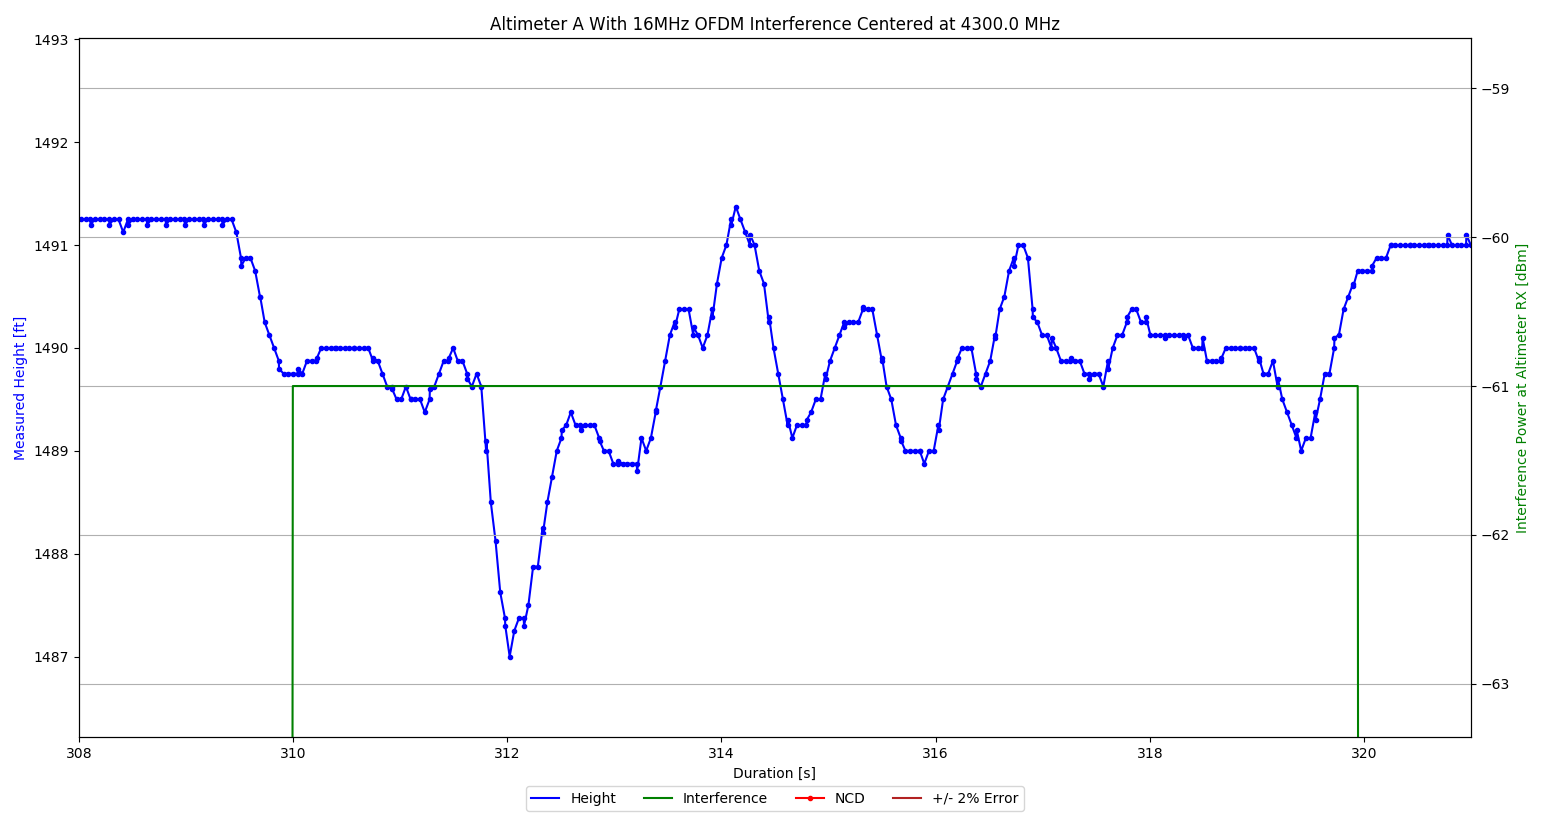
\includegraphics[scale=0.65]{sync_err.PNG}
\caption{Height Plot Showing Sync Error}

\label{fig:sync}

\end{figure}
The final problem encountered involved the synchronization of time stamps of data between the controller laptop and the Ballard ARINC device. The Ballard internal clock drifted from about half a second ahead of the controller laptop clock to about half a second behind. This led to data sets such which looked like Figure~\ref{fig:sync}, where distortion from the correct height would appear a split second before the interference signal was turned on. Additionally, due to averaging techniques used in the altimeter's signal processing, there would be several data points during which the altitude would recover from the distortion caused by any interference. 


While this issue could not be fixed completely, several different approaches were taken to mitigate it. Firstly, the Ballard used in initial testing was an older unit, which meant it was more prone to clock errors. To address this, the clock was driven by an external IRIG-B timecode signal, rather than the on board IRIG~\cite{noauthor_overview_2017}. A program called NMEA time generated the IRIG signal through the controller laptop's audio jack, which was then fed into the Ballard input.  These changes would not completely synchronize the Ballard, but it would limit the drift of one clock away from another throughout a test. 


Later on, when a new Ballard was purchased for this project, the external IRIG signal was no longer needed, as the updated Ballard driver provided adequate synchronization over USB. Another technique used to prevent any loss of synchronization was to periodically power cycle the Ballard to ensure that the clock is reset. Finally, to minimize the impact of any data points not captured in the RF ON interval by post processing, long interference durations were used to ensure that the impact of any missed points on the true average was minimized. 

\subsection{VSG Class}
The VSG Class allows the main loop to create an object corresponding to each VSG connected to the network in the lab setup. This object then has access to functions which perform every operation needed by the main loop. The VSG Class inherits functionality from \textit{SCPI.py} common to every SCPI programmable instrument. The VSG class provides functionality for controlling both the RF generator, as well as the VSG's two baseband generators. 

The general purpose of each function in the VSG class is to construct the string for each SCPI command corresponding to that function, and send the command using the inherited SCPI \textit{send} function. For example, the following SCPI command sets Baseband A to MSK modulation:
{\centering\textit{''SOUR1:BB:DM:FORM	MSK''}\par}
''SOUR1'' corresponds to baseband generator A, where ''SOUR2'' would correspond to baseband generator B. Different SCPI commands have different parameters like this which the VSG class takes in as a normal Python variable and inserts into the string. 

The VSG class provides several functions which perform this task for the RF Generator. RF ON and RF OFF commands are self explanatory, while the \textit{set\_carrier} function lets the user choose a carrier frequency as well as the RF power setting.

Similarly, the VSG class offers functions which will set the custom modulation format of either baseband generator (for setting MSK), or for setting the arbitrary waveform generator in each baseband generator (for setting OFDM).This class also provides functions for enabling and disabling the baseband generators, which is necessary for switching between dual and single modulation formats. 

Lastly, the VSG class will have functions for setting a dual MSK or dual OFDM waveform. These will make two calls to the single MSK or OFDM function within VSG, simply passing a different source parameter to specify a different baseband generator.  
\subsection{SCPI Class}
\textit{SCPI.py} contains the 'lowest' level of programming in the SCPI hierarchy shown in Figure~\ref{fig:SCPI}. The goal of this abstraction was to implement a small set of core functionality that would be needed for any instrument capable of running SCPI commands. The SCPI class handles the TCP connection, sends and receives all commands and queried data from the instrument, and contains a few other universal instrument commands. 

The first task handled by SCPI is the initialization of the socket connection between the controller laptop and the instrument. The constructor takes in the IP address of the instrument and the port number, and uses the Python socket class to initialize the connection. When the experiment is over, the SCPI \textit{close} function which handles the proper termination of the socket connection. 

Next, the SCPI class creates custom send and receive commands inherited by every instrument object. The send command handles the proper encoding of any SCPI command string before calling the native socket class \textit{send} function. The receive command decodes a received string from the instrument, and parses the string into the different array elements delimited by commas in SCPI syntax. The receive command is meant to be called within any subclass command which \textit{queries} the instrument for information, as the data types received will vary depending on the query. 

Finally, there are a few other commands universal to almost every SCPI controlled device. The \textit{reset} command ensures the instrument begins each experiment from a clean state. The \textit{operation complete} query is called between commands to ensure that no commands are executed out of order. Last, the \textit{identify} query returns the instrument make and model information, which is useful when first setting up an instrument for automation. 

\subsection{Post - Processing}
After the test sequence is completed, a series of other Python scripts are used to post process the newly generated data. Time stamped altitudes must be exported from the Ballard CoPilot software into an Excel document, and a python script has to read the data from this log into the SQLite database. A second program uses the time stamps from both the logged altitude table and the generated signals table to create a full data set, where each altitude measurement is labeled with the type and magnitude of interference the altimeter was subjected to at that time. Finally, several Python scripts take this full dataset and use it to generate plots which aid in the interpreting of the results. 
\subsubsection{Parsing The Copilot Log}
The first post processing script parses the Ballard Copilot log into the SQLite database so that it can be used by other scripts. The CoPilot export is in an excel file formatted like Table~\ref{tab:Copilot}. This table is read by python using SQLite's built in \textit{read\_excel} function. Most of the data is then added to the SQLite database as is, but the \textit{Value} string is stripped of units and cast as a float so that the numerical value can be easily used by other scripts. 

The most important columns are the \textit{Value}, \textit{Time}, and \textit{Activity} label. The Activity label reads 'SSM ERROR'  whenever the altimeter does not receive a strong enough signal to make a reliable altitude calculation. Points with this flag are called NCD or Non-Computed Data. 
\begin{table}[]
\centering
\begin{tabular}{ccccccc}

\hline
Item \# & Ch\# & Lbl\# & Value    & Time    & Activity      & Name         \\ \hline
0       & 0    & 165   & 509 feet & 26:45.4 & LO            & Radio Height \\
1       & 0    & 165   & 509 feet & 26:45.5 & LO SSM ERROR & Radio Height \\ \hline
\end{tabular}
\caption{Example Copilot Export}
\label{tab:Copilot}
\end{table}
\subsubsection{Mapping Interference Signals to Copilot Data}
The next post processing script maps each of the Altitude data points from the copilot log (Table~\ref{tab:Copilot}), and maps them to the interference signal (Table~\ref{tab:Interference}) active at that time. The method for mapping them is simple: if the time stamp for the data point is greater than an interference signal's \textit{start time} and less than the same interference signal's \textit{end point}, the altitude data is labeled with the corresponding modulation format, RF Power, RF State, and Altimeter under test information from the interference signals table. This process is repeated until all data points have been mapped. 

% Please add the following required packages to your document preamble:
% \usepackage{booktabs}
\begin{table}[]
\centering
\begin{tabular}{@{}ccccccclll@{}}

\toprule
ID & Timestamp  & Ch\# & Carrier& Altimeter & Height & Modulation  & Power& Status & RF \\ \midrule
0  & 13:54:40.5 & 0    & 4300              & Alt A     & 506             & 80 MHz OFDM & 7               & LO     & ON       \\
1  & 13:54:40.6 & 0    & 4300              & Alt A     & 506             & 80 MHz OFDM & 9               & LO     & OFF      \\ \bottomrule
\end{tabular}
\caption{Example Full Dataset Table}
\label{tab:Full}
\end{table}

%%%%%%%%%%%%%%%%%%%%%%%%%%%%%%%%%%%%%%%%%%%%%%%%%%%%%%%%%
\section{Initial `Waic Only' Test Plan}\label{sec:initial}
The test setup design described above gave a wide degree of flexibility to the type, magnitude, and timing of interference the altimeters could be subjected to. While some preliminary tests helped to develop and debug the test setup, these were not comprehensive enough to draw conclusions from. This covers the development questions of for and the execution of the first  comprehensive test regimen. Additionally, this section pieces together the components discussed earlier into a complete test diagram. 

\subsection{Motivations}
The initial testing regimen had a series of questions about the behavior of real altimeters in the presence of interference that needed to be answered: 

\begin{itemize}
\item At what power level will \textit{any} MSK or OFDM signal at 4.3 GHz `break' an altimeter?
\item Does the 'breaking point' an altimeter depend on the bandwidth of the signal?
\item Does adding separation between interference signals at the center influence the `breaking point'? 
\item How does the positioning of a signal within the altimeter band affect the breaking point?
\item The \textit{definition} of precisely what `breaking point' means in the context of these tests also needed development.  
\end{itemize}

A discussion of preliminary testing between the PMC and the author in the context of these driving motivations led to development of the methods discussed in earlier sections which culminated in the test procedure discussed here.  

\subsection{Complete Diagram}
While the diagram of the Modified Test Setup in Figure~\ref{fig:Modified} gives conceptual background to the tests, and Figure~\ref{fig:Altitude_Simulator} gives detailed insight into the operation and configuration of the altitude simulator, neither is detailed enough to provide the context necessary for a complete test description. Figure~\ref{fig:Initial} shows the full test setup used in detail. A full page version is provided in Appendix 1. 




\begin{figure}[ht]
\centering
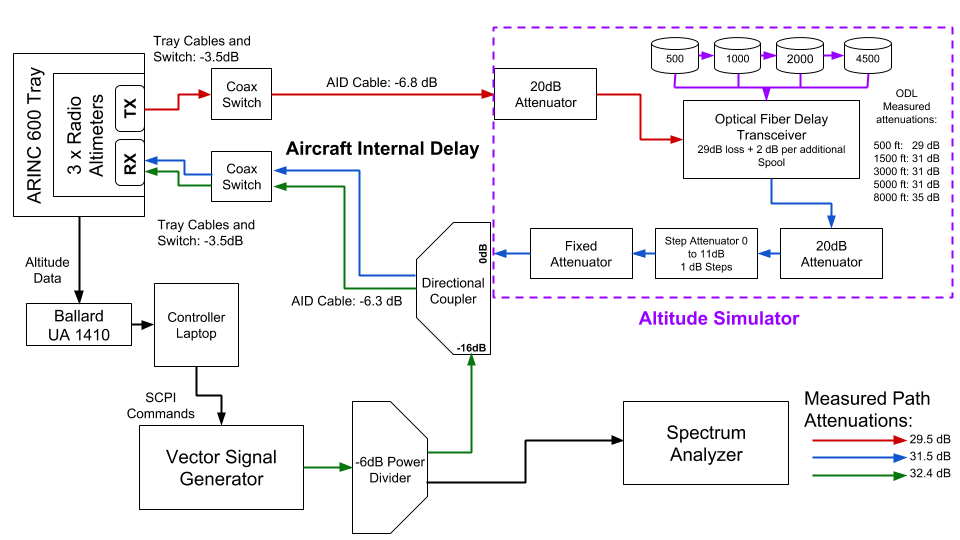
\includegraphics[scale=0.5]{Initial_Full_Setup.PNG}
\caption{Full Test Bench Diagram for Initial Tests}

\label{fig:Initial}

\end{figure}


This diagram shows the altitude simulator  embedded into the full test setup, as well as measured path attenuations with the step and fixed attenuation set to zero. The measured path attenuations are then used to determine a value for the fixed attenuator (10,20, or 30dB), and a value for the step attenuator (1-11dB) to precisely achieve the DO-155 specified loop loss between TX and RX. Table~\ref{tab:loop loss} shows the loop loss values used for the different heights in this setup. 

For 500ft, which had the lowest attenuation, the loop loss from TX to RX was just within the dynamic range of a network analyzer, and so could be verified experimentally with a single S21 measurement. Higher altitudes could not be verified in this manner, but because the measurement closely matched calculations for 500ft, extrapolating to higher altitudes and loop losses was reasonable. 

Several elements not shown in the conceptual diagram from Figure~\ref{fig:Modified} are added in Figure~\ref{fig:Initial}. The output of the VSG is divided between the interference injection point and a spectrum analyzer using a 6dB resistive coupler. The spectrum analyzer allows the test operator to view the interference signals actively being tested, and make adjustments to the setup when they don't match expectations. A directional coupler allows interference to be inserted into the altimeter line at the injection point without adding additional attenuation to the loop. 

 Other elements pictured which weren't on the original diagram include coax switches and an ARINC 600 tray. The tray and switches are necessary in part because the DC power supply to each altimeter is different, and the tray acts as a protection from damage. Additionally, they allow for quick and easy alternating between the various altimeters under test, which is important in case any of this is ever actually flight tested. 
\subsection{Breaking Point Definition}

The purpose of these tests was to search for an altimeter's `breaking point' under various scenarios of interference. Performance standards for radio altimeters first set out in DO-155 were updated in the ARINC 707 standards~\cite{noauthor_arinc_2009}. The standards stated that ``radio altimeter accuracy, when measured in accordance with RTCA DO-155, [should] be within 1.5 feet or 2\%, whichever is greater.''  WAIC or out of band interference needed to demonstrate that it distorted the altitude signal less than these standards. Thus, the breaking point was defined as either a) a maximum height error beyond the 2\% or 1.5 feet allowable by ARINC 707, or b) any height reading labeled NCD. 

\subsection{Test Definition}
\begin{table}[]
\begin{tabular}{c|c|c|c|c|c|c|c|c}
\multicolumn{4}{c|}{\textbf{Interference Signal}}   & \multicolumn{3}{c|}{\textbf{VSG RF Power}} & \multicolumn{2}{c}{\textbf{Power Durations}} \\
Modulation & Bandwidth & Center   & Offset & Min         & Step    & Max       & ON                & OFF              \\ \hline
MSK        & 5 MHz     & 4300 MHz & 0 MHz  & -60 dBm     & 2 dB    & 10 dBm    & 10 s              & 10 s             \\
Dual MSK   & 5 MHz     & 4300 MHz & 20 MHz & -60 dBm     & 2 dB    & 10 dBm    & 10 s              & 10 s             \\ \hline
OFDM       & 5 MHz     & 4300 MHz & 0 MHz  & -60 dBm     & 2 dB    & 10 dBm    & 10 s              & 10 s             \\
Dual OFDM  & 5 MHz     & 4300 MHz & 20 MHz & -60 dBm     & 2 dB    & 10 dBm    & 10 s              & 10 s             \\ \hline
OFDM       & 10 MHz    & 4300 MHz & 0 MHz  & -60 dBm     & 2 dB    & 10 dBm    & 10 s              & 10 s             \\
Dual OFDM  & 10 MHz    & 4300 MHz & 20 MHz & -60 dBm     & 2 dB    & 10 dBm    & 10 s              & 10 s             \\ \hline
OFDM       & 20 MHz    & 4300 MHz & 0 MHz  & -60 dBm     & 2 dB    & 10 dBm    & 10 s              & 10 s             \\
Dual OFDM  & 20 MHz    & 4300 MHz & 20 MHz & -60 dBm     & 2 dB    & 10 dBm    & 10 s              & 10 s             \\ \hline
OFDM       & 40 MHz    & 4300 MHz & 0 MHz  & -60 dBm     & 2 dB    & 10 dBm    & 10 s              & 10 s             \\
OFDM       & 80 MHz    & 4300 MHz & 0 MHz  & -60 dBm     & 2 dB    & 10 dBm    & 10 s              & 10 s            
\end{tabular}
\caption{Test Definition For Initial Testing Regimen}
\label{tab:initial_signals}


\end{table}
Table~\ref{tab:initial_signals} shows the interference signals used for one of the last runs of the initial testing regimen. This test definition was the result of a year and a half long process of expirimentation with the test setup.Tests expirimented with loop loss settings, investigated the ARINC429 synchronization issues, investigated the relative sensitivity of different portions of the band, and investigated the bandwidth dependence of interference signals. The results of the earlier tests are summarized here, while the test definition from Table~\ref{tab:initial_signals} is used as a representative example. 

Early tests experimented with the position from which loop loss was to be measured. There was an argument that the loop loss should be measured between the terminals of the altitude simulator rather than the terminals of each altimeter. This was abandoned when multiple altimeters were unable to acquire an altitude signal with the higher loop loss. This led to the values from Table~\ref{tab:loop loss} of attenuation between altimeter terminals being finalized. Investigations into the measurement syncronization issue were covered in depth in Section~\ref{subsub:timing}.

 Another early test procedure investigated which portion of the radio altimeter band was most sensitive to interference. OFDM signals of the same bandwidth were placed at varying center frequencies to test the altimeters' sensitivity to band placement. These tests confirmed the hypothesis that the center of the radio altimeter band was the most sensitive to interfering signals. 

Finally, the test regimen shown in Table~\ref{tab:initial_signals} was used to systematically investigate the sensitivity of the radio altimeters to different bandwidths of interference. These signals were used across all altimeters under test, and across all altitudes the optical delay line could produce in Table~\ref{tab:loop loss}. The results are discussed in Section~\ref{sec:initial_results}.

%%%%%%%%%%%%%%%%%%%%%%%%%%%%%%%%%%%%%%%%%%%%%%%%%%%%%%%%%
\section{Expanding the Test Setup}\label{sec:expanding}
The results from the initial test regimen led to new avenues of investigation. The dependence of results upon the bandwidth occupied by interference signals led to a need for wider bandwidth signals in the test bed. A desire to present the worst possible case for an aircraft led to testing at lower altitudes with interference from other altimeters. This simulated an approach or takeoff scenario at a busy airport. Finally, developments in 5G communications lobbying for access to adjacent bands led to an investigation of the tolerance of real altimeters to out of band interference. All of this required modifications to the initial testing concept from Figure~\ref{fig:Modified} to couple in an extra VSG and simulated altimeter signals at the interference injection point (Figure ~\ref{fig:Wideband}).
\begin{figure}[ht]
\centering

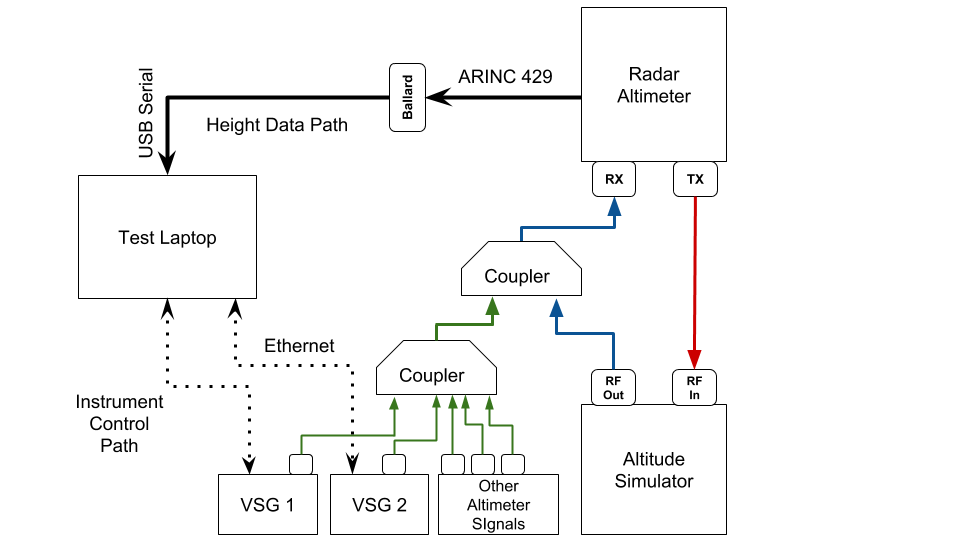
\includegraphics[scale=.5]{Wideband_Test_Setup.png}
\caption{Expanded Test Bench For Wideband and Altimeter Interference.}

\label{fig:Wideband}

\end{figure}
\subsection{Adding The Second VSG}
Early testing clearly demonstrated the effects of interference bandwidth on the altimeter signal processing. Wider bandwidth OFDM signals caused the altimeter to break at a lower RF Carrier power than narrower bandwidth signals. This dependence made it necessary to demonstrate the effects of OFDM filling the entire 4200 to 4400 MHz band. (See Section~\ref{} Results of initial testing) However, the Rhode and Schwarz SMU 200A VSG used for initial testing could only support an 100 MHz OFDM signal due to bandwidth limitations on the instrument.  

To supplement, this a Rhode and Schwarz SMW 200A was located in the senior design lab, and was appropriated (with permission of the owner) for the purpose of expanding the testing capability. This slightly newer VSG could support a 160 MHz OFDM signal, and when used in conjunction with the first VSG, the two filled the full spectrum. A secondary goal of this process is to test the effects of proposed Cellular networks in adjacent bands to the altimeter band while still maintaining simulated WAIC Interference. The dual VSG setup allowed for the one VSG to simulate in band interference while the other swept through out of band signals. 

\subsubsection{Providing Isolation to the VSGs}
\begin{figure}[ht]
\centering
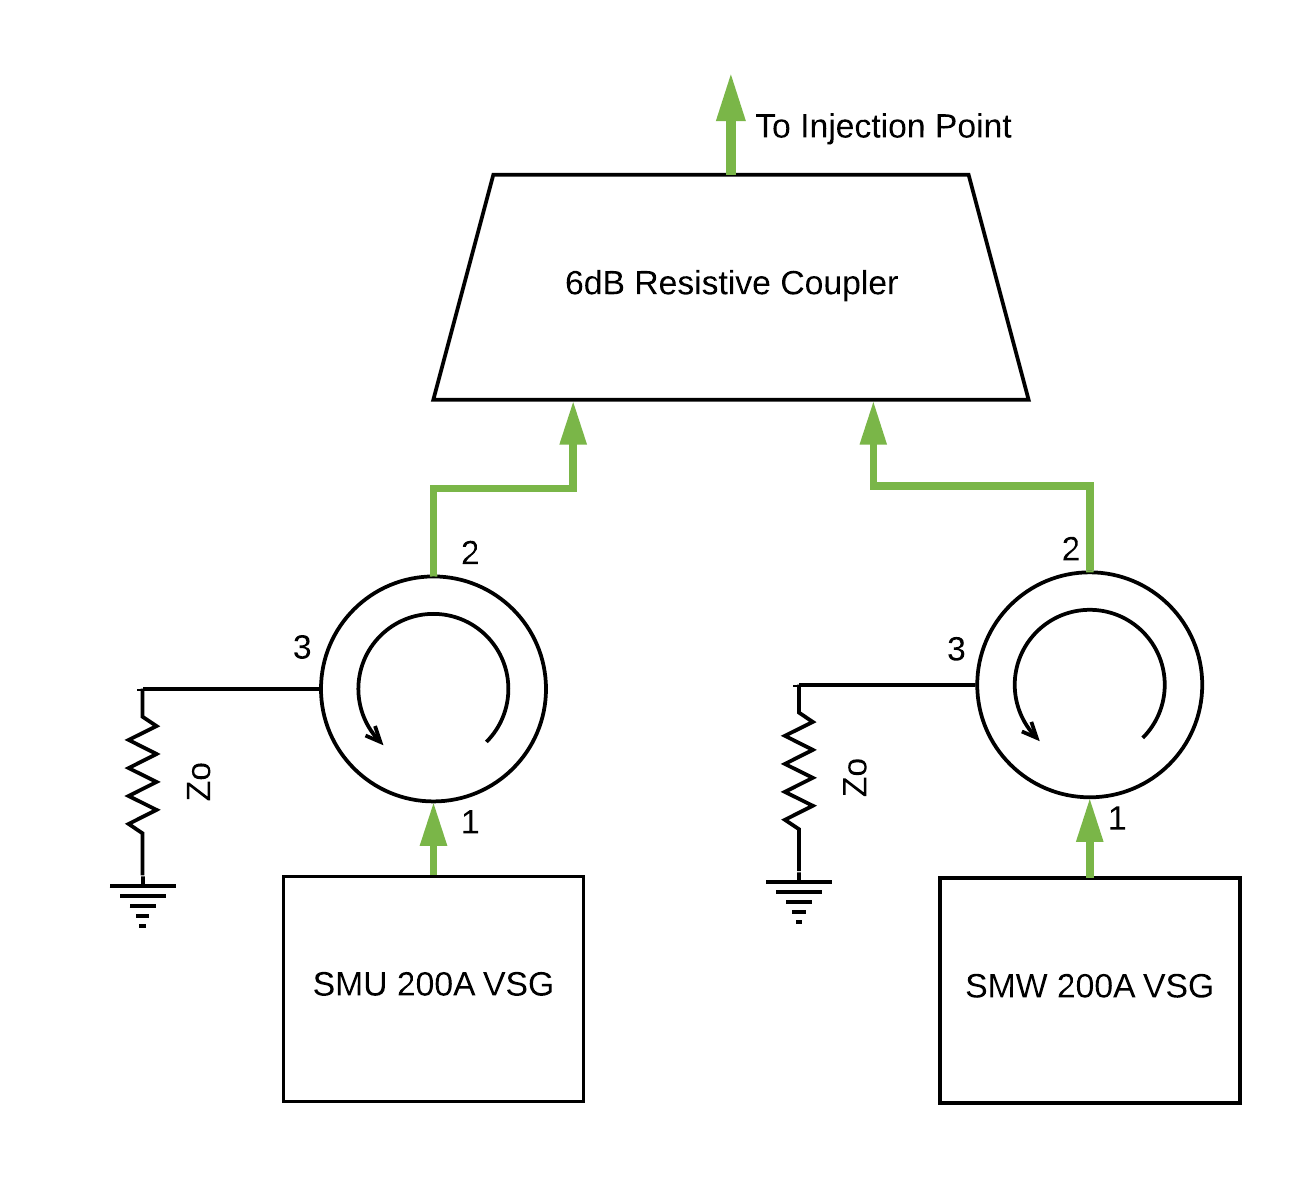
\includegraphics[scale=1]{Isolators_Coupler.PNG}
\caption{Circulator with Matched Load Added to Protect VSGs}

\label{fig:circulator}
\end{figure}
One problem with using the 6dB resistive power divider to couple the interference from the two VSGs together was the lack of isolation. The coupler provides no directionality, and signals which enter one port are split equally between the two other ports. This was hazardous since the high interference powers being tested could damage the other VSG if fed into the \textit{RF Out} port in reverse. 

AVSI began looking into purchasing other couplers to provide higher isolation to the VSGs, when the Garmin engineer participating in the project offered to contribute two circulators which could function as isolators. By placing a matched load at port 3, most power entering from port 2 is absorbed into the load, with very little (ideally none) reflected back to port 2 or allowed to pass to port 1. Signals entering port 1 experience a small attenuation due to the properties of the circulator. Figure ~\ref{fig:circulator} shows how circulators in this configuration provide isolation to the VSGs when coupled together. 

\subsubsection{Achieving Higher Power Interference}

\begin{figure}[ht]
\centering
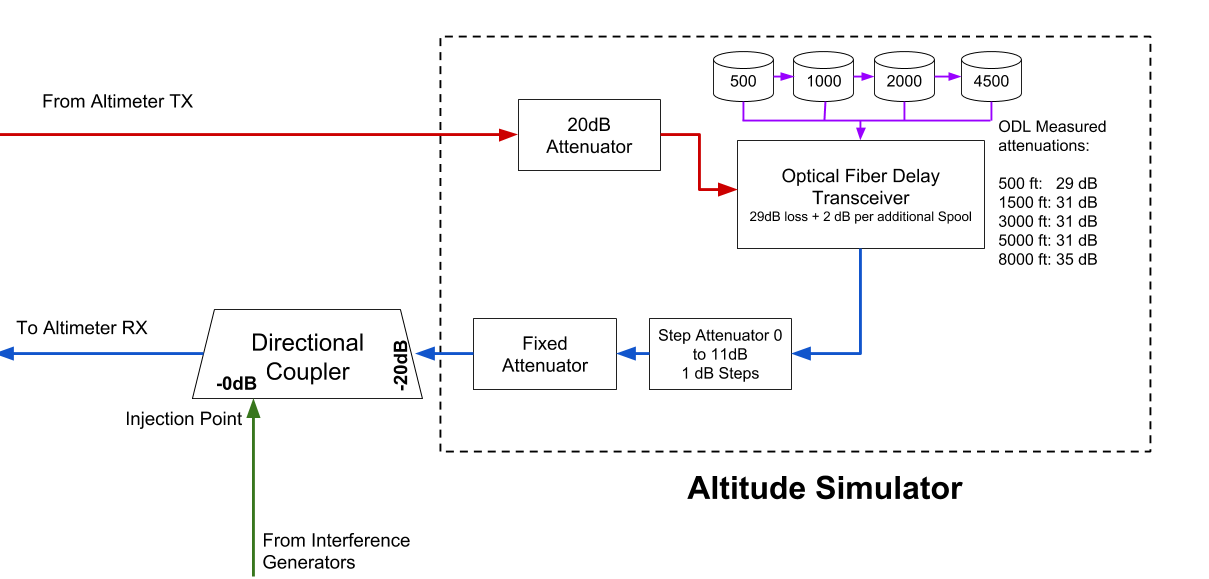
\includegraphics[scale=.4]{Coupler_Swap.png}
\caption{Modifications for Higher Interference Power}

\label{fig:coupler_swap}

\end{figure}


While the isolators protected the VSGs from damaging one another, they also added more attenuation into the line, meaning the altimeter RX received a lower RF Power than in earlier tests. This upper limit, caused by the Peak Envelope Power (PEP) limitation of the VSGs, prevented tests from locating the breaking point of an altimeter sometimes. 


The setup was modified again to fix this. The 20dB attenuator placed on the output of the optical delay line in the altitude simulator was removed, and the 16dB directional coupler was replaced with a 20 dB directional coupler. Figure~\ref{fig:coupler_swap} shows how the output of the altitude simulator fed into the 20dB loss port of the directional coupler to compensate for removing the fixed attenuator, and the interference injection point was moved to a port with (ideally) no attenuation. Additionally, this configuration was advantageous because the step attenuator and variable fixed attenuator settings for different altitudes did not have to be recalculated. 

A Vector Network Analyzer S21 measurement was taken to verify the isolation provided by this configuration, as well as the attenuation between each VSG RF port and the altimeter RX. 

\subsection{Simulating Altimeter Interference}
The other major modification shown in Figure~\ref{fig:Wideband} was the addition of other altimeter signals to the interference already being tested. This addition intended to move the setup closer to the real-life worst case scenario for the interference an altimeter might be subjected to. The test bed was configured to replicate an approach for landing scenario used in earlier compatability investigations. A series of VCOs were calibrated and driven by function generators to generate the external altimeter signals, and programmable and fixed attenuators configured the distance of each altimeter signal from the receiver. The VSG setup was configured to simulate the interference of the full 4.2 to 4.4 GHz band filled with WAIC signals from other aircraft, with a goal of determining what WAIC radiated power limitations were necessary to protect altimeters. Finally, all of these signals were coupled together with the VSG signals to send toward the interference injection point. 


\subsubsection{Determining the Worst-Case Scenario Geometry}
A worst-case scenario for the interference experienced by a victim altimeter from other aircraft was developed in the 2014 compatibility studies submitted to the ITU~\cite{noauthor_compatibility_2014}. The authors determined that the altimeter data was most important to the safety of a flight during the landing phase of operation. When aircraft line up for approach, they typically maintain a distance of around 5 km, which makes interfernce from WAIC signals or other altimeters aboard these neighbors negligible. On the other hand, aircraft taxiing or in holding adjacent to a runway can achieve distances less than 300 m to the victim RA. These aircraft could present a significant hazard to nearby altimeter receivers if WAIC power limitations are not developed in the context of this scenario. 

\begin{figure}[ht]
\centering
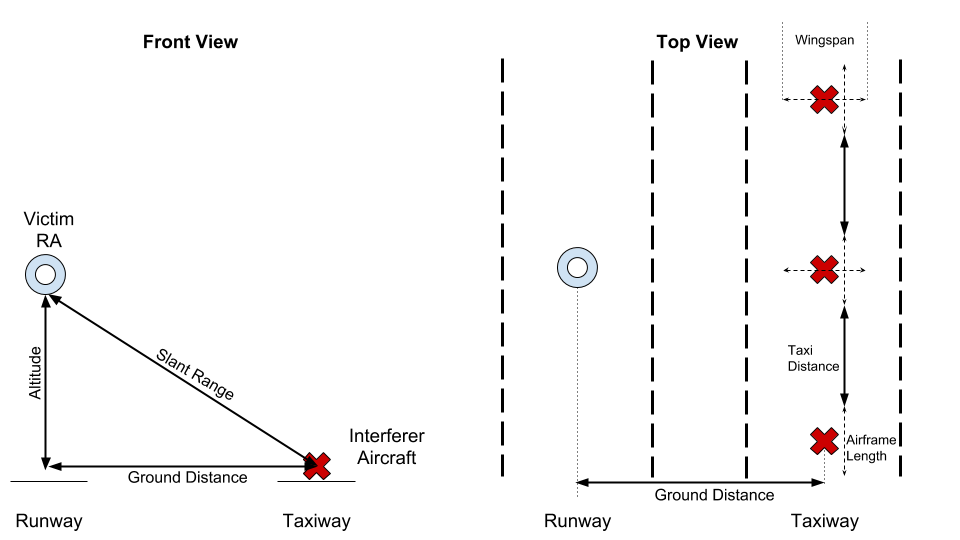
\includegraphics[scale=.5]{Victim_RA.png}
\caption{Geometry Used in ~\cite{noauthor_compatibility_2014} for Interference During Landing Scenario}

\label{fig:victim_ra}

\end{figure}

Figure~\ref{fig:victim_ra} shows the geometry from~\cite{noauthor_compatibility_2014} which was also used for the this compatibility study. The markers represent the center of the airframe for each aircraft. Three parameters specify the distance of aircraft to one another in this scenario. The \textit{ground distance} between the runway and adjacent taxiway, the \textit{altitude} of the victim aircraft during descent, and the \textit{taxi distance} from nose to tail of aircraft in the queue for takeoff. A \textit{slant range} between the victim RA and an interferer can be determined using these parameters. Additionally, the \textit{wingspan} and \textit{airframe length} of each plane plays a role in the location of potential interferers.

The path losses from simulated WAIC signals were calculated in the context of this geometry. Altimeter transmitters and receivers were located at the center of the airframe, directly underneath each aircraft. Interferers modeling WAIC devices for applications internal to the aircraft were grouped together at the center-point inside of each airframe. For applications external to the aircraft, Interferers were grouped together at the wing tip closest to the victim altimeter. This model provides a worst case scenario for WAIC interference, because in reality WAIC devices would be distributed throughout an airframe according to the need of an application, rather than grouped together at the point closest to an external aircraft's receiver. 
%	
%	Initially, the authors attempted to model all WAIC devices as omnidirectional point sources (OPS's)~\cite{noauthor_compatibility_2014}. This model is simple yet provides a relatively accurate accounting for the pattern given off by antennas at large distances. However, the OPS model assumed homogeneous radiation in every direction. The authors found that external WAIC devices violated the protection criteria for incumbant services in the band. To mitigate this, a radiation pattern was applied which limited power in critical directions. 

%	While the aforementioned study focused primarily on WAIC interference, 
In addition to specifying the path loss experienced by WAIC interferers located at a minimum slant range, this geometry also served to model the interference subjected to the victim RA by other altimeters. While most altimeters are designed to handle external altimeter signals, the \textit{combination} of these signals with WAIC interference leads to more stress on the victim receiver. This geometry models the locations of external altimeters along with WAIC signals to simulate this effect. Path losses assigned to each simulated altimeter are specified by the location in this geometry. 

\begin{figure}[ht]
\centering
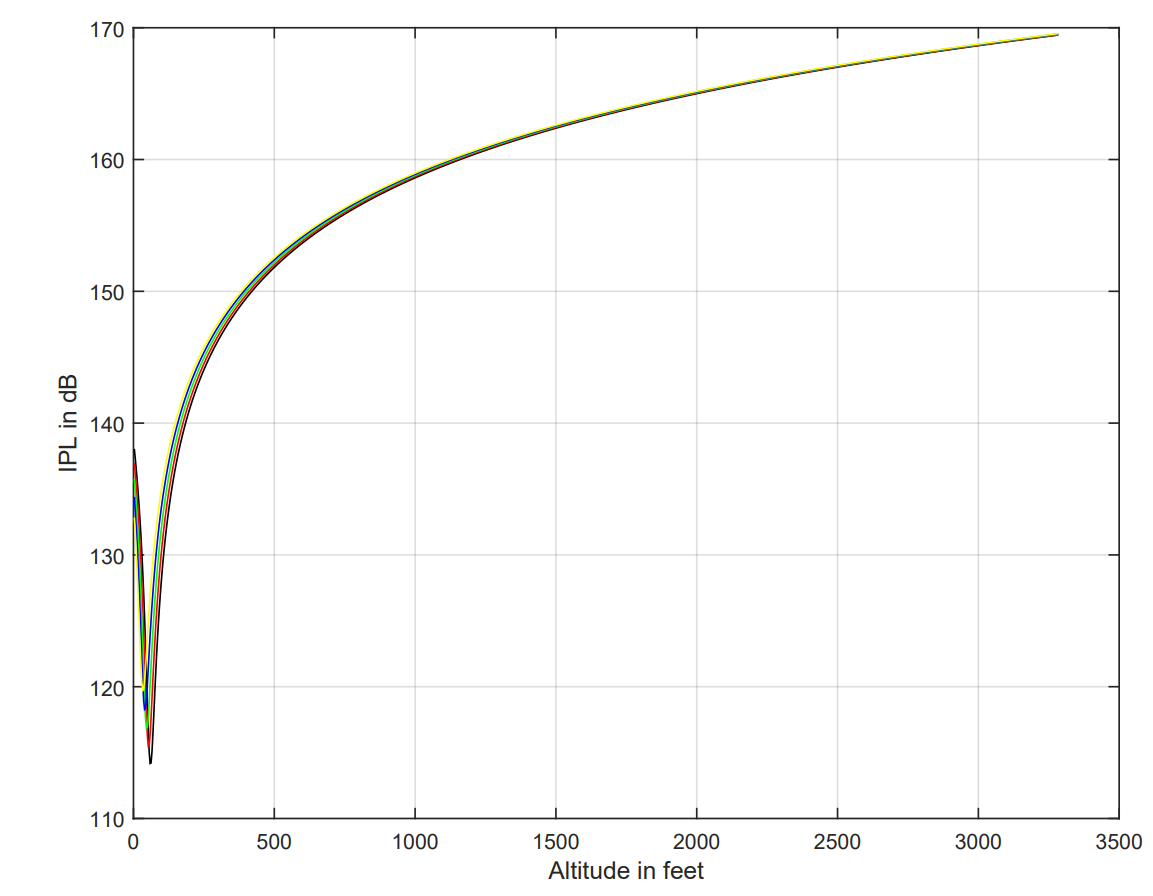
\includegraphics[scale=.6]{IPL_Plot.png}
\caption{Plot of IPL values for 15 closest aircraft}

\label{fig:IPL}

\end{figure}

The geometry was then modeled in a Matlab script by Airbus as a contribution to this project. The victim aircraft approached for  a landing on a 3 degree glide slope, and the interference path loss (IPL) from each aircraft on adjacent taxiways were modeled  in the script. Figure~\ref{fig:IPL} shows the results of this analysis. The IPL value for each of the 15 nearest aircraft are shown as a function of height, with a minimum occurring at approximately 200ft due to the angle of of reflected interference signals offering the shortest direct path into the victim RX antenna. From this, the committee drew the conclusion that the worst case altitude for this geometry occurred at approximately 200ft. 

However, the lab test equipment had available test altitudes of only 40 and 500ft. After some deliberation, the 500ft altitude was chosen for the approach tests. By configuring the IPLs for the 200 ft case, and the altimeter loop loss for a 500ft case, the signal to interference ratio went from the real life worst case scenario to a so-called `super' worst case scenario: $$\frac{S(200ft)}{I(200ft)}\leq\frac{S(500ft)}{I(200ft)}$$
This super worst case would be used to configure interfering altimeters for the landing simulation.


\subsubsection{Simulating Individual Altimeter Signals}
Several approaches were considered to simulate altimeter signals for the approach scenario. While software defined radios were appealing for the convenience the offered in modifying the test bed, they were in the end rejected in favor of a series of Voltage Controlled Oscillators (VCOs) controlled by function generators. The major advantage seen in the VCO approach was the simplicity of explaining the test scenario to regulators, as opposed to having to present another piece of software.

Eight two channel function generators and 16 VCOs were ordered for this purpose. The function generators were configured to output a triangle voltage wave to drive the VCOs in the FMCW pattern seen in Figure~\ref{fig:FMCW}. The min and max voltage on the triangle wave correspond to the VCO setting for the min and max frequency of the simulated altimeter waveform. The frequency of the voltage waveforms was varied between different VCOs to simulate the varying pulse frequencies exhibited by different altimeters as well as to provide randomness to the simulation. It was considered critical that the different simulated altimeter signals were asynchronous to provide a realistic scenario. 


\subsubsection{Connecting the VCO Signals}
Figure~\ref{fig:VCO_Coupler} shows how the VCO signals were coupled together to simulate 16 different altimeter signals. While the initial plan had been to simulate every altimeter on the 15 closest aircraft to the victim, the VCOs became backordered after the first 16, and empirical studies showed that the effects of the higher power ``on board'' simulated altimeter signals overwhelmingly dominated the effects of the ``external'' VCOs. 
\begin{figure}[ht]
\centering
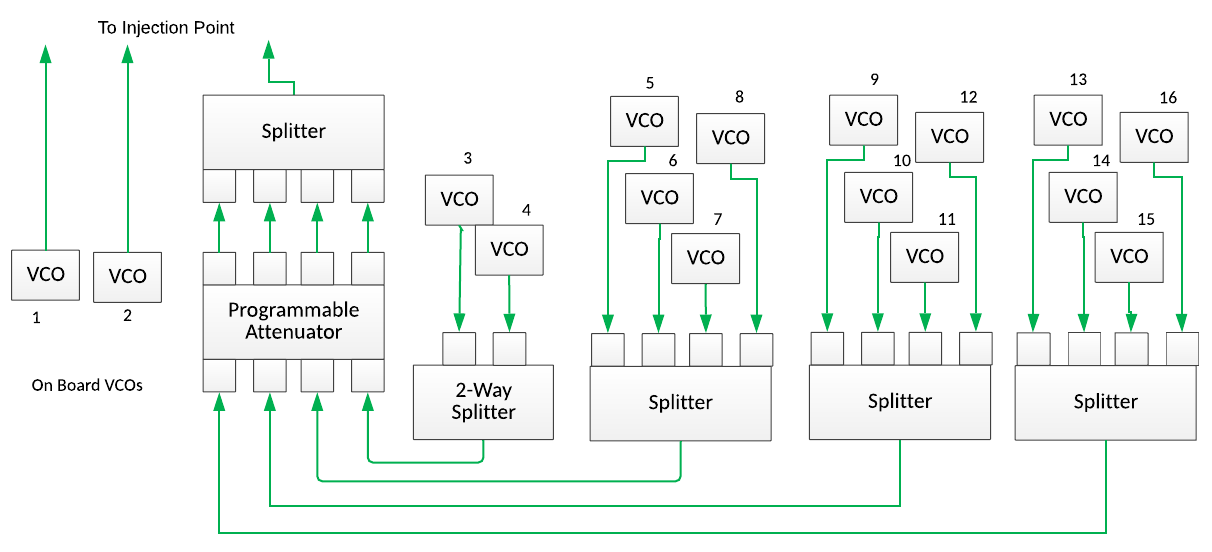
\includegraphics[scale=.85]{Altimeter_Signal_Simulator.png}
\caption{Diagram of Combined 16 Simulated ALtimeter Signals}

\label{fig:VCO_Coupler}

\end{figure}
Each VCO was configured to simulate the RF power of an altimeter (typically 30dBm), and the associated path loss from interferer TX to victim RX. This was accomplished with a variety of sources of attenuation. Each VCO output 4dBm of RF power according to the data-sheet. Fixed attennuators could be placed at the RF output of each VCO to achieve individualized IPL values. Each splitter contributed 6dB of attenuation to a connected path. The 4-channel programmable attenuator offered programmable values between 0 and 63 dB of attenuation. Lab measurements found that the programmable attenuator contributed 4 dB with a programmed setting of 0 and confirmed that each dB of programmed attenuation added a dB to this value. Finally, the attenuation from the interference injection point to the altimeter RX is added to the path loss. 

\begin{table}[]
\begin{tabular}{c||ccccc}
\textbf{VCO} & Power {[}dBm{]} & Fixed {[}dB{]} & Programmable {[}dB{]} & Path Loss {[}dB{]} & Power at RX {[}dBm\} \\ \hline
\textbf{1}   & 4               & -18              & X                     & -16                & -30                  \\
\textbf{2}   & 4               & -18              & X                     & -16                & -30                  \\ \hline


\textbf{3}   & 4               & 0              & -56                   & -40                & -92                  \\
\textbf{4}   & 4               & 0              & -56                   & -40                & -92                   \\ \hline


\textbf{5}   & 4               & 0              & -26                    & -40                & -62                 \\
\textbf{6}   & 4               & 0              & -26                    & -40 			& -62                  \\
\textbf{7}   & 4               & 0              & -26                    & -40                & -62                  \\
\textbf{8}   & 4               & 0             & -26                    & -40                & -62                  \\ \hline


\textbf{9}   & 4               & 0              & -26                   & -40                & -62                  \\
\textbf{10}  & 4               & 0              & -26                   & -40                & -62                  \\
\textbf{11}  & 4               & -23            & -26                   & -40               & -85                  \\
\textbf{12}  & 4               & -23             & -26                   & -40                & -85                  \\ \hline


\textbf{13}  & 4               & 0              & -49                   & -40                & -85                  \\
\textbf{14}  & 4               & 0              & -49                   & -40                & -85                  \\
\textbf{15}  & 4               & 0              & -49                   & -40                & -85                  \\
\textbf{16}  & 4               & 0              & -49                   & -40                & -85                 
\end{tabular}
\caption{VCO Attenuation Configurations for 200ft Worst Case}
\label{tab:VCO_Pow}
\end{table}
\subsubsection{Calibrating The VCOs}
The VCOs ordered for this purpose could go beyond the 4.2-4.4 GHz range, but a control voltage did not necessarily map to the same frequency across different VCOs. This meant that each of the 16 VCOs needed to be calibrated. First, each VCO was connected to a 5V power supply, and the control pin was connected to a separate power supply. The RF output of each VCO was connected to the spectrum analyzer for observation. The frequency output by a VCO under constant voltage had a bit of a `wobble' to it, so the spectrum analyzer was configured to display a \textit{Max Hold} instead of a real time measurement. After a VCO was left on a control voltage for several seconds, a marker was used to locate the frequency of the maximum output at that setting. 

The first calibration sweep went from 0 to 5 V in 1 V increments.  The goal of this broad sweep was to get an approximation for where the 4.2 and 4.4 GHz voltages were for each VCO. The VCO output was observed on the spectrum analyzer to determine the operating frequency at that control voltage. The search found that a majority of the 4.2-4.4 GHz band lied in the 2-5V range for these VCOs. The initial sweep was not fine enough to capture the desired minimum and maximum frequencies for each VCO. 


% Please add the following required packages to your document preamble:
% \usepackage{booktabs}
\begin{table}[]
\centering
\begin{tabular}{@{}c|cc|cc|ccc@{}}
    & \multicolumn{2}{c|}{Lower} & \multicolumn{2}{c|}{Upper} & \multicolumn{3}{c}{\textbf{Function Generator Setting}}       \\
VCO & Voltage  & Freq {[}GHz{]}  & Voltage  & Freq {[}GHz{]}  & \textbf{Center} & \textbf{Amplitude} & \textbf{Freq {[}Hz{]}} \\ \midrule
1   & 2.2      & 4.237           & 4.0      & 4.362           & 3.1             & 1.8                & 143                    \\
2   & 1.6      & 4.236           & 3.5      & 4.367           & 2.6             & 1.9                & 143                    \\
3   & 2.2      & 4.232           & 4.1      & 4.365           & 3.2             & 1.9                & 143                    \\
4   & 2.0       & 4.233           & 3.9      & 4.364           & 3.0             & 1.9                & 111                    \\ \midrule
5   & 1.8      & 4.233           & 3.7      & 4.364           & 2.8             & 1.9                & 133                    \\
6   & 2.0      & 4.238           & 3.8      & 4.362           & 2.9             & 1.8                & 133                    \\
7   & 1.8      & 4.233           & 3.7      & 4.365           & 2.8             & 1.9                & 133                    \\
8   & 1.7      & 4.233           & 3.6      & 4.368           & 2.7             & 1.9                & 118                    \\ \midrule
9   & 2.0      & 4.235           & 3.9      & 4.367           & 3.0             & 1.9                & 118                    \\
10  & 2.0      & 4.233           & 3.9      & 4.365           & 3.0             & 1.9                & 118                    \\
11  & 2.0      & 4.238           & 3.8      & 4.362           & 2.9             & 1.8                & 111                    \\
12  & 2.1      & 4.236           & 3.8      & 4.366           & 3.0             & 1.7                & 129                    \\ \midrule
13  & 1.8      & 4.235           & 3.7      & 4.364           & 2.8             & 1.9                & 129                    \\
14  & 2.0      & 4.235           & 3.7      & 4.366           & 2.9             & 1.7                & 129                    \\
15  & 2.1      & 4.237           & 3.8      & 4.368           & 3.0             & 1.7                & 143                    \\
16  & 2.3      & 4.233           & 4.2      & 4.365           & 3.3             & 1.9                & 143                   
\end{tabular}
\caption{VCO Calibration Results and Corresponding Function Generator Settings}
\label{tab:VCO_Cal}
\end{table}


A second calibration was attempted to fix this. The goal was to get the simulated FMCW waveforms centered at 4.3 GHz, with a span of $\pm65$ MHz. Using 100 mV increments, the previous calibration procedure was repeated, this time explicitly searching for the control voltages corresponding to the frequencies closest to 4235 MHz and 4365 MHz. These were achieved with a $\pm3$ MHz precision. The 100 mV increments from the calibration process were chosen due to the precision available to the function generators. It was this limitation that lead to the 3 MHz frequency precision. The full calibration results are shown in Table~\ref{tab:VCO_Cal}.

Once the lower and upper voltages were determined, a simple calculation found the center voltage and amplitude necessary to feed into the function generators. In addition to the amplitude and offset settings available to the function generator, the control voltage wave had a frequency parameter. These were chosen in part with enough variance so that there was no synchronization between the different simulated altimeter signals. Random crossover of the simulated altimeter signals was desired to closely match the real world interference scenario. Function generator parameters are also shown in Table~\ref{tab:VCO_Cal}.

\subsubsection{VCO Protection Circuit}
While the VCO's were designed to operate with a control voltage between 0 and 5V, they were later verified to tolerate a maximum 6.5V signal before a catastrophic failure. Because the Function Generators were capable of up to a 20V peak to peak signal, they could damage a VCO with an accidental twist of a knob, and a protection circuit was needed.

\begin{figure}[ht]
\centering
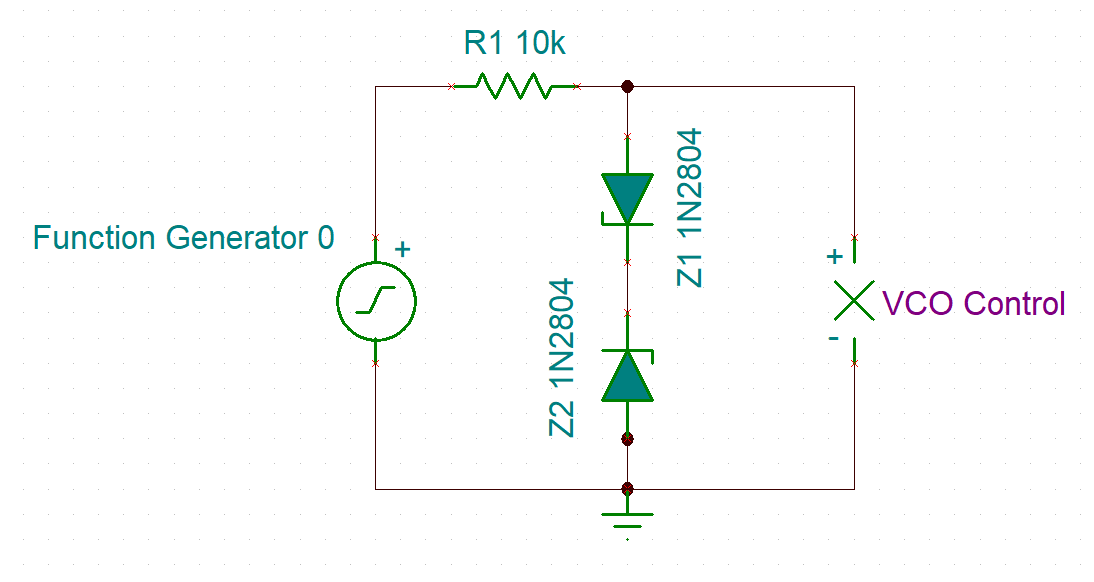
\includegraphics[scale=.6]{Protective_Circuit.png}
\caption{Double Clipper Protective Circuit}

\label{fig:Clipper}

\end{figure}


 Initially, the protective circuit seemed even more urgent. The voltage setting on the function generator starts at 10V upon power up, but does not clearly mark whether this is a peak to peak voltage or $\pm10$ V. Compounding this ambiguity, when the output of the function generators was measured with an oscilloscope, the multiplier setting was set to 2X. This made it appear to be a $\pm10$ V signal on startup which would fry the VCO if the function generator was accidentally power cycled. This error was only noticed after the protective circuit was designed and built. 

After some searching, a limiter or `clipper' circuit was decided on to protect the VCOs. Clippers consist of a resistor and one or two diodes. Various designs of clipper circuits and the trade-offs between them are discussed in~\cite{sedra_microelectronic_2015}. Based on this discussion, a double clipper like the one shown in Figure~\ref{fig:Clipper} was decided on. Two zener diodes begin to limit the upper and lower voltage extremes once they pass the diode's cutoff voltage. A resistor is placed in series with the diodes to limit the current in the diodes to safe levels. 
\begin{figure}[ht]
\centering
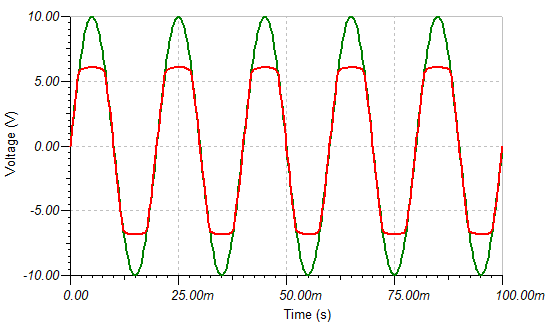
\includegraphics[scale=1.3]{Clipped_Sin_Wave.png}
\caption{Double Clipper Protective Circuit}

\label{fig:Clipped_Sin}

\end{figure}

The clipper circuit was modeled in a spice program so that different diode cutoff voltages could be tried. Simulations showed that the output voltage from this circuit would typically go slightly above the cutoff voltage. Because of this, a Zener diode with a 6 Volt cutoff was chosen to limit the output below the 6.5 Volt failure point. A simulated ouptut from the clipper circuit waveform is shown in Figure~\ref{fig:Clipped_Sin}. A $\pm$10 V sin wave is fed from the function generator, shown in green, and the `clipped' waveform is shown in red. The circuit allows voltages close to the failure point without reaching it. This performance was verified with an oscilloscope for each function generator output.


\subsection{Testing Lower Altitudes}
A final major modification from the initial test regimen involved adding different altitude simulator configurations to the rotation to achieve lower altitudes. These were touched on briefly in Section~\ref{sub:Implementing}. Lower altitude tests were first started before the approach scenario analysis determined that 200ft was the worst case scenario. Once the worst case analysis was determined, lower altitude tests were continued to provide supplementary evidence at another altitude in the landing scenario. 
\begin{figure}[ht]
\centering
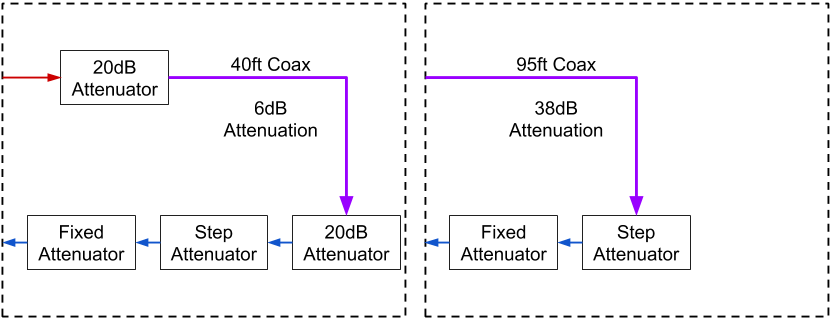
\includegraphics[scale=.55]{Low_Altitude_Simulator.png}
\caption{Left: 40ft Altitude Simulator; Right: 95 ft Altitude Simulator}

\label{fig:Low_Altitudes}

\end{figure}

Two different coaxial cables were used to simulate different altutudes below the 500ft threshold the optical delay line was capable of. Firstly, a coaxial cable providing 40ft altitude was located in the lab for this purpose, shown on the left of Figure~\ref{fig:Low_Altitudes}. When measured with a VNA, this coax had only a 6dB attenuation, so two 20dB fixed attenuators were placed on either side to increase the attenuation. This allowed the same step and fixed attenuator combination from Figure~\ref{fig:Altitude_Simulator} to easily achieve the DO-155 attenuation from Table~\ref{tab:loop loss}. The 40ft altitude simulator underwent the same modification as the Fiber Optic Line in Figure~\ref{fig:coupler_swap}, which allowed higher power interference signals without modifying the fixed and step attenuator settings in use. 

The second altitude simulator used during these tests was a 95ft cable which was ordered after a significant nubmer of 40ft tests had been run. The 40ft tests had revealed a problem where one of the newer altimeters (with more advanced signal processing) would not output an altitude below a certain threshold unless it detected that the aircraft was moving. This precipitated the 95ft tests so that an altitude below the 200ft worst case could be tested across all units. The 95ft cable was a lower quality coax than the 40ft cable, and when measured with a network analyzer showed an approximately 38dB attenuation at 4.3 GHz. This was confirmed to be approximately the expected attenuation for this length of coax from the manufacturer's website. Once again, a fixed and step attenuator allowed the altitude simulator to be fully adjustable and achieve the DO-155 specified attenuation. 

%%%%%%%%%%%%%%%%%%%%%%%%%%%%%%%%%%%%%%%%%%%%%%%%%%%%%%%%%
\section{Expanded Setup Test Plans}
The different modifications discussed above were combined into a full setup. This was used to test the altimeters in approach scenarios, to detremine a breaking point for full spectrum interference for the purposes of regulation, and to investigate the effects of adjacent band interference signals.
\subsection{Full Setup Diagram}
\begin{figure}[ht]
\centering
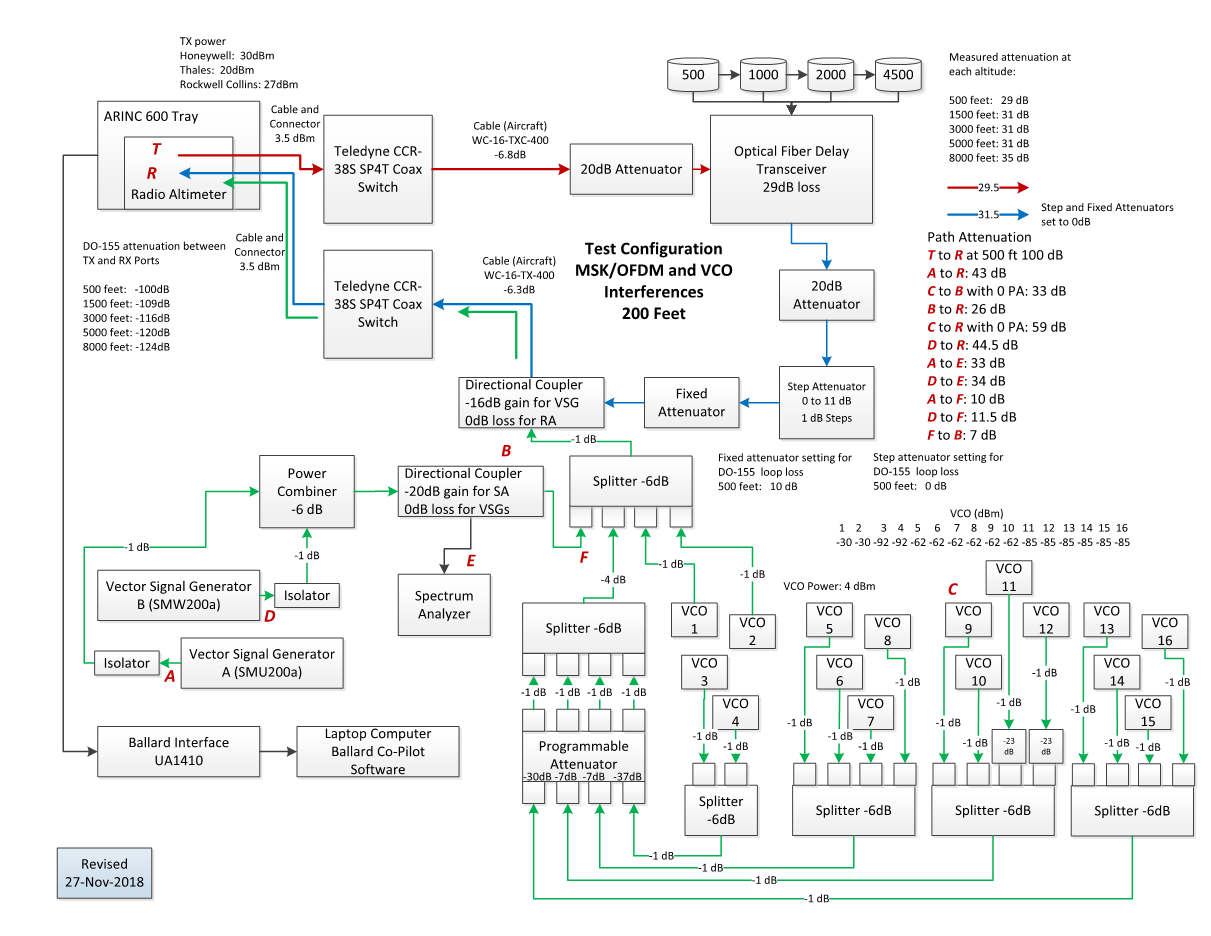
\includegraphics[scale=.75]{Full_Setup.PNG}
\caption{Full test setup combining various modifications to Figure~
\ref{fig:Initial}}

\label{fig:combined}

\end{figure}
Figure~\ref{fig:combined} shows the full test setup diagram. The modifications covered in Section~\ref{sec:expanding}, including the second VSG, isolators to protect the VSG's, and the VCO setup to simulate 16 other altimeter signals are included in this diagram. Depending on the desired test scenario, the lower altitude simulators from Figure~\ref{fig:Low_Altitudes} were substitute in for the optical delay line, and as tests progressed, the modification shown in Figure~\ref{fig:coupler_swap} allowed for higher interference powers. 

\subsection{Breaking Point Definition}\label{sub:break}
Early tests showed that powerful itnerference signals would not only cause outliers which broke the ARINC 707~\cite{noauthor_arinc_2009} standards, but also caused a distortion of the mean height. Since presenting a more restrictive standard to regulators was seen as beneficial, a stronger definition of breaking point was introduced compared to previous tests. Thus, the breaking point definition was expanded to include either a) a maximum height error beyond the 2\% or 1.5 feet allowable by ARINC 707, b) any height reading labeled NCD, or \textbf{c)} a mean height error greater than 0.5\%. 

\subsection{In Band Testing}\label{sub:ib}
\begin{table}[]
\begin{tabular}{c|c|c|c|c|c|c|c}
\multicolumn{3}{c|}{\textbf{Interference Signal}} & \multicolumn{3}{c|}{\textbf{VSG RF Power}} & \multicolumn{2}{c}{\textbf{Power Durations}} \\
Modulation    & Bandwidth   & Center     & Min         & Step    & Max       & ON                & OFF              \\ \hline
OFDM          & 200 MHz     & 4300 MHz   & -56 dBm     & 2 dB    & 19 dBm    & 60 s              & 20 s            
\end{tabular}
\caption{Interference Signals for Wideband Testing}
\label{tab:Wideband}
\end{table}


Table~\ref{tab:Wideband} shows the interference signals used to run the in band dual vsg tests. The purpose of these tests was to find the `breaking point' of each altimeter when subjected to a full band of interference signals under worse than possible real life conditions. When the worst breaking point among the altimeters sampled was found, the comittee would add a margin of a few dB and propose that number to regulators. These results are discussed in Section~\ref{sec:dvsg_ib_results}
\subsection{Out of Band Testing}\label{sub:oob}
Finally, Table~\ref{tab:oob} shows a representative test definition for the out of band tests run under AFE76s2. These tests were designed to develop an RF power mask on the upper and lower side of the radio altimeter bands. This mask could be brought to regulators with a proposal to limit users in adjacent bands a certain margin below the altimeter breaking point. 

Initially, the 5MHz wide OFDM signals used in previous tests were tried. However, after initial results came in, more granular sweep was desired, so the bandwidth was reduced to the 200kHz signals shown in Table~\ref{tab:oob}. When the 200kHz waveform was measured on the spectrum analyzer, it was noticed that the waveform center was slightly offset from the carrier frequency. The lower edge of the waveform was approximately 35 kHz below the carrier, and the upper edge was approximately 165 kHz above the carrier. 

Since the test goal was to step an OFDM waveform with the upper edge directly on 4.2 GHz, and step away from the altimeter band till the upper edge was 5 MHz away from the band edge. Waveforms in the upper adjacent band were placed at 4200.035 MHz and stepped to 4205.035 MHz for the same reason.

These tests are ongoing at the time of writing, and will likely go through a few more iterations before being finalized, but preliminary results from this test definition are discussed in Section~\ref{sec:dvsg_oob_results}

\begin{table}[]
\begin{tabular}{cc|cc|ccc|cc}
\multicolumn{4}{c|}{\textbf{Interference Signal}}                                     & \multicolumn{3}{c|}{\textbf{VSG RF Power}} & \multicolumn{2}{c}{\textbf{Durations}} \\
                                &           & \multicolumn{2}{c|}{Center Frequencies} &                &            &              &                               &         \\
\multicolumn{1}{c|}{Modulation} & Bandwidth & Min {[}MHz{]}      & Max {[}MHz{]}      & Min            & Step       & Max          & \multicolumn{1}{c|}{ON}       & OFF     \\ \hline
\multicolumn{1}{c|}{OFDM}       & 200 kHz   & 4194.835           & 4199.835           & -60 dBm        & 2 dB       & 10 dBm       & \multicolumn{1}{c|}{10 s}     & 10 s    \\
\multicolumn{1}{c|}{OFDM}       & 200 kHz   & 4194.835           & 4199.835           & -60 dBm        & 2 dB       & 10 dBm       & \multicolumn{1}{c|}{10 s}     & 10 s   
\end{tabular}
\caption{Interference Signals For Out Of Band Testing}
\label{tab:oob}
\end{table}

%%%%%%%%%%%%%%%%%%%%%%%%%%%%%%%%%%%%%%%%%%%%%%%%%%%
%
%  New template code for TAMU Theses and Dissertations starting Fall 2016.  
%
%
%  Author: Sean Zachary Roberson
%  Version 3.17.09
%  Last Updated: 9/21/2017
%
%%%%%%%%%%%%%%%%%%%%%%%%%%%%%%%%%%%%%%%%%%%%%%%%%%%
%%%%%%%%%%%%%%%%%%%%%%%%%%%%%%%%%%%%%%%%%%%%%%%%%%%%%%%%%%%%%%%%%%%%%%
%%                           SECTION III
%%%%%%%%%%%%%%%%%%%%%%%%%%%%%%%%%%%%%%%%%%%%%%%%%%%%%%%%%%%%%%%%%%%%%

\chapter{RESULTS}
The radio altimeter tests described in this work were developed over a two year long process which can be approximately separated into three distinct phases of testing. The initial testing results discussed in Section~\ref{sec:initial_results} characterized the basic response of altimeters to various types of interference. These led to another set of tests aimed at more systematically demonstrating altimeter performance under more conservative than real life conditions. The in-band testing in Section~\ref{sec:dvsg_ib_results} demonstrated what power level of a full 200~MHz of WAIC interferers would break an altimeter in the worst case scenario. Finally, the Out of Band testing regimen investigated altimeter performance when subjected to cellular interference in neighboring bands. Preliminary out of band results are discussed in Section~\ref{sec:dvsg_oob_results}. Results of the two later testing regimens were used to propose maximum radiated power values to  regulators, as well as in continuing discussions. 

\section{General Plotting Scripts}
This setup introduces the two general types of plots used across all tests, called `Height Plots' and `Stat Plots' respectively. The form of these was evolved over the course of different testing regimens to communicate the results from each effectively, but the basic plots introduce a standard format in which results from an altimeter test are displayed. 


\subsection{Height Plots}
The first attempts at a representation of data taken during these tests developed into \textit{height plots}. The goal of the height plot is to provide a visualization of how the interference signals from the VSG  distort the altitude signal output by an altimeter over time. In each altimeter test, a height plot is generated for each unique combination of center frequency and modulation format under test. Figure~\ref{fig:height_plot_example} shows an height plot from the initial testing regimen. 

\begin{figure}[h!]
	\centering
	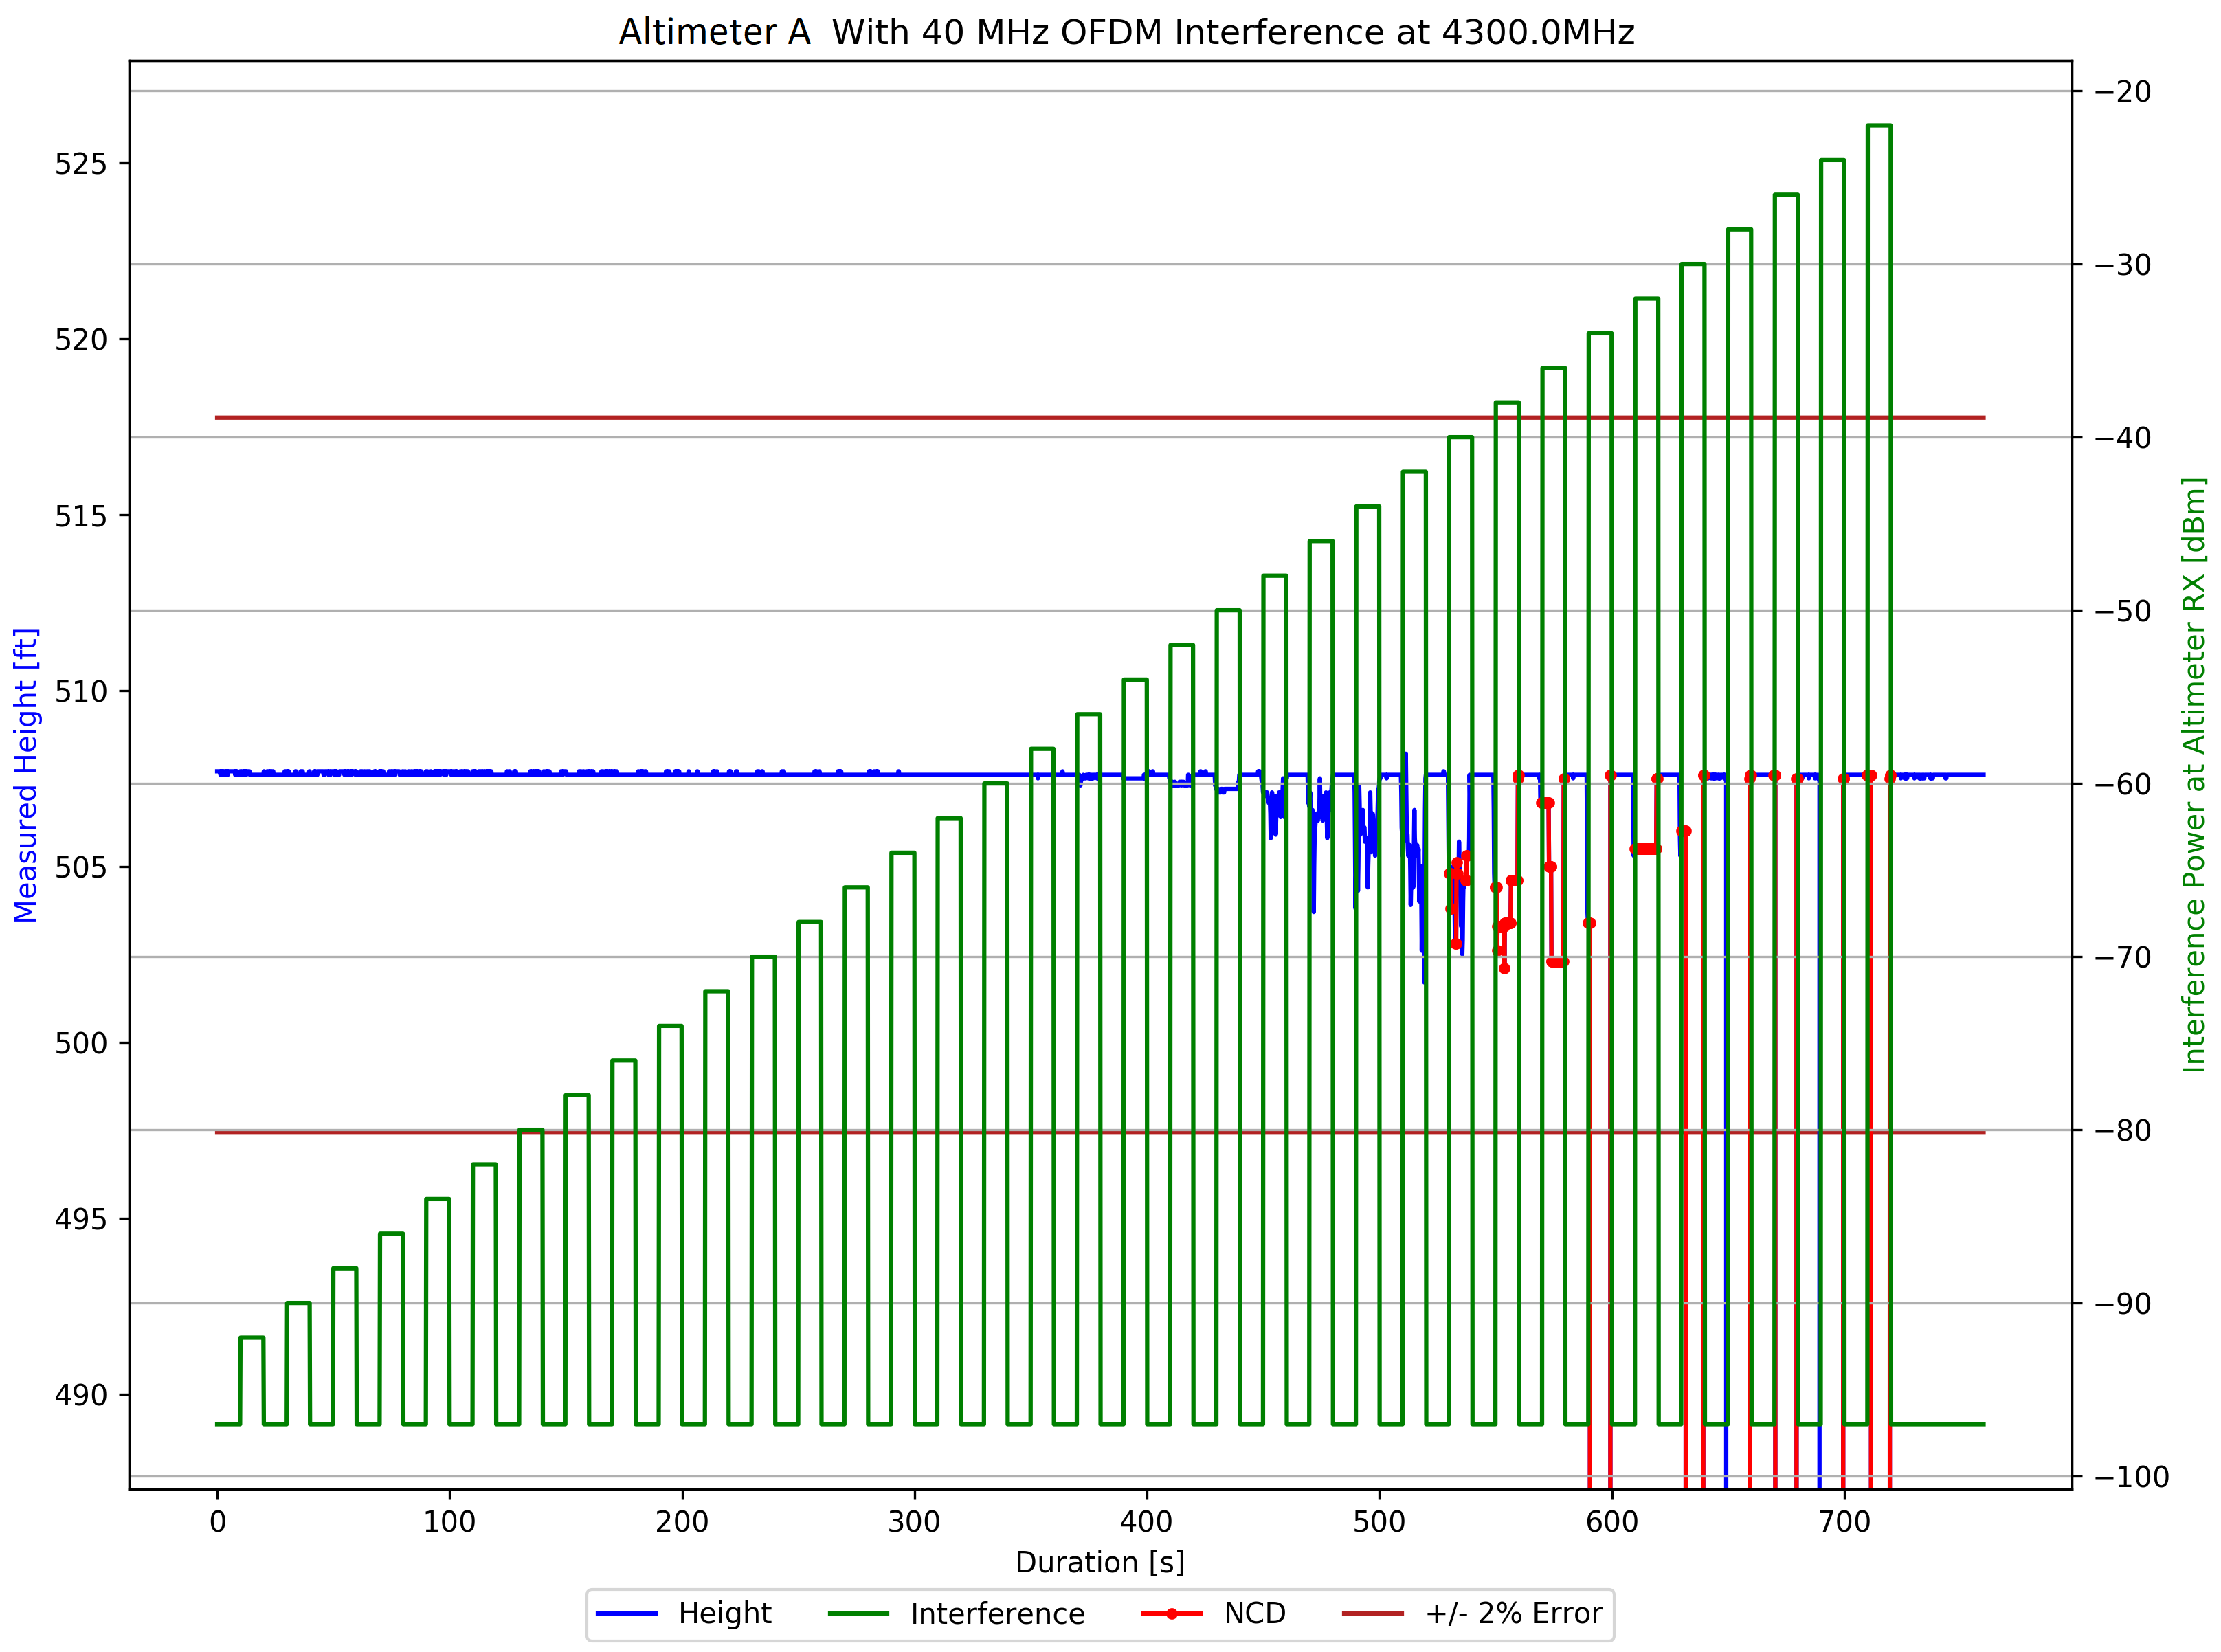
\includegraphics[width=6.0in]{Example_Height_Plot.png}
	\caption{Example Height Plot from Initial Testing Regimen}
	\label{fig:height_plot_example}
\end{figure}
Important information about the test being displayed is contained in the title of each height plot. This includes the altimeter make and model, the bandwidth and modulation format of the interference signal being tested, and the center frequency of RF carrier setting used by the VSG.

The $x$-axis shows the test duration in seconds. After the SQL query sorts by modulation and carrier, the zero second point is set to correspond to the start time for the first RF OFF state for the first interference signal. This time-stamp is subtracted from every mapped data point to yield a plot vs test duration in seconds.

The left hand $y$-axis shows the height output by an altimeter in feet. The axis is centered about \textit{correct height} calculated as the median height before any interference is turned on (See Section~\ref{subsub:nominal}). The upper and lower bounds of this axis correspond to $\pm4$\% error from this correct height respectively. The height signal is plotted with a blue line, but for measurements labeled NCD by the device under test, this is replaced with a bright red marker to clearly show the failure state. Finally, the burgundy lines show the ARINC 707 specified $\pm2$\% error margins. Measurements passing this value constitute a device no longer meeting specifications for certification and are considered severe.  

Finally, the right hand $y$-axis corresponds to the interference power level experienced by the altimeter receiver. The green staircase waveform shows how the RF generator was toggled on and off in increasing power levels over time. To easily signal an OFF state, the OFF state was plotted on the same line as the ON state, with 5~dB subtracted from the minimum interference power used in a test. 

Displaying the data in height plots has numerous advantages. This format clearly shows how an altitude signal is distorted with increasing interference power over time, as well as how quickly the altimeter recovers once the interference is turned off. This format also allows the point in time an altimeter outputs NCD to easily be located. The plots versus time were extremely useful in debugging a test. Errors such as an altimeter which stops outputting data in the middle of a test manifest themselves clearly in a height plot, and manufacturers can correlate this data with recordings of the internal signal processing data stored on SD cards during a test.  

\subsection{Stat Plots}
Despite the advantages stated above, height plots had a disadvantage of being extremely cluttered. When presenting test results to regulators, members of the project management committee tended to spend a disproportionate amount of time discussing the different aspects of the data display as opposed to the results themselves. This motivated the development of stat plots.

Figure~\ref{fig:stat_plot_example} shows an example stat plot made from the same data as the Height Plot in Figure~\ref{fig:height_plot_example}. Stat plots show height error from the correct height versus RF power at the altimeter receiver when the RF power is on. The mean, max, and min are all plotted along with standard deviation error bars and a marker to indicate NCD. Because the noise caused by interference power is not necessarily a normal distribution, the standard deviation error bars do not necessarily have the precise meaning they do with Gaussian noise. However, the error bars do provide a visual representation for how much variance from the mean a given RF power causes. Because of this, they are kept in the plot as a good way to communicate the data.  
\begin{figure}[h!]
	\centering
	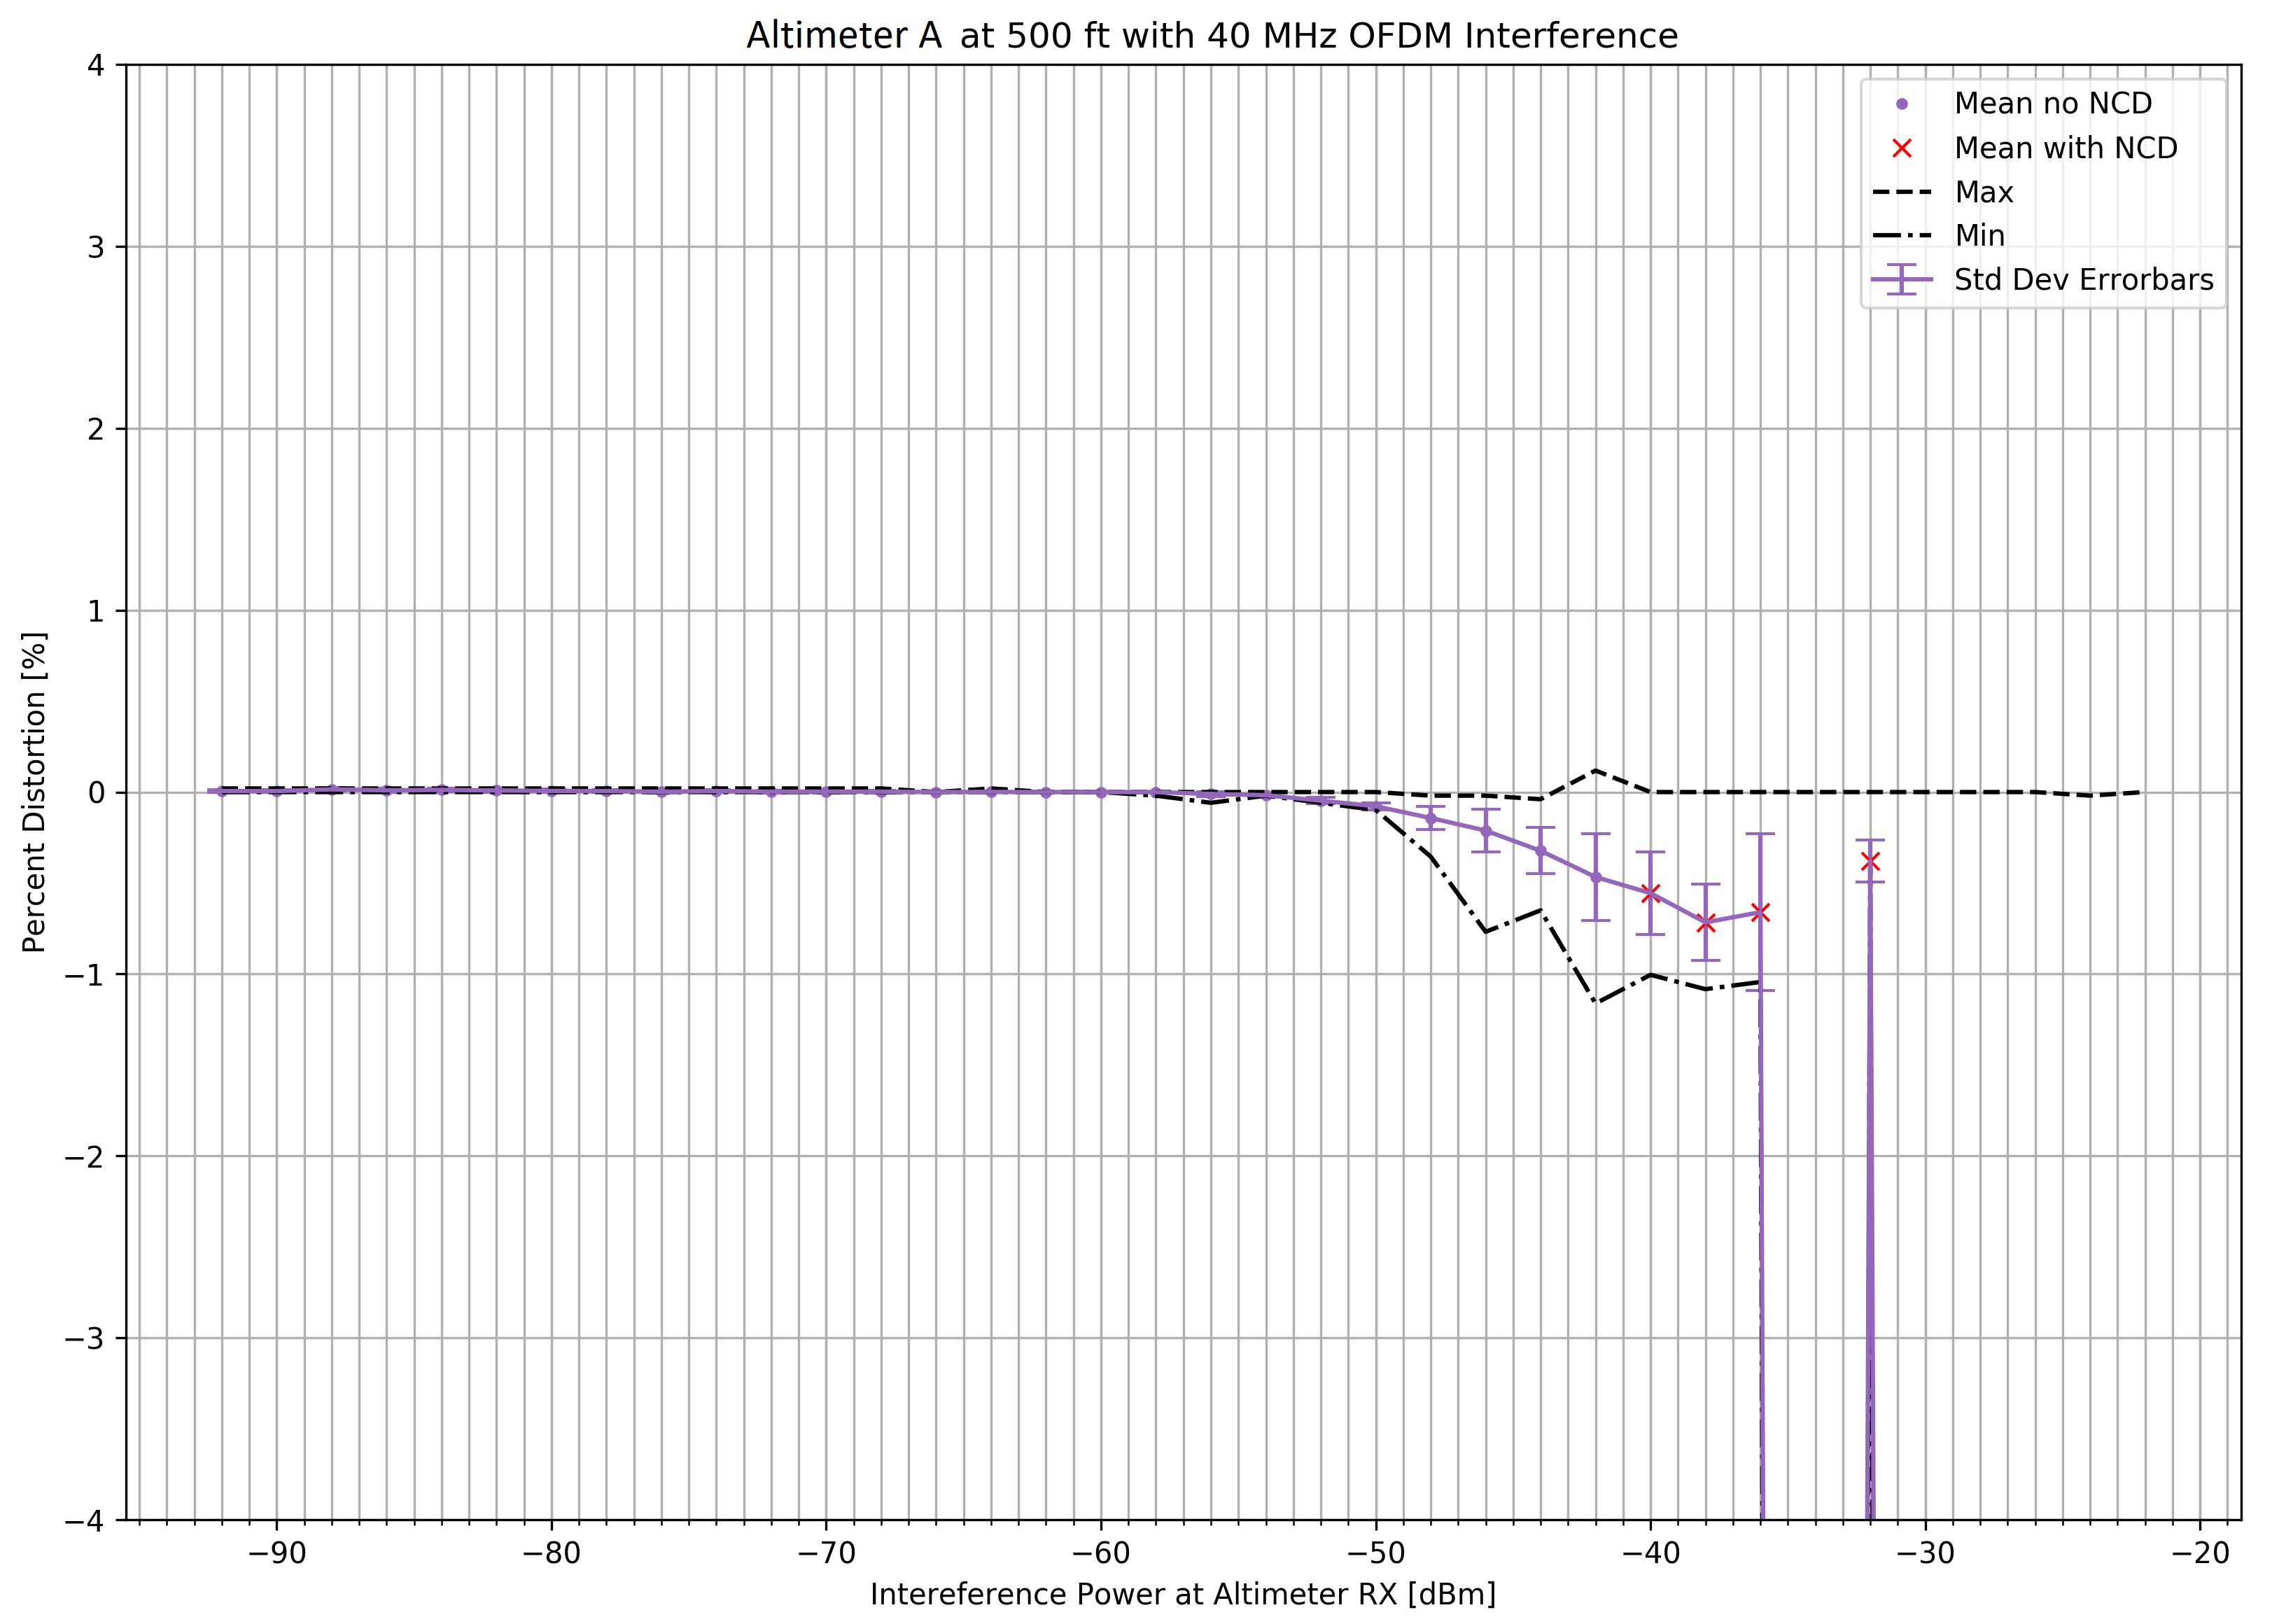
\includegraphics[width=6.0in]{Example_Stat_Plot.png}
	\caption{Example Stat Plot}
	\label{fig:stat_plot_example}
\end{figure}

 Although stat plots do not contain any information about the timing of different events in an altimeter test, they provide a more concise and clean method to display the results of an altimeter test. These features led this representation to be used to communicate test results in letters to the International Civil Aviation Organization (ICAO) Frequency Spectrum Management Panel (FSMP)~\cite{uwe_radio_2019}. 
 
 
\section{Initial `WAIC Only' Testing Regimen}\label{sec:initial_results}

This section covers the results of the initial testing regimen described in Section~\ref{sec:initial}. The `WAIC only' testing was a long term, multifaceted investigation which characterized various aspects of the altimeter response to interference. The test definition from Table~\ref{tab:initial_signals} shows a representative example of a test run with a single altimeter. This would be repeated for the 5 different commercial altimeters sampled for these tests, and for each height the test setup was capable of. 
\begin{figure}[h!]
	\centering
	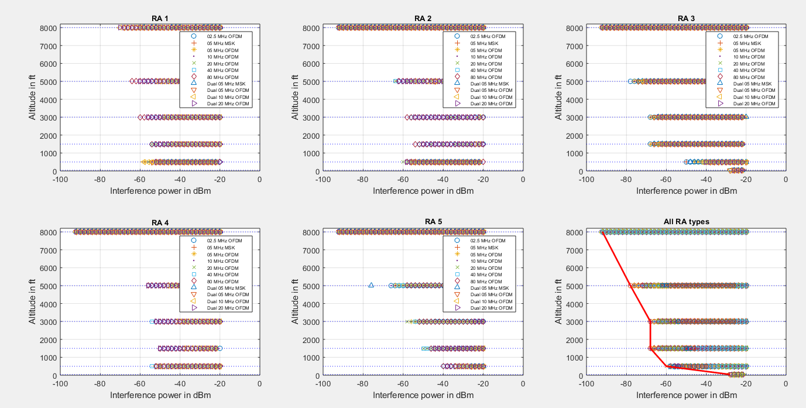
\includegraphics[width=6.0in]{Initial_Summary.png}
	\caption{Summary of Initial Testing Results Presented to the FSMP in~\cite{uwe_radio_2019}}
	\label{fig:initial_summary}
\end{figure}

Figure~\ref{fig:initial_summary} shows a comprehensive summary of these results. Each data point on shows the results of a single altimeter test equivalent to a height plot in Figure~\ref{fig:height_plot_example}. The data points plot the power level at which the altimeter under test goes beyond a mean error of $\pm0.5\%$. This plot served as an introduction to the presentation of the results of the second and third testing regimens~\cite{uwe_radio_2019}, as a means of showing how the WAIC only tests justified further investigation. 

Early tests investigated the proper loop loss value to use. Although loop losses were specified in DO-155 (see Section~\ref{subsub:loss}), it was ambiguous as to whether the loop losses were to be measured between the ports of the altimeter or between the ports of the altitude simulator. While the language in the regulations made it seem intuitive to place the loop loss between the ports of the altitude simulator, the additional cable loss leading to and from the simulator made the altimeters unable to function. It was hypothesized that the worst case scattering coefficients in use for the loop loss calculation made the addition of cabling turn an already conservative case to an unrealistic one. Because these units were all certified, the loop loss was moved to the ports of the altitude simulator to ensure functionality, and this was noted in any communication of results to outside parties.

A series of tests during the initial testing regimen placed a 10~MHz OFDM signal at different points in the altimeter band. These showed that the altimeter under test consistently broke at lower power levels when interference was injected at the center of the band than at the outer edges. Subsequent testing only centered simulated WAIC waveforms at the center of the band to provide the most conservative results. 
\begin{figure}[h!]
	\centering
	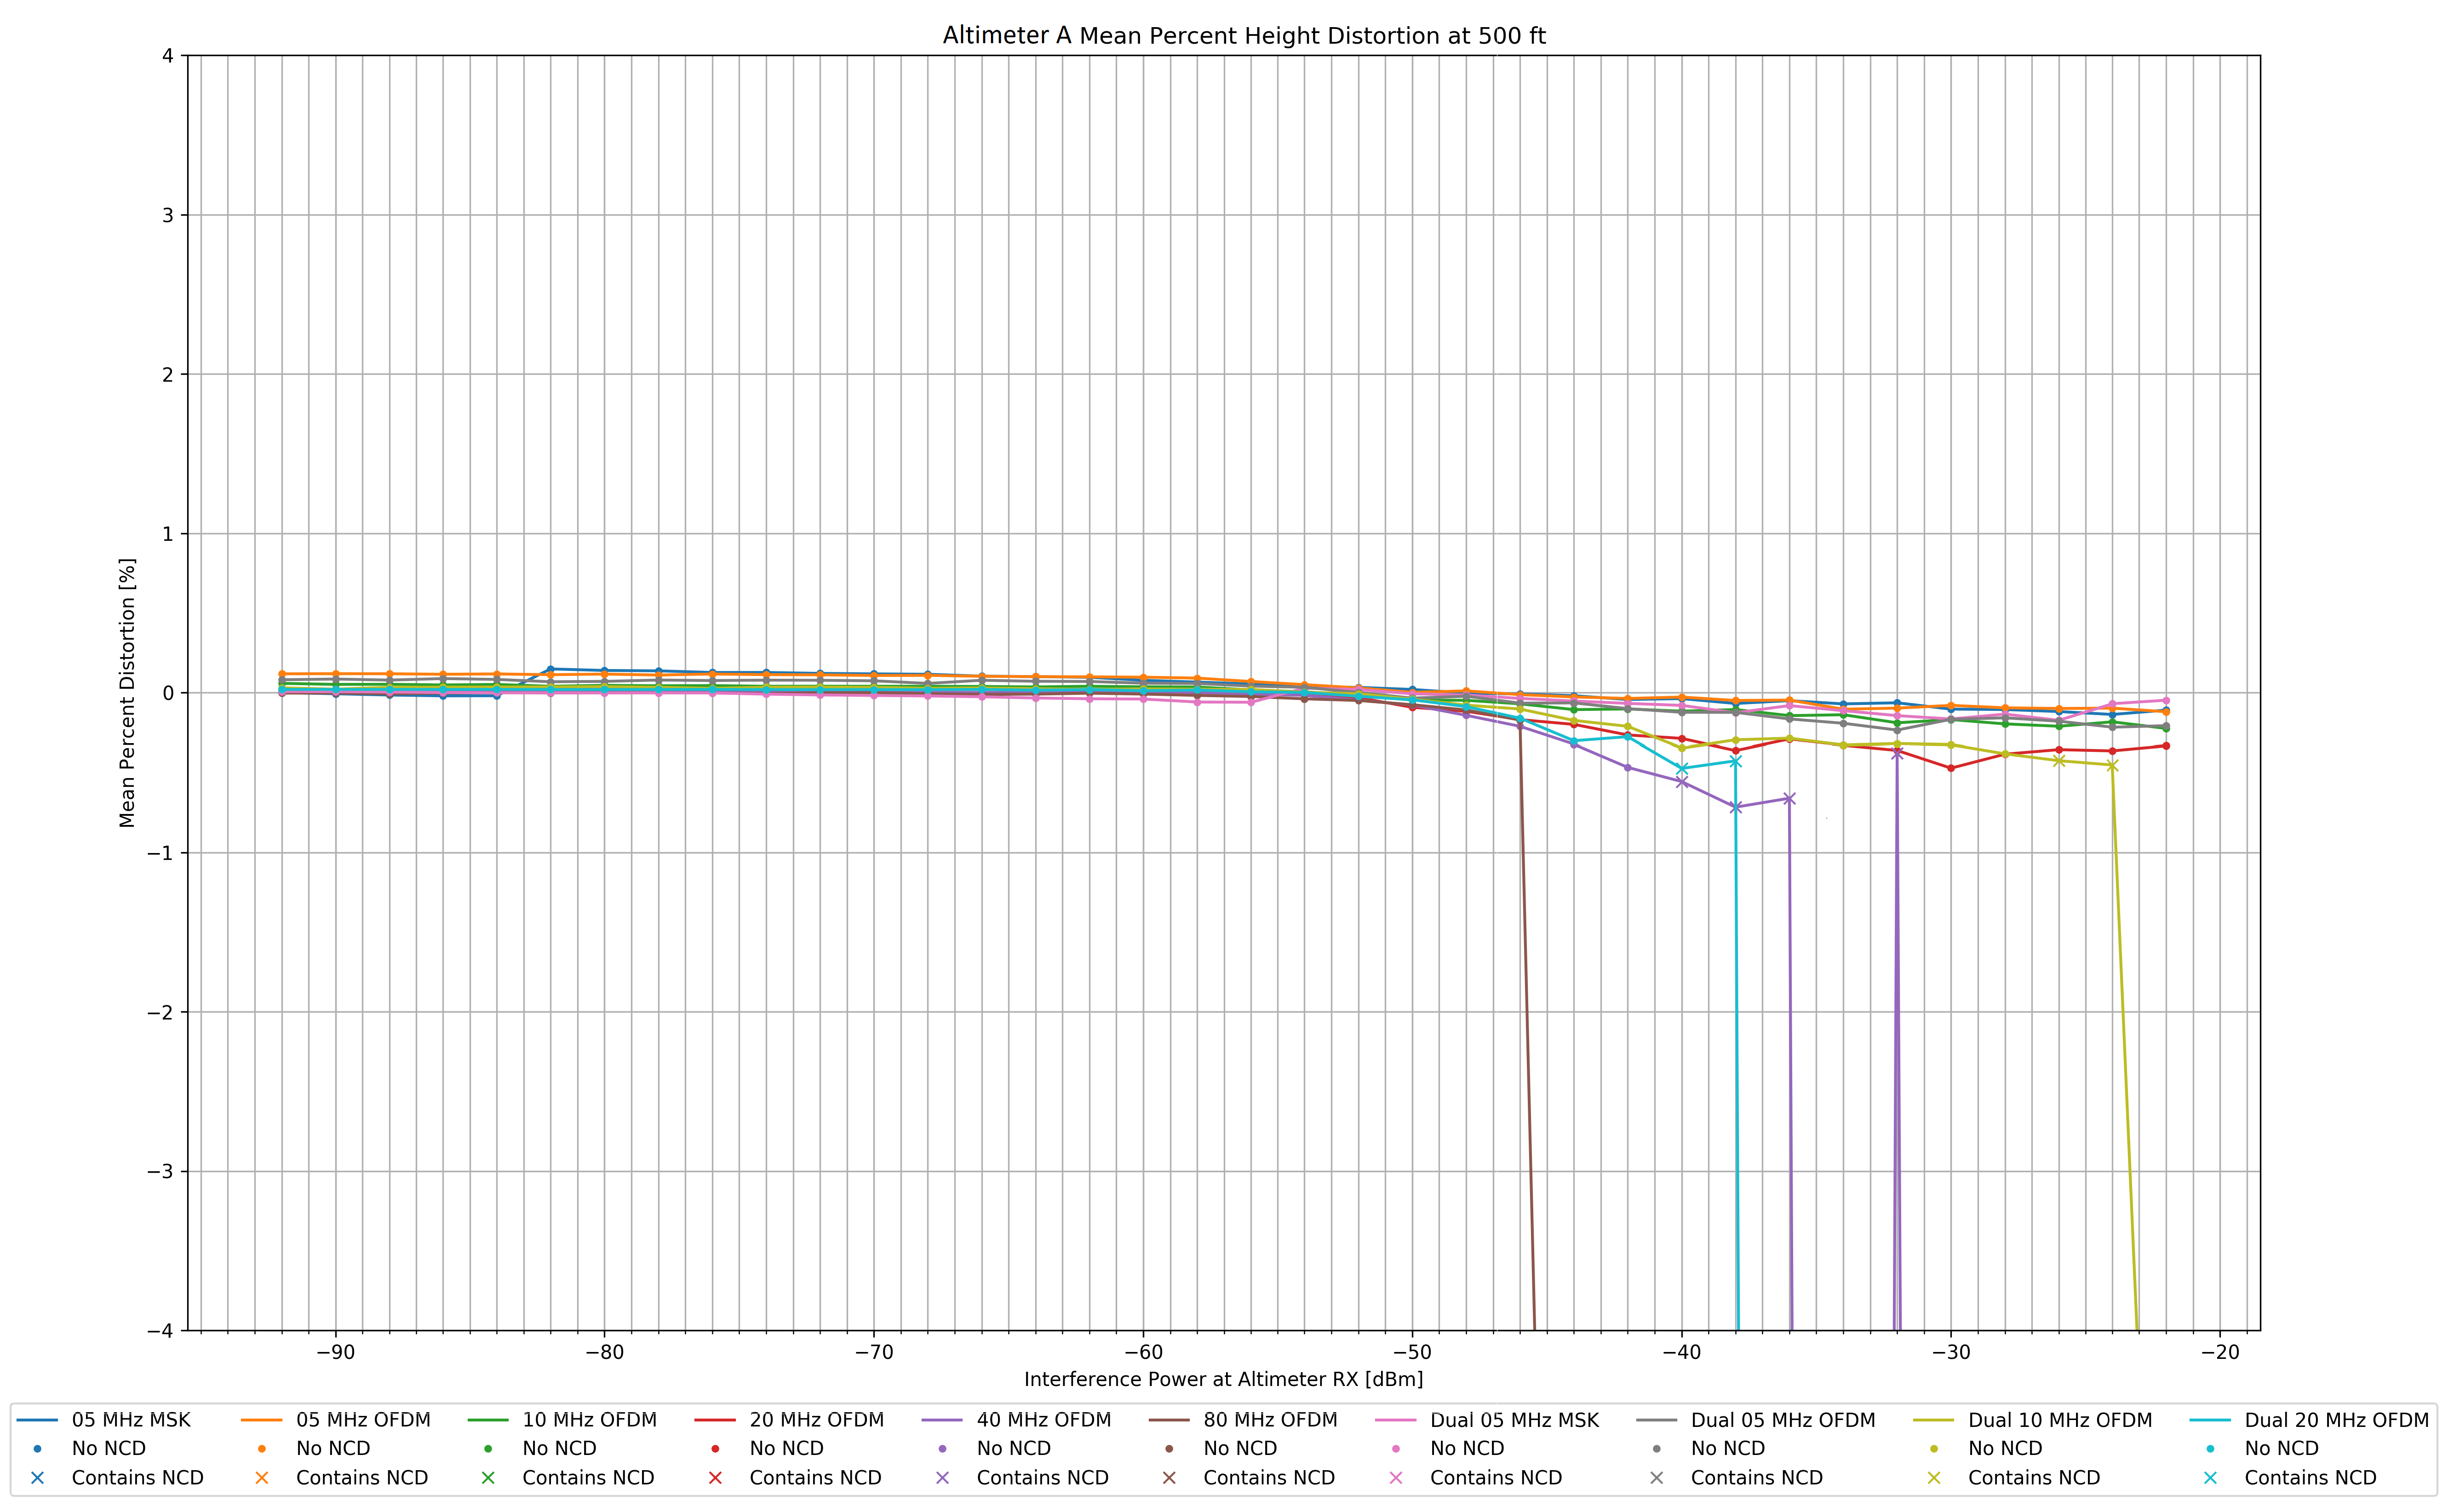
\includegraphics[width=6.0in]{Mean_Comparison_Example.png}
	\caption{Comparison of Impact of Different Bandwidths of Simulated WAIC Signals on Altimeter Performance}
	\label{fig:mean_comparison}
\end{figure}
Finally, these tests investigated the effects of interference bandwidth on altimeter performance, and the effects of separating a waveform into a `dual' version of the waveform with a $\pm20$~MHz offset from the center. The test definition shown in Table~\ref{tab:initial_signals} was the last iteration of the test procedure run before expanding the setup, and functions to demonstrate these effects. Figure~\ref{fig:mean_comparison} shows a stat plot comparing the mean height error caused by interference signals of increasing bandwidth. These results consistently showed that wider bandwidth interference caused worse altimeter performance. Although dual waveforms helped performance, their impact was inconsistent.  

These results were used to justify expanding the test setup and measuring altimeter response to wider bandwidth WAIC signals aggregated with interference from other altimeters to provide a realistic worst case scenario.

\section{Expanded In Band Tests}\label{sec:dvsg_ib_results}
This section discusses the results of the testing regimen described in Section~\ref{sub:ib}. The goal of this iteration of tests was to measure the response of altimeters to a full band of simulated WAIC interference, in the presence of simulated interference from other altimeters. The combined interference represented a more conservative than the real life worse case scenario for altimeter interference. Five different altimeters were tested: the Rockwell Collins LRA2100, The Rockwell Collins LRA900, the Thales ERT530, the Thales ERT550, and the Honeywell ALA52B.
 \begin{figure}[h!]
	\centering
	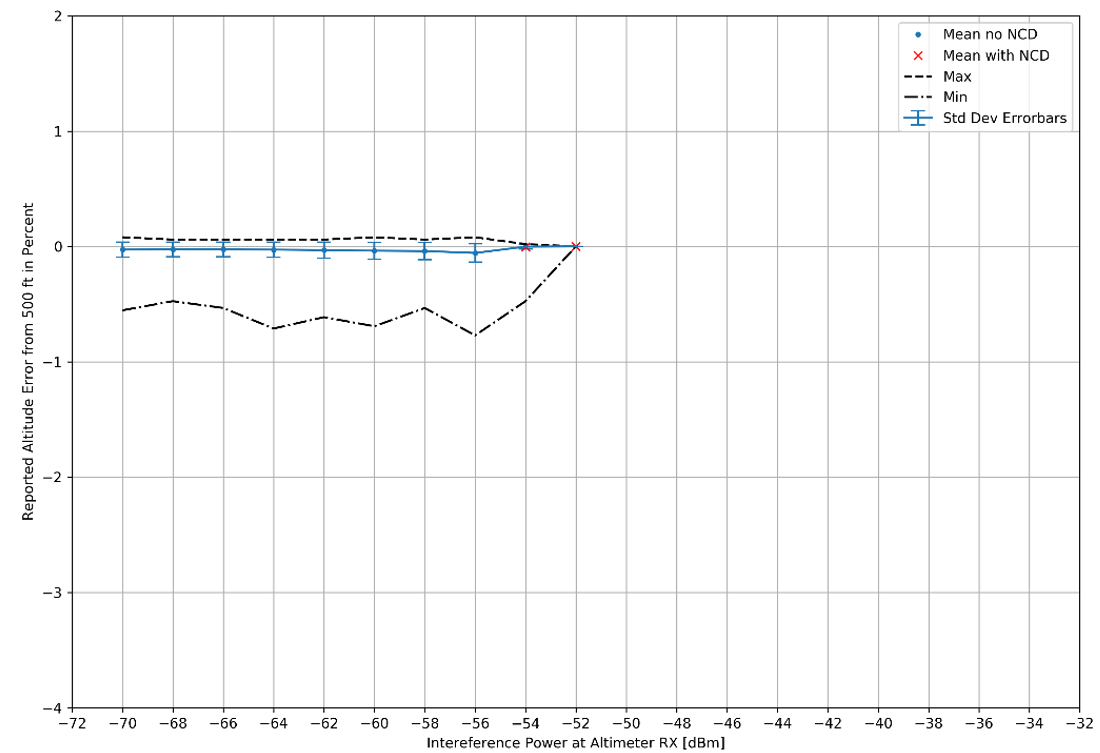
\includegraphics[width=6.0in]{RA4_ib_results.png}
	\caption{Performance of RA Type 4 with 200MHz In Band Tests}
	\label{fig:RA4}
\end{figure}

 % Please add the following required packages to your document preamble:
% \usepackage{booktabs}
\begin{table}[]
\begin{tabular}{@{}cccccc@{}}
\toprule
                            & RA Type 1 & RA Type 2 & RA Type 3 & RA Type 4 & RA Type 5 \\ \midrule
WAIC Interference Threshold & -54 dBm   & -56 dBm   & -44 dBm   & -56 dBm*  & -44 dBm   \\ \bottomrule
\end{tabular}
\caption{Interference power level above which reported altitude is impacted~\cite{uwe_radio_2019}}
\label{tab:ib_thresholds_fsmp}
\end{table}

The breaking point of each was found according to Section~\ref{sub:break}, and these were used to propose maximum radiated power thresholds to the FSMP~\cite{uwe_radio_2019}. The resulting minimum power thresholds, with altimeter names redacted, are shown in Table~\ref{tab:ib_thresholds_fsmp}. RA Type~4 performed the worst of the five models tested, so the final threshold recommended to the FSMP was 56 dBm based on this failure point. Figure~\ref{fig:RA4} 
 shows the results of this altimeter. The first breaking point occurs at -54~dBm interference power at the altimeter receiver, thus the WAIC threshold was set at -56~dBm. The results of the remaining altimeters are shown in Appendix~\ref{appendix_a} for completeness. 

\section{Out of Band Testing}\label{sec:dvsg_oob_results}
 \begin{figure}[h!]
	\centering
	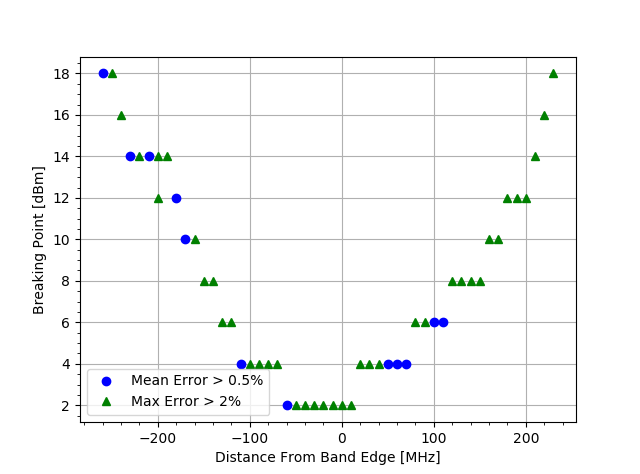
\includegraphics[width=3.5in]{oob_mask.png}
	\caption{Preliminary Interference Mask}
	\label{fig:oob_mask}
\end{figure}

This section covers the results of the out of band testing regimen described in Section~\ref{sub:oob}. This test used the same expanded test setup as the 200~MHz in-band tests. VCOs were used to simulate external altimeter signals at a 200~ft approach, and one of the VSG's generated 130~MHz wide simulated WAIC interference. The second VSG stepped RF signals out from the band edges. The goal was to find how the breaking point changed with distance from the band edge in MHz. An example of these results plotted is shown in Figure~\ref{fig:oob_mask}. These tests are still in progress at the time of writing, but like the results in Section~\ref{sec:dvsg_ib_results}, are expected to justify reccomendations made to regulators for safe power thresholds in the adjacent bands. 


%%%%%%%%%%%%%%%%%%%%%%%%%%%%%%%%%%%%%%%%%%%%%%%%%%%
%
%  New template code for TAMU Theses and Dissertations starting Fall 2016.  
%
%
%  Author: Sean Zachary Roberson
%  Version 3.17.09
%  Last Updated: 9/21/2017
%
%%%%%%%%%%%%%%%%%%%%%%%%%%%%%%%%%%%%%%%%%%%%%%%%%%%
%%%%%%%%%%%%%%%%%%%%%%%%%%%%%%%%%%%%%%%%%%%%%%%%%%%%%%%%%%%%%%%%%%%%%%
%%                           SECTION IV
%%%%%%%%%%%%%%%%%%%%%%%%%%%%%%%%%%%%%%%%%%%%%%%%%%%%%%%%%%%%%%%%%%%%%



\chapter{CONCLUSION \label{cha:Summary}}

This work covered the development of a reference test bed for radio altimeter interference suceptibility testing which was validated by altimeter manufacturers and aircraft manufacturers. The test bed was automated in a modular framework which allowed rapid modification to enable testing under a wide range of conditions. Finally, this work covers the support the author gave to the execution, and analysis of data from radio altimeter tests. The reporting formats created supported the development of international standards for wireless avionics. These include: the International Civil Aviation Organization Standard and Reccommended Practices (ICAO SARPs), RTCA inc. Minimum Aviation System Performance Standards (RTCA MASPS), and Minimum Operational Performance Standards (RTCA MOPS).  In the future, the wireless avionics equipment governed by these standards will allow air travel to become safer, more fuel efficient, and more economical. 
%The next line is the format for inserting new sections.
%Replace the name "newsection"  with the name of your
%new section file.
%\include{data/newsection}

%fix spacing in bibliography, if any...
%%%%%%%%%%%%%%%%%%%%%%%%%%%%%%%%%%%%%%%%%%%%%%%%%%%%%%%%%%%%%
\let\oldbibitem\bibitem
\renewcommand{\bibitem}{\setlength{\itemsep}{0pt}\oldbibitem}
%%%%%%%%%%%%%%%%%%%%%%%%%%%%%%%%%%%%%%%%%%%%%%%%%%%%%%%%%%%%%%%
%The bibliography style declared is the IEEE format. If
%you require a different style, see the document
%bibstyles.pdf included in this package. This file,
%hosted by the University of Vienna, shows several
%bibliography styles and examples of in-text citation
%and a references page.
\bibliographystyle{ieeetr}

\phantomsection
\addcontentsline{toc}{chapter}{REFERENCES}

\renewcommand{\bibname}{{\normalsize\rm REFERENCES}}

%This file is a .bib database that contains the sources.
%This removes the dependency on the previous file
%bibliography.tex.
\bibliography{data/Masters_Thesis}




%This next line includes appendices. The file
%appendix.tex contains commands pointing to
%the appendix files; be sure to change these
%pointers if you end up changing the filenames.
%Leave this commented if you will not need
%appendix material.
%%%%%%%%%%%%%%%%%%%%%%%%%%%%%%%%%%%%%%%%%%%%%%%%%%%
%
%  New template code for TAMU Theses and Dissertations starting Fall 2016.  
%
%
%  Author: Sean Zachary Roberson
%  Version 3.17.09
%  Last Updated: 9/21/2017
%
%%%%%%%%%%%%%%%%%%%%%%%%%%%%%%%%%%%%%%%%%%%%%%%%%%%

\begin{appendices}
\titleformat{\chapter}{\centering\normalsize}{APPENDIX \thechapter}{0em}{\vskip .5\baselineskip\centering}
\renewcommand{\appendixname}{APPENDIX}

%%%%%%%%%%%%%%%%%%%%%%%%%%%%%%%%%%%%%%%%%%%%%%%%%%%
%
%  New template code for TAMU Theses and Dissertations starting Fall 2016.
%
%
%  Author: Sean Zachary Roberson 
%	 Version 3.16.09
%  Last updated 9/12/2016
%
%%%%%%%%%%%%%%%%%%%%%%%%%%%%%%%%%%%%%%%%%%%%%%%%%%%

%%%%%%%%%%%%%%%%%%%%%%%%%%%%%%%%%%%%%%%%%%%%%%%%%%%%%%%%%%%%%%%%%%%%%%
%%                           APPENDIX A 
%%%%%%%%%%%%%%%%%%%%%%%%%%%%%%%%%%%%%%%%%%%%%%%%%%%%%%%%%%%%%%%%%%%%%

\phantomsection

\chapter{\uppercase{Full Results for In Band Testing}}\label{appendix_a}

The results of all five altimeters presented to the FSMP in~\cite{schwark_radio_2019} are presented here. The results were summarized in Table~\ref{tab:ib_thresholds_fsmp}. The breaking point was as described in Section~\ref{sub:break}, and consists of any reported altitude (i) labeled NCD (ii) with a maximum height error $\geq\pm2\%$, or (iii) any mean height error $\geq\pm5\%$. Interference power thresholds were then set 2~dB below the breaking point of the worst performing altimeter (RA Type 4). 
 \begin{figure}[h!]
	\centering
	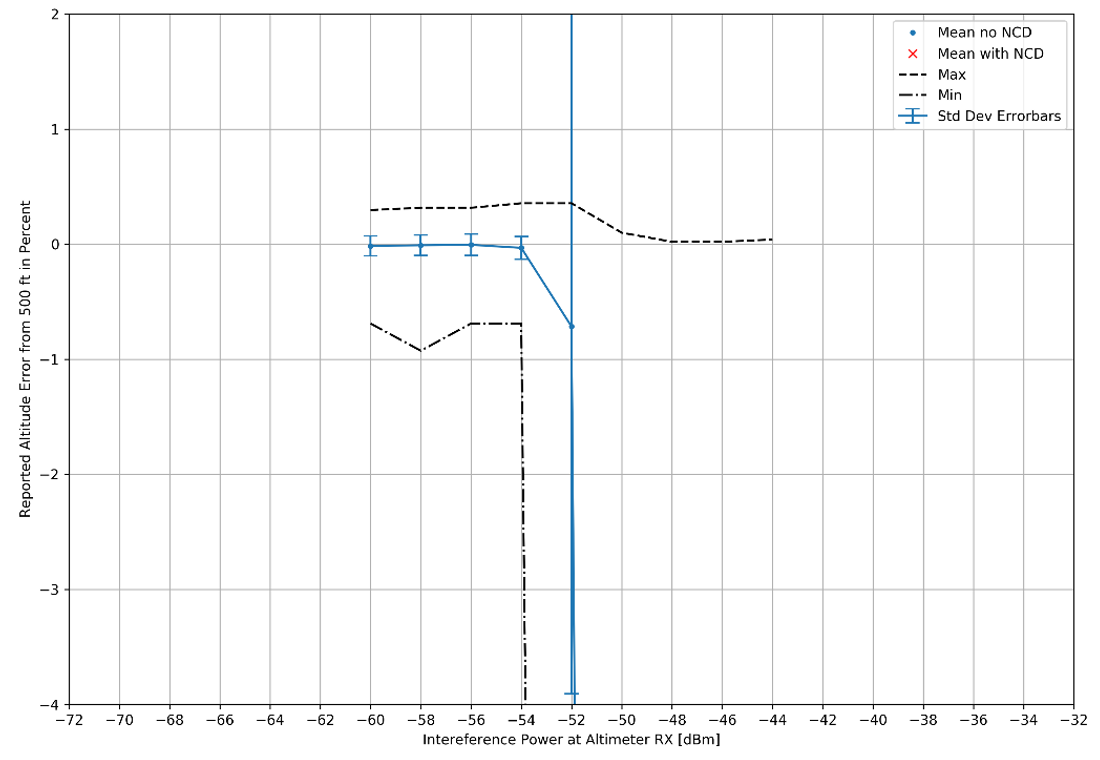
\includegraphics[width=5.0in]{RA1_ib_results.png}
	\caption{Performance of RA Type 1 with 200MHz In Band Tests}
	\label{fig:RA1}
\end{figure}

 \begin{figure}[h!]
	\centering
	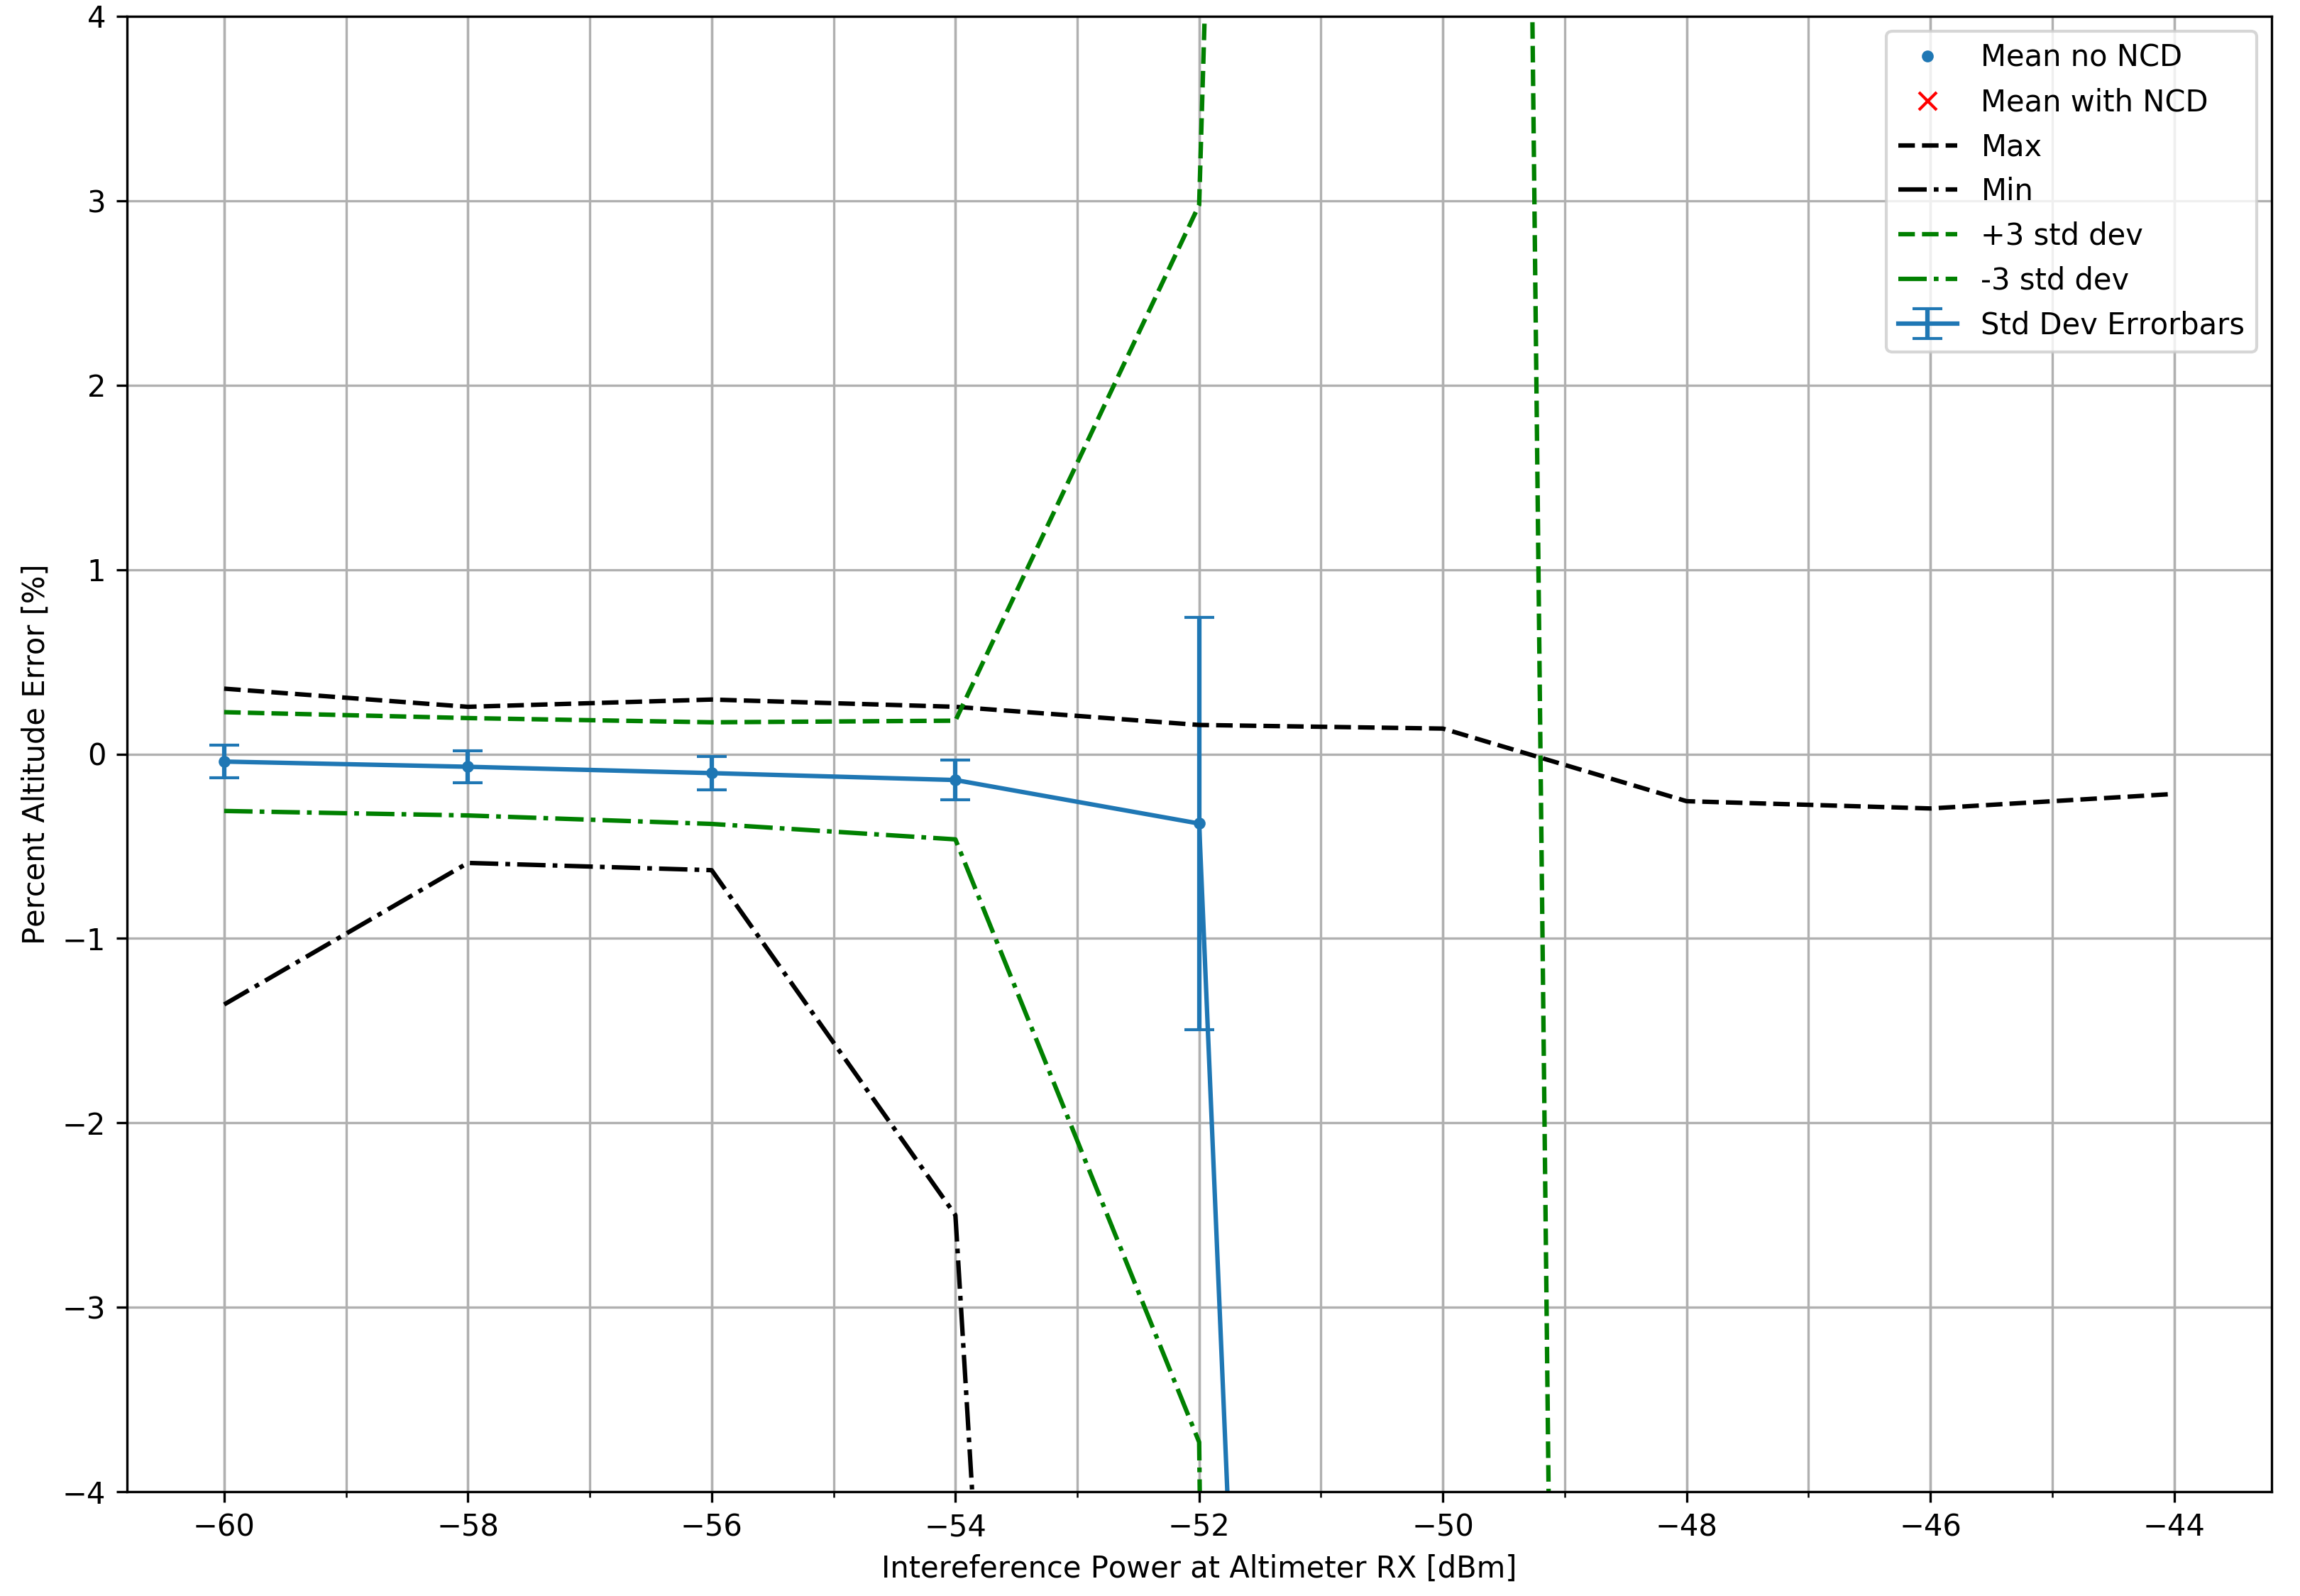
\includegraphics[width=5.0in]{RA2_ib_results.png}
	\caption{Performance of RA Type 2 with 200MHz In Band Tests}
	\label{fig:RA2}
\end{figure}

 \begin{figure}[h!]
	\centering
	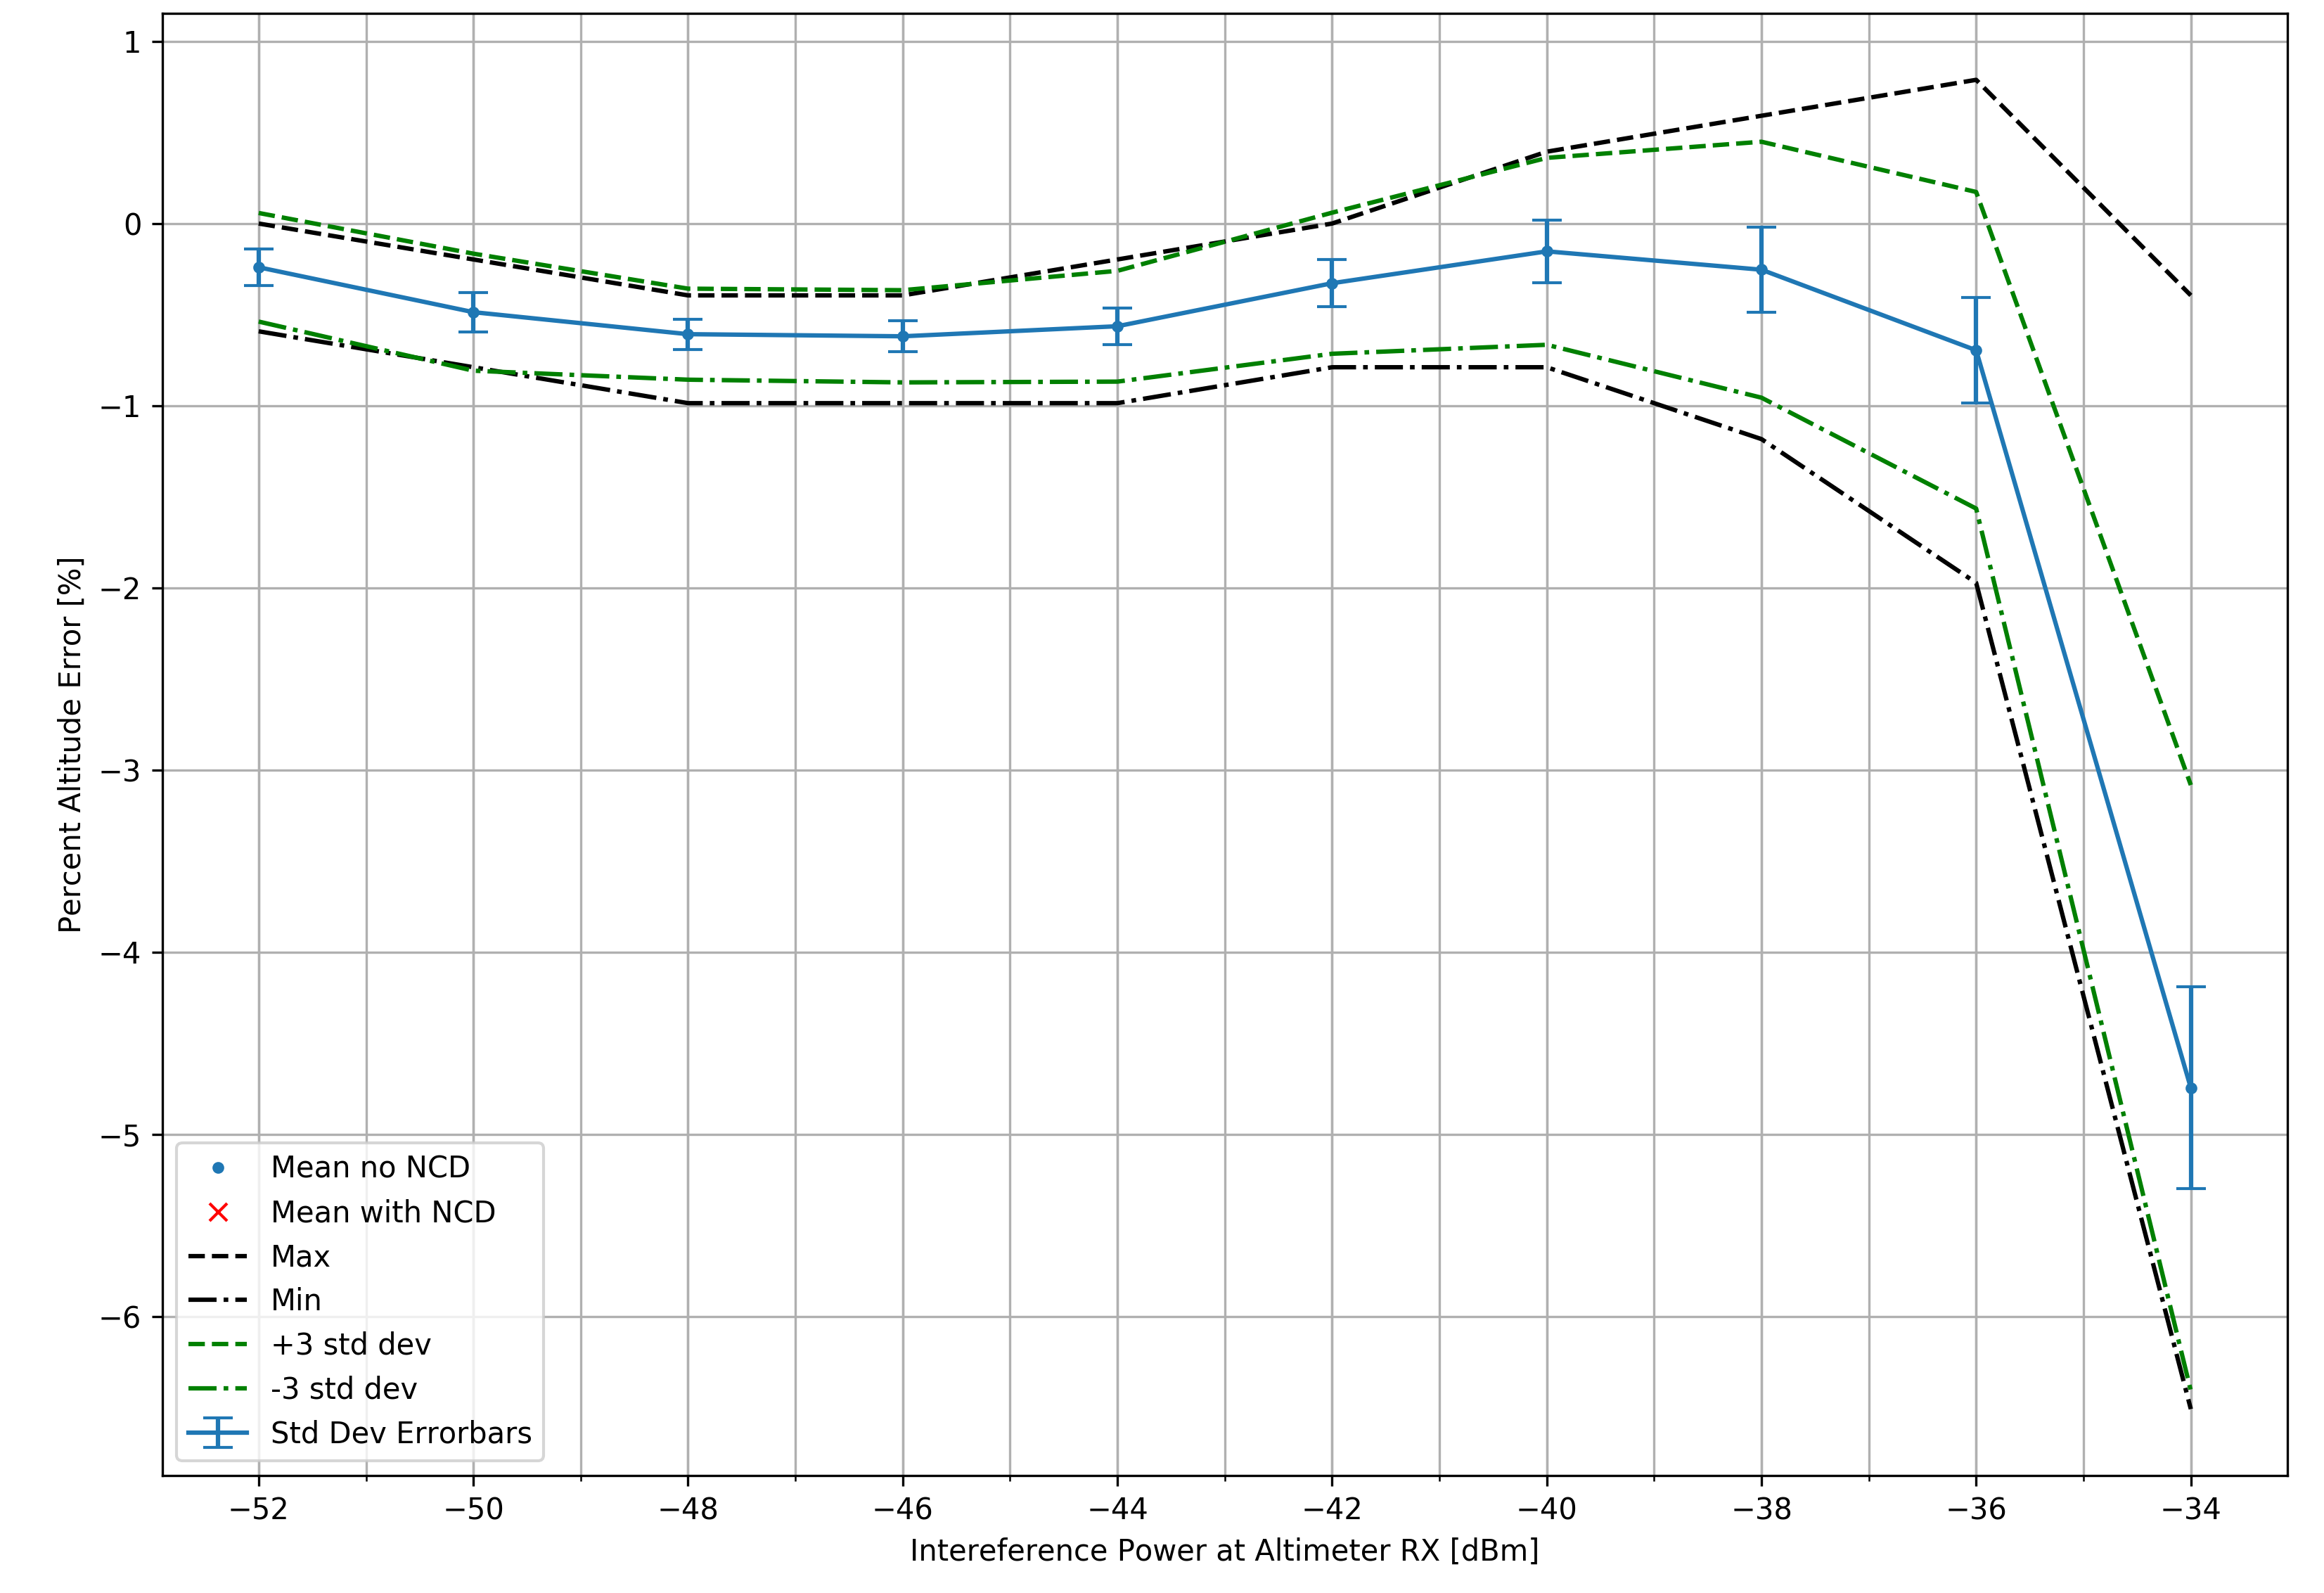
\includegraphics[width=5.0in]{RA3_ib_results.png}
	\caption{Performance of RA Type 3 with 200MHz In Band Tests}
	\label{fig:RA3}
\end{figure}

 \begin{figure}[h!]
	\centering
	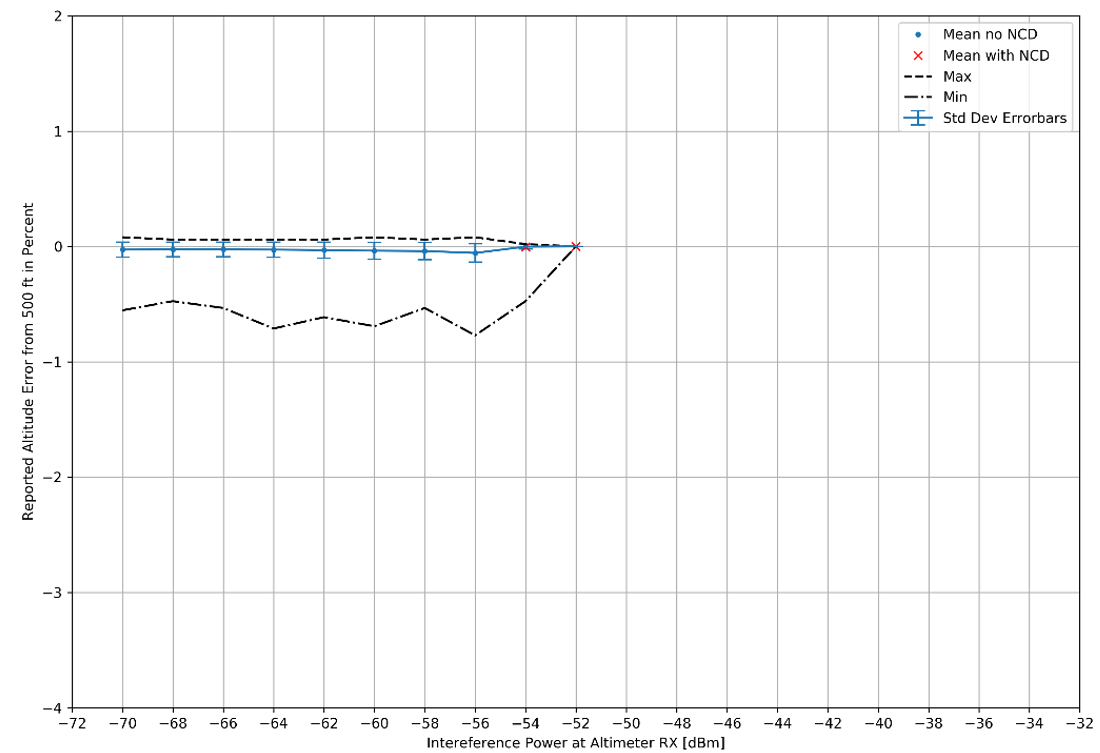
\includegraphics[width=5.0in]{RA4_ib_results.png}
	\caption{Performance of RA Type 4 with 200MHz In Band Tests}
	\label{fig:RA4_appendix}
\end{figure}

 \begin{figure}[h!]
	\centering
	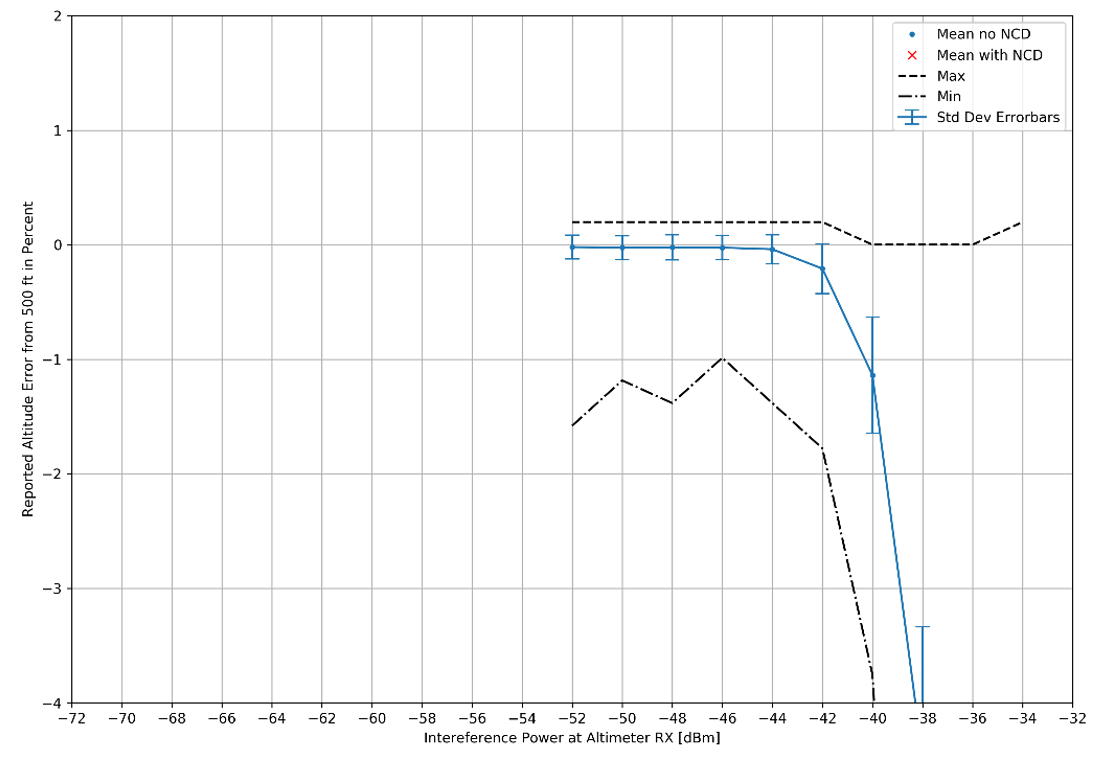
\includegraphics[width=5.0in]{RA5_ib_results.png}
	\caption{Performance of RA Type 5 with 200MHz In Band Tests}
	\label{fig:RA5}
\end{figure}

%%%%%%%%%%%%%%%%%%%%%%%%%%%%%%%%%%%%%%%%%%%%%%%%%%%%
%
%  New template code for TAMU Theses and Dissertations starting Fall 2016.
%
%
%  Author: Sean Zachary Roberson 
%	 Version 3.16.09 
%  Last updated 9/12/2016
%
%%%%%%%%%%%%%%%%%%%%%%%%%%%%%%%%%%%%%%%%%%%%%%%%%%%

%%%%%%%%%%%%%%%%%%%%%%%%%%%%%%%%%%%%%%%%%%%%%%%%%%%%%%%%%%%%%%%%%%%%%%
%%                           APPENDIX B
%%%%%%%%%%%%%%%%%%%%%%%%%%%%%%%%%%%%%%%%%%%%%%%%%%%%%%%%%%%%%%%%%%%%%

\chapter{\uppercase {A Second Appendix Whose Title Is Much Longer Than The First}}

Text for the Appendix follows.

\begin{figure}[h]
\centering
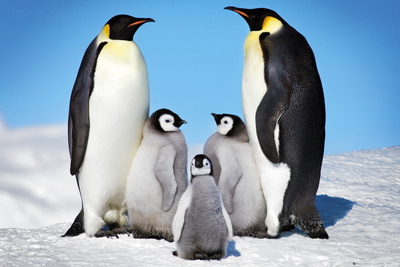
\includegraphics[scale=.50]{figures/Penguins.jpg}
\caption{Another TAMU figure.}
\label{fig:tamu-fig6}
\end{figure}

\section{Appendix Section}

\section{Second Appendix Section}


\pagebreak{}

\end{appendices}


\end{document}
